\documentclass{article}
\usepackage{graphicx}
\usepackage[section]{placeins}
\makeatletter
\AtBeginDocument{%
  \expandafter\renewcommand\expandafter\subsection\expandafter{%
    \expandafter\@fb@secFB\subsection
  }%
}
\makeatother

\usepackage{geometry}
 \geometry{
 a4paper,
 left=15mm,
 right=15mm,
 top=15mm,
 bottom=20mm,
 }

\title{DUNE Flux Predicition Uncertainties for the DUNE Far Detector Technical Design Review Analysis}
\author{Luke Pickering}
\date{\today}

\begin{document}
\maketitle

\abstract{This Technical note describes an update of the DUNE flux  prediction prior uncertainties. It is meant to be read in the context of previous notes \cite{} and \cite{}. The two significant additions in this analysis are the inclusion of a range of near detector predictions off axis for use in DUNE-PRISM studies and the description of ready-to-use flux uncertainty tools based on an eigenvalue decomposition of the total flux matrix.}

\section{TODO}

\begin{itemize}
\item TODO: Add description of supplied tools
\end{itemize}

\section{Flux Predictions}

All beamline simulations in this document were produced using \texttt{g4lbne v3r5p4}, \texttt{GEANT 4.10.3p3}, and where applicable a slightly modified version of \texttt{PPFX vX}\footnote{No physics modifications were made so these results should be exactly reproducible}. The predictions were based upon the macro \texttt{OptimizedEngineeredNov17.mac}, which was modified where neccessary to move beamline components or alter running conditions. Hadron and muon decays that produce neutrinos are the output of the beamline simulation, these decays were sampled to produce neutrino flux predictions through predefined volumes by use of the \texttt{dk2nu v01.05.01} package.

\subsection{Flux Volumes}

Each decaying hadron is simulated to decay such that the final state neutrino is forced to go through a relevant flux volume, the neutrino ray end position within the volume is randomly sampled. Volumes are used rather than the more-common two dimensional planes to avoid subleties in solid-angle coverage for a detector that moves off axis and has a significant extent in the beam direction (\emph{i.e.} A flux plane on the front face of a detector which has extent in the normal to the plane, would result in a different prediction than a similar flux plane on the back face of the detector if that detector volume was significantly off beam axis. Averaging over the whole volume get around this). The assumed volume is 4x2x3 (WxHxL) which corresponds to expected fiducial volume of the DUNE-PRISM oscillation analysis. It is possible that the on-axis only analysis would use a wider fiducial volume in $\hat{x}$, but predictions will be shown for a contiguous line of such volumes across the expected off axis range, 0--32.5~m. The near detector is placed 562~m downstream of the \texttt{g4lbnf} geometry origin (\texttt{MCZER0}), in accordance with the engineering drawing shown in \ref{fig:flux_predictions__NDHallDef}. The precise z positioning of the far detector is less important, and is taken to be 1300~km downstream of the \texttt{g4lbnf} geomtry origin, here a simple flux plane is used as there is no significant variation over the $\mathcal{O}(10)$ m extent of the far detector volume.

\begin{figure}
  \centering
  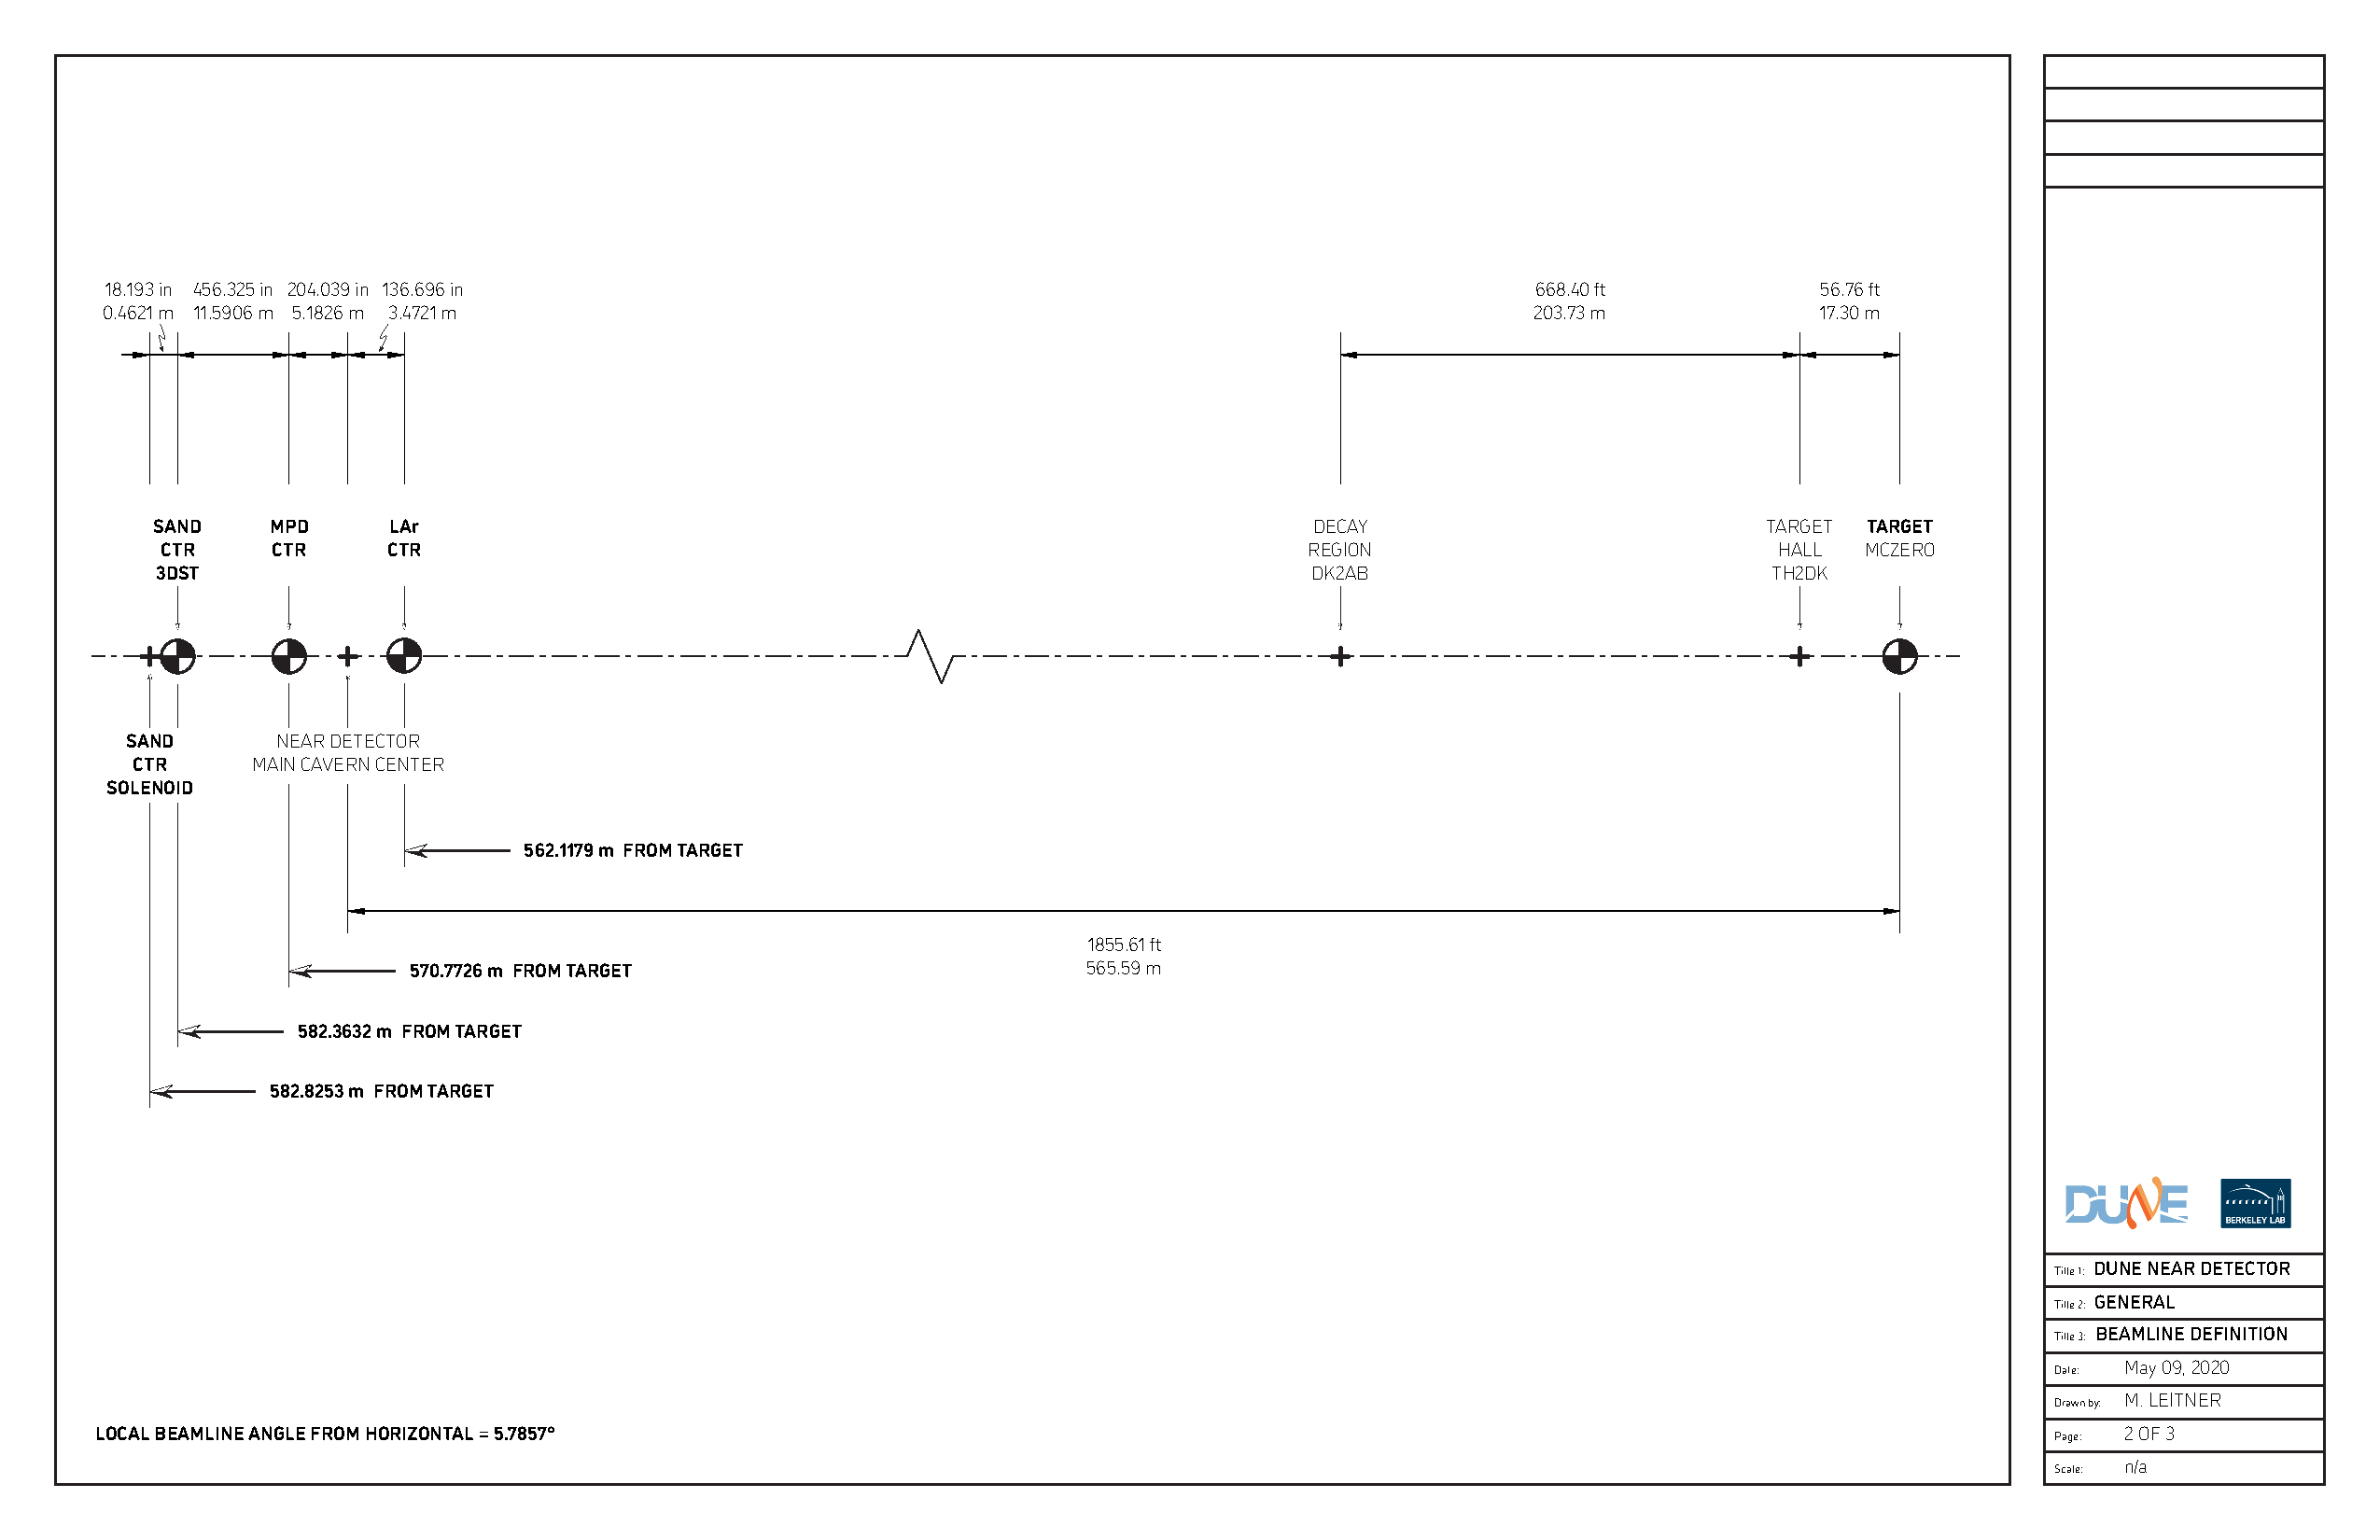
\includegraphics[width=0.95\textwidth]{plots/BEAMLINEDEFINITION}
  \caption{The relative positions of beamline geometry and the center of the liquid argon detector.}
  \label{fig:flux_predictions__NDHallDef}
\end{figure}

\subsection{Nominal Predictions}

The 'nominal' near detector (574 m) flux prediction for each horn polarity, neutrino species, and for 6 on- and off-axis positions can be see in Fig.\ref{fig:flux_predictions__on_axis}--\ref{fig:flux_predictions__off_axis}. In addition to making off axis near detector measurements, it has been shown that making measurements at a lower horn current can significantly enhance the DUNE-PRISM program, the relative flux predictions when running the horns at 280~kA, instead of the nominal 293~kA, can be seen in \ref{fig:flux_predictions__on_axis_lower_HC}. The detailed motivation of 280~kA special runs will not be discussed in this document, but the effect of hadron production uncertainties on the 293~kA and the 280~kA will be compared.

\begin{figure}
  \centering
  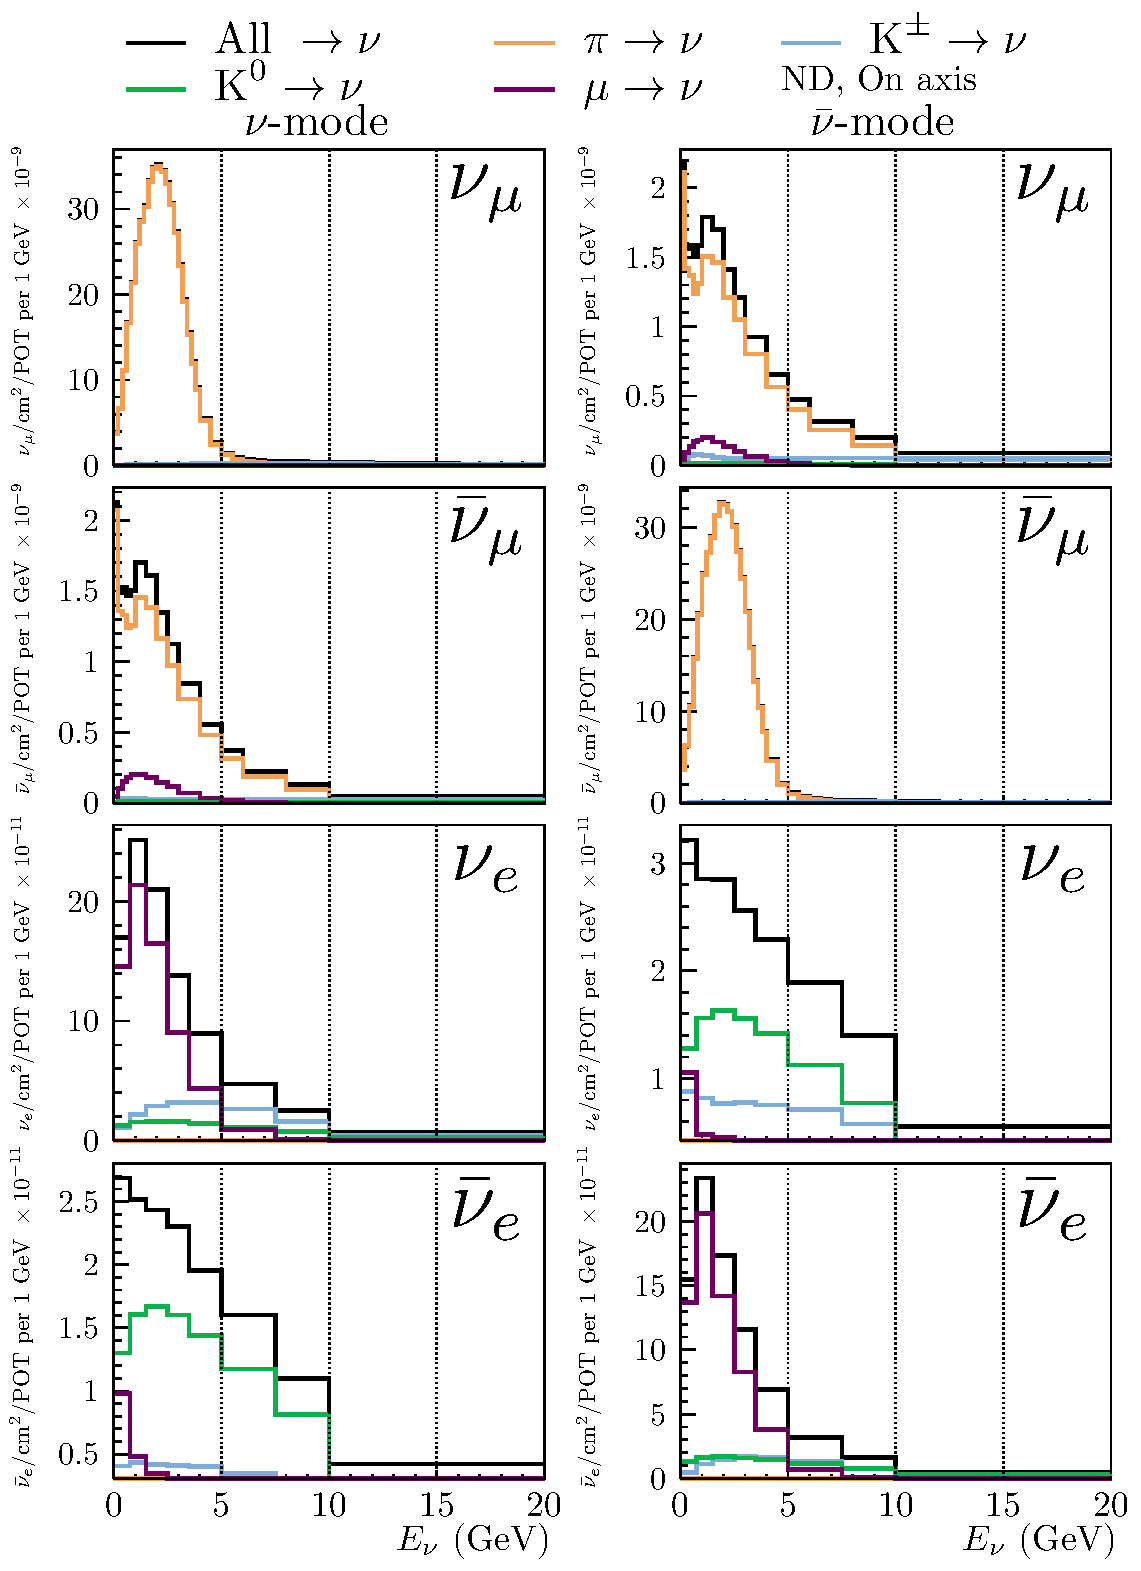
\includegraphics[width=0.95\textwidth]{plots/fluxpredcompvar/ND_HadronParentFluxComponents_0m_offaxis}
  \caption{DUNE Flux prediction averaged over a $6\times 3\times 5\,\textrm{m}^{3}$ volume on axis at 574 m from the proton beam target station. The left hand set of figures shows the prediction when running with positive (negative) horn polarity (\textit{i.e.} mostly matter (anti-matter)). The prediction of each neutrino species in each horn polarity configuration is separated by the particle species that decayed to produce a given neutrino.}
  \label{fig:flux_predictions__on_axis}
\end{figure}
\begin{figure}
  \centering
  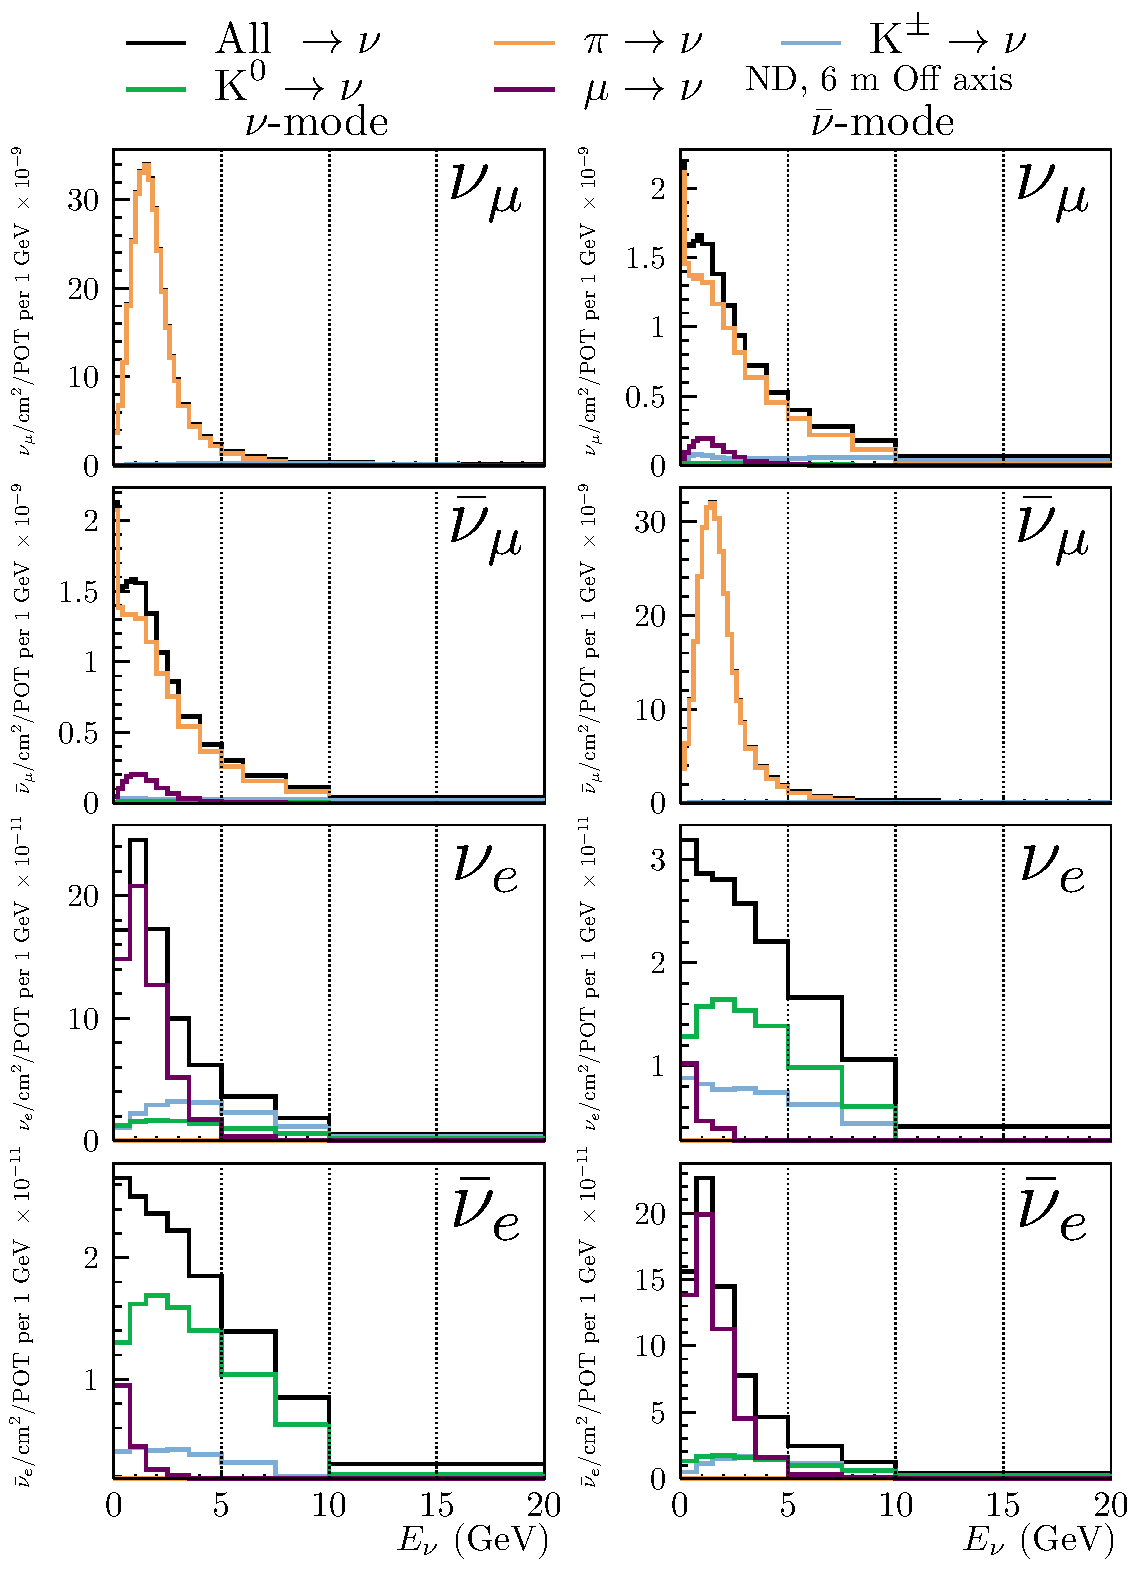
\includegraphics[width=0.95\textwidth]{plots/fluxpredcompvar/ND_HadronParentFluxComponents_6m_offaxis}
  \caption{DUNE Flux prediction averaged over a $6\times 3\times 5\,\textrm{m}^{3}$ volume 6 m laterally off beam axis at 574 m from the proton beam target station. The left hand set of figures shows the prediction when running with positive (negative) horn polarity (\textit{i.e.} mostly matter (anti-matter)). The prediction of each neutrino species in each horn polarity configuration is separated by the particle species that decayed to produce a given neutrino.}
\end{figure}
\begin{figure}
  \centering
  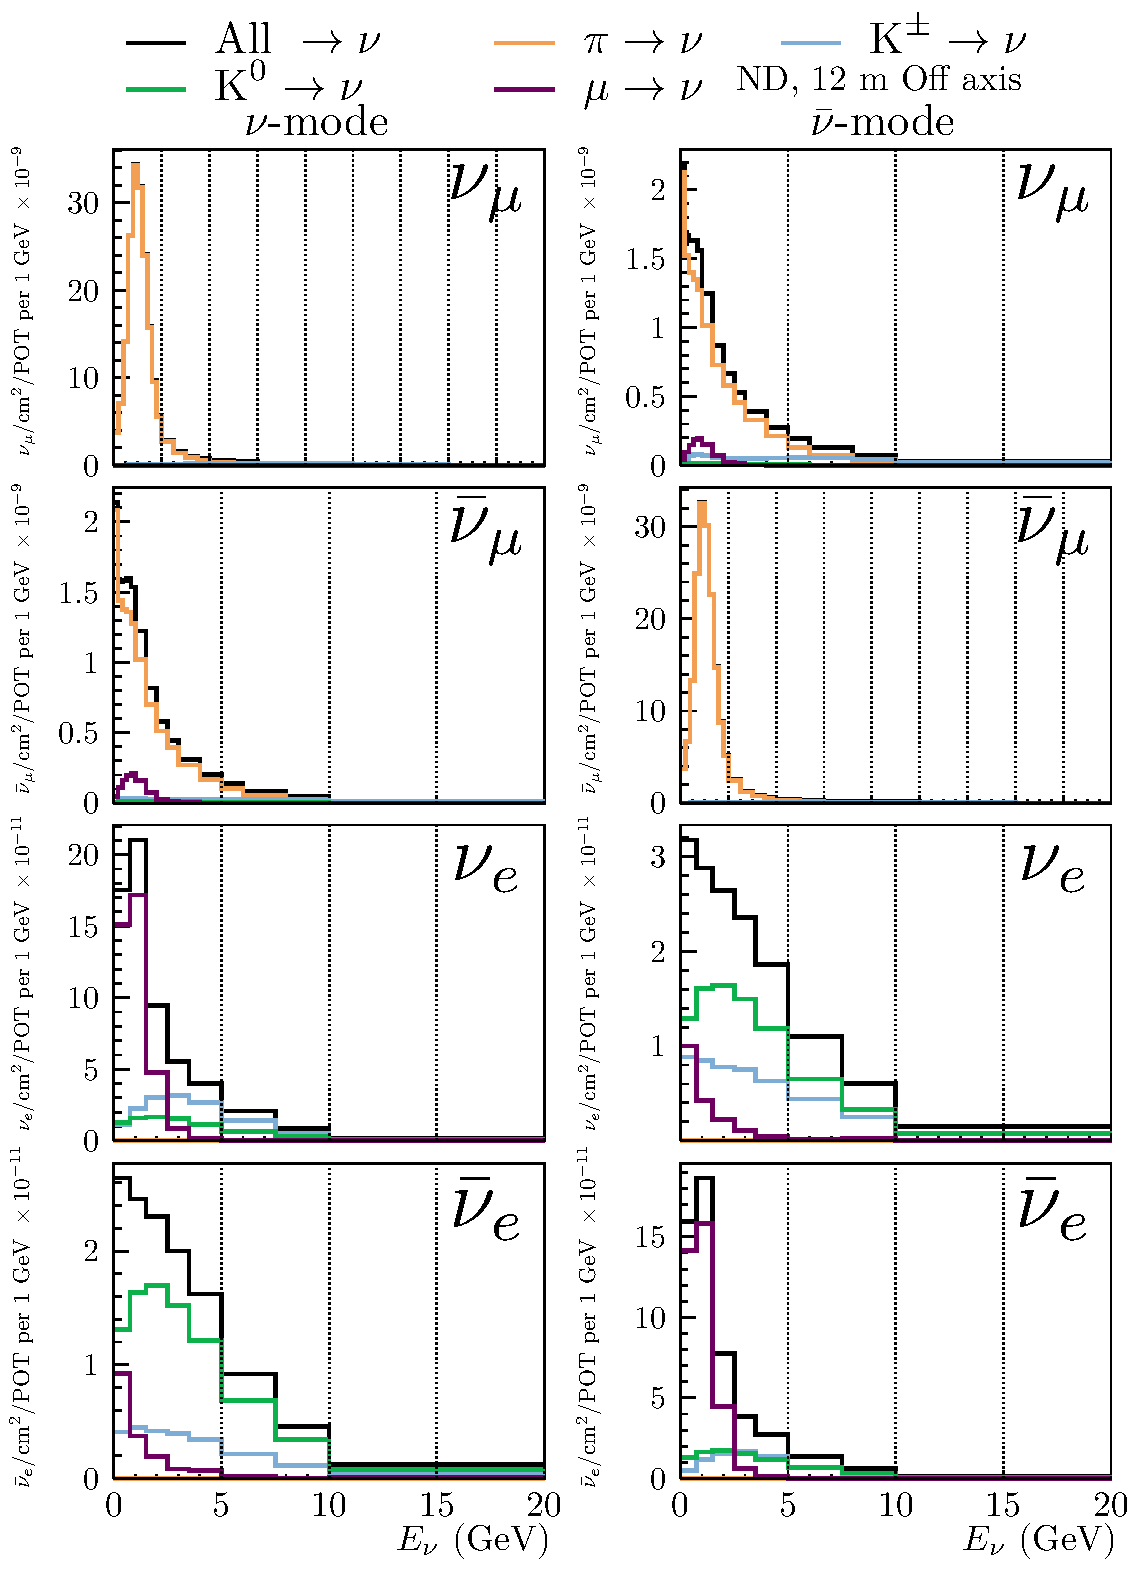
\includegraphics[width=0.95\textwidth]{plots/fluxpredcompvar/ND_HadronParentFluxComponents_12m_offaxis}
  \caption{DUNE Flux prediction averaged over a $6\times 3\times 5\,\textrm{m}^{3}$ volume 12 m laterally off beam axis at 574 m from the proton beam target station. The left hand set of figures shows the prediction when running with positive (negative) horn polarity (\textit{i.e.} mostly matter (anti-matter)). The prediction of each neutrino species in each horn polarity configuration is separated by the particle species that decayed to produce a given neutrino.}
\end{figure}
\begin{figure}
  \centering
  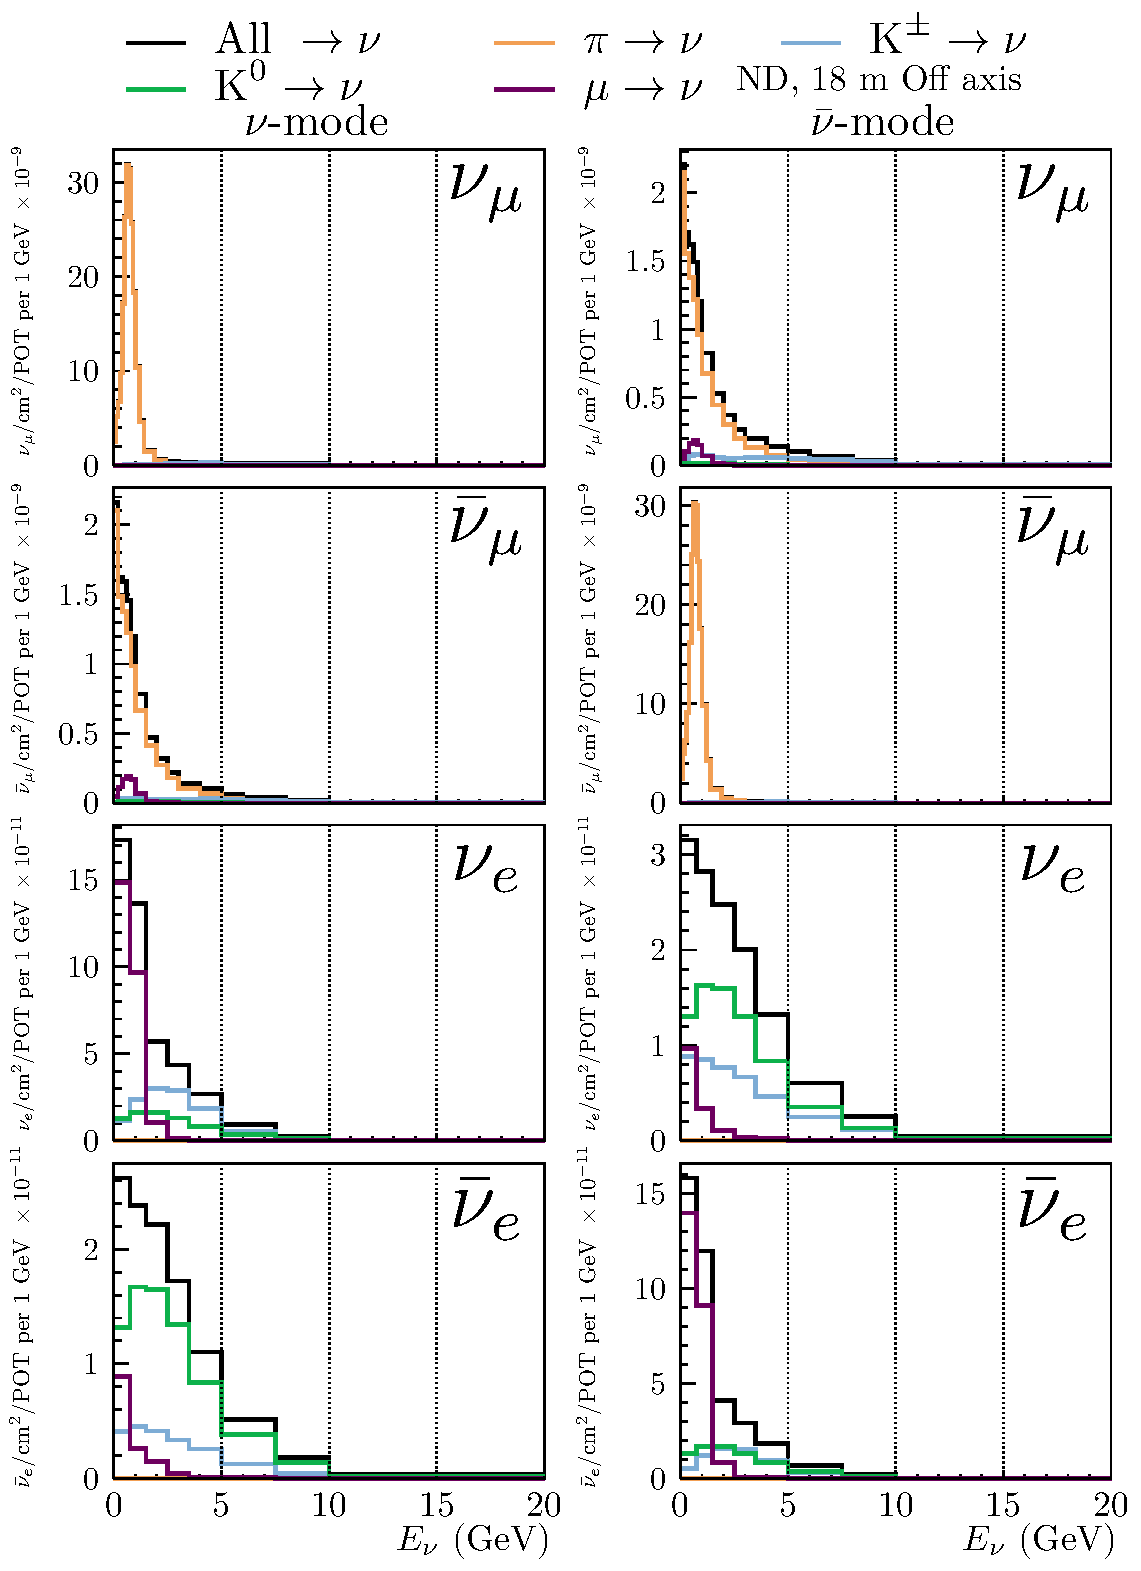
\includegraphics[width=0.95\textwidth]{plots/fluxpredcompvar/ND_HadronParentFluxComponents_18m_offaxis}
  \caption{DUNE Flux prediction averaged over a $6\times 3\times 5\,\textrm{m}^{3}$ volume 18 m laterally off beam axis at 574 m from the proton beam target station. The left hand set of figures shows the prediction when running with positive (negative) horn polarity (\textit{i.e.} mostly matter (anti-matter)). The prediction of each neutrino species in each horn polarity configuration is separated by the particle species that decayed to produce a given neutrino.}
\end{figure}
\begin{figure}
  \centering
  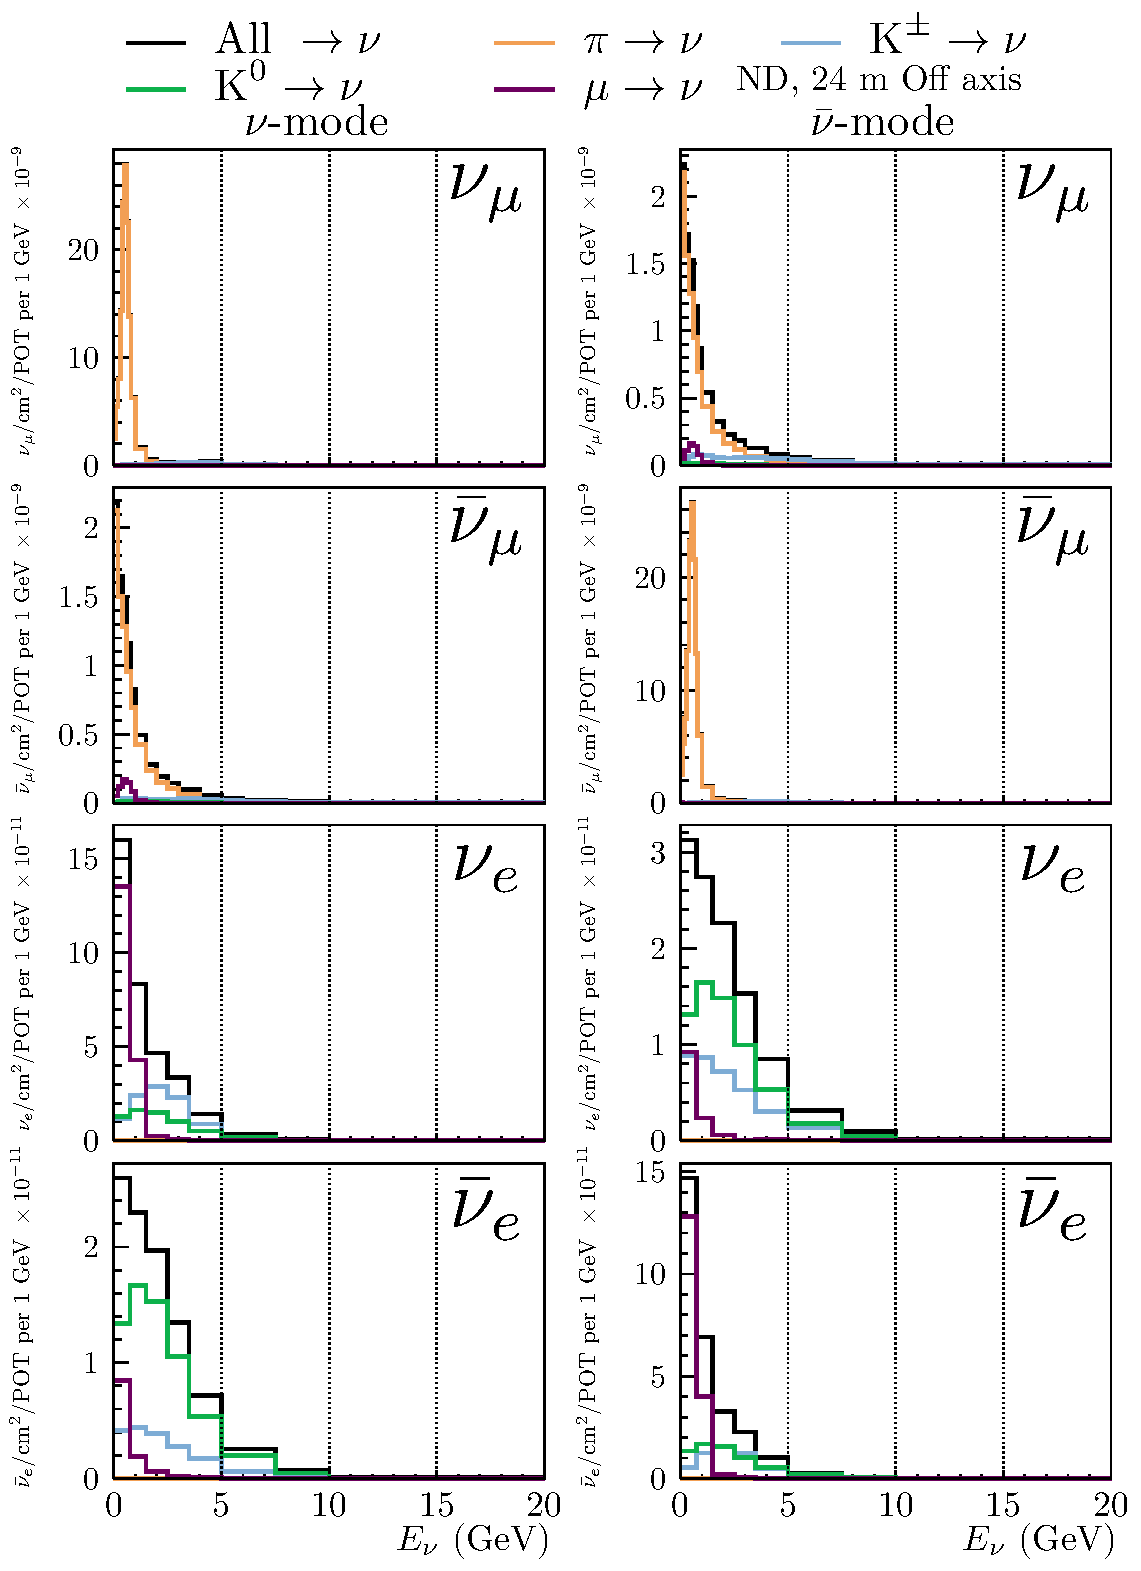
\includegraphics[width=0.95\textwidth]{plots/fluxpredcompvar/ND_HadronParentFluxComponents_24m_offaxis}
  \caption{DUNE Flux prediction averaged over a $6\times 3\times 5\,\textrm{m}^{3}$ volume 24 m laterally off beam axis at 574 m from the proton beam target station. The left hand set of figures shows the prediction when running with positive (negative) horn polarity (\textit{i.e.} mostly matter (anti-matter)). The prediction of each neutrino species in each horn polarity configuration is separated by the particle species that decayed to produce a given neutrino.}
\end{figure}
\begin{figure}
  \centering
  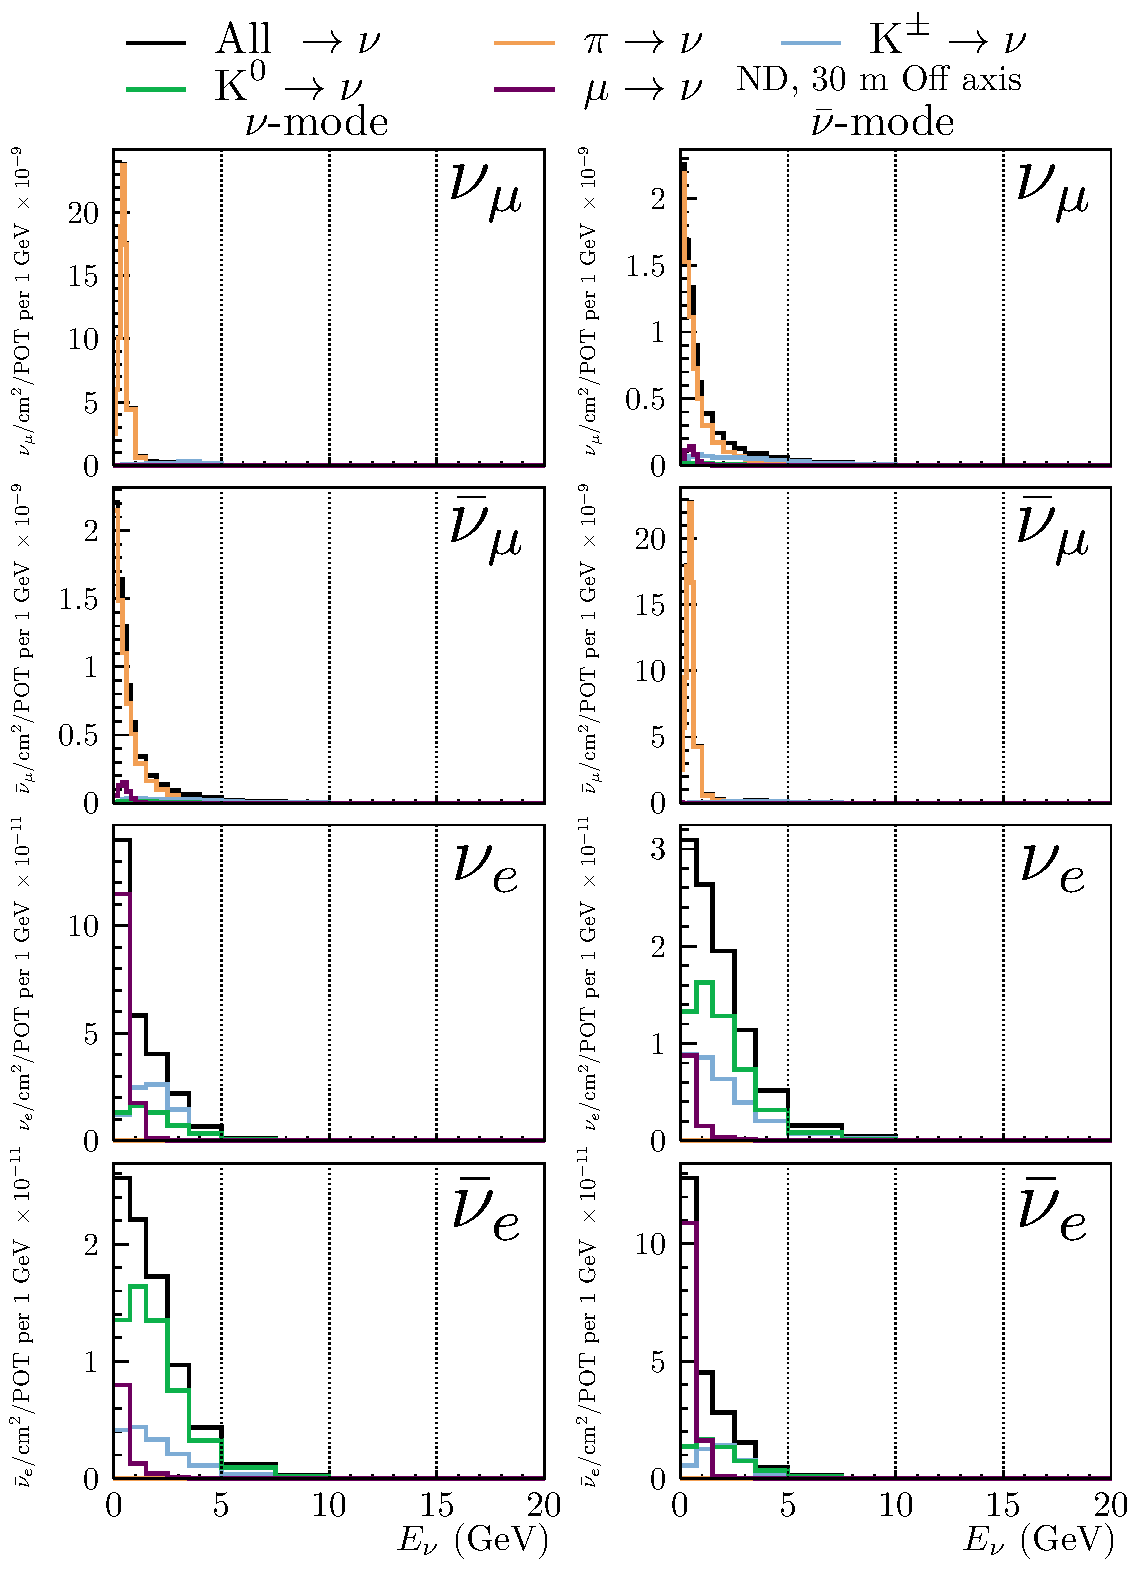
\includegraphics[width=0.95\textwidth]{plots/fluxpredcompvar/ND_HadronParentFluxComponents_30m_offaxis}
  \caption{DUNE Flux prediction averaged over a $6\times 3\times 5\,\textrm{m}^{3}$ volume 30 m laterally off beam axis at 574 m from the proton beam target station. The left hand set of figures shows the prediction when running with positive (negative) horn polarity (\textit{i.e.} mostly matter (anti-matter)). The prediction of each neutrino species in each horn polarity configuration is separated by the particle species that decayed to produce a given neutrino.}
  \label{fig:flux_predictions__off_axis}
\end{figure}

\begin{figure}
  \centering
  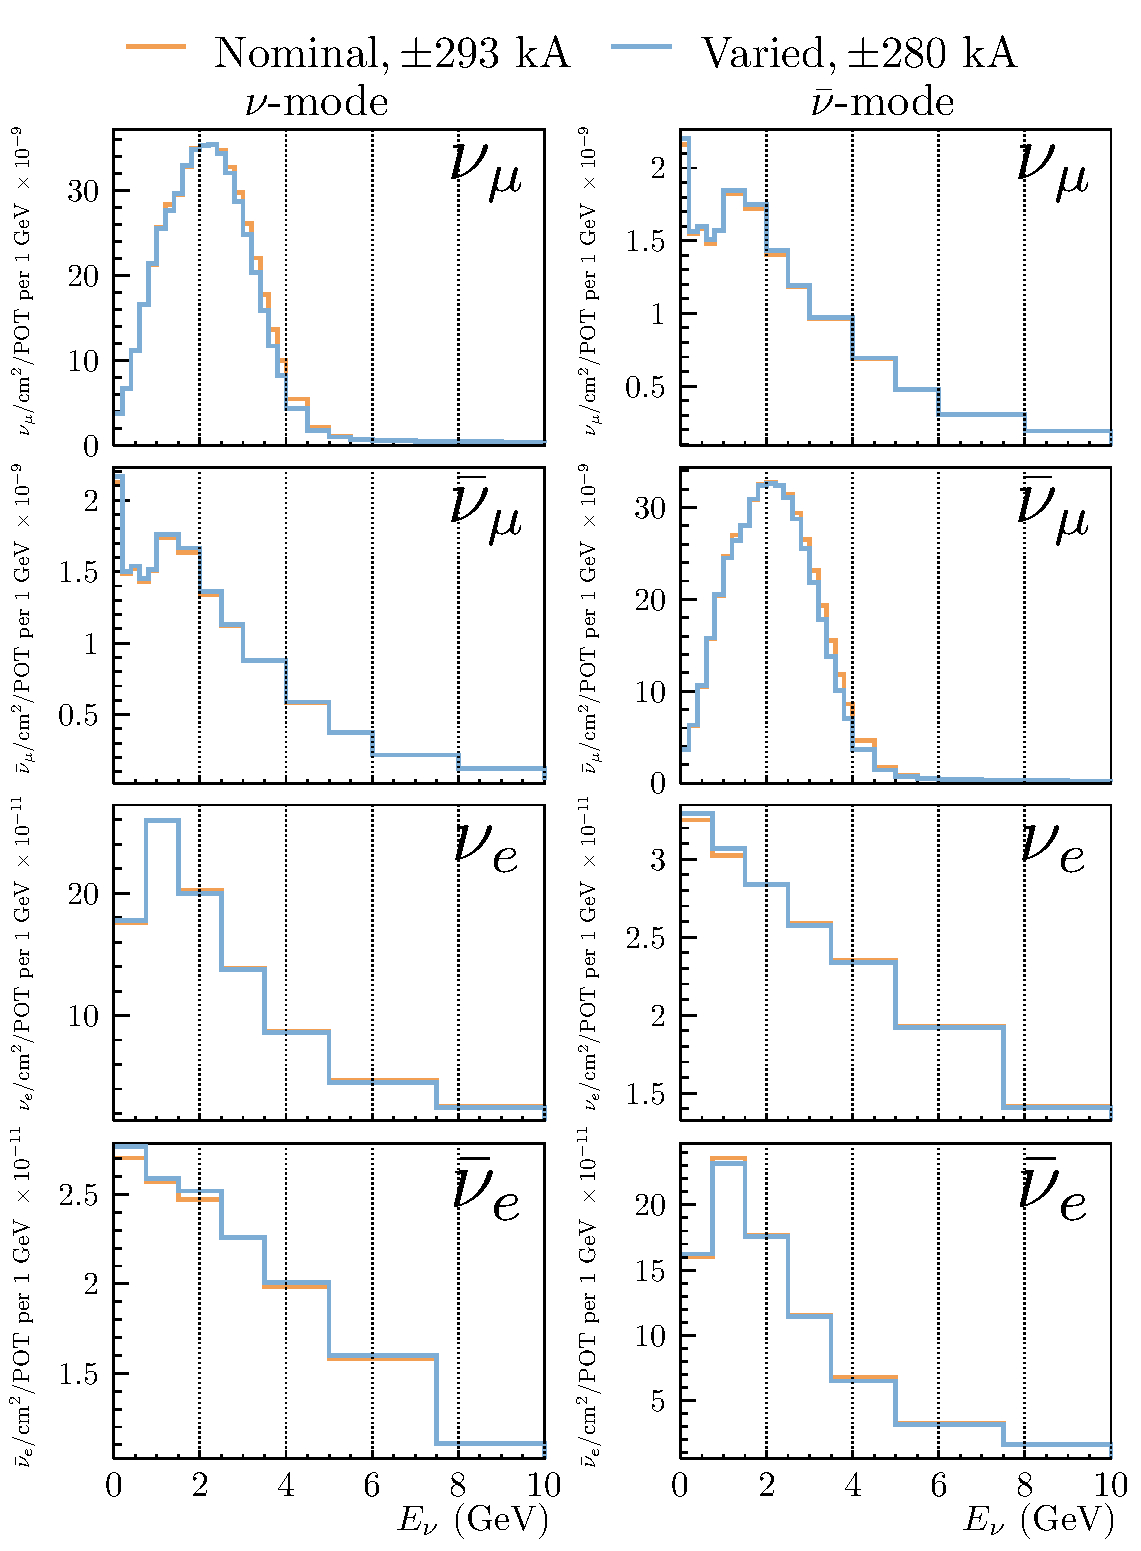
\includegraphics[width=0.95\textwidth]{plots/fluxpredcompvar/HornCurrentFluxPredictions}
  \caption{DUNE Flux prediction averaged over a $6\times 3\times 5\,\textrm{m}^{3}$ volume on axis at 574 m from the proton beam target station. The left hand set of figures shows the prediction when running with positive (negative) horn polarity (\textit{i.e.} mostly matter (anti-matter)). The prediction of each neutrino species in each horn polarity configuration is shown for the nominal horn current of $\pm293\, \textrm{kA}$ and for the PRISM special run current of $\pm280\, \textrm{kA}$.}
  \label{fig:flux_predictions__on_axis_lower_HC}
\end{figure}

\section{Methodology}

\subsection{Energy Binning}

As a primary driver for this re-analysis was the inclusion of an error analysis for off axis positions at the near detector site, the energy binning needs to be treated somewhat carefully. This is for two main reasons, firstly, if the energy or off axis binnings are too fine, then the number of bins becomes large and standard analysis techniques to use flux constraints become impractical (matrix inversion and decomposition). Secondly, at further off axis positions, the flux peaks at a much lower energy than on axis ($0.6$ GeV vs. $\sim 2.3$ GeV), this means that if an error analysis is performed with a uniform energy binning as a function of off axis angle, then MC statistical noise at far off axis positions and higher energies can dominate and produce problematic results.

As a result, the analysis was performed using a custom histogram class, \texttt{TH2Jagged}, which subclasses the \texttt{TH2} from \texttt{ROOT}. It allows for 2D rectangular histogram with one axis defined as a function of the other axis. In this case, the energy binning is a function of the off-axis angle binning. As using custom classes is somewhat fiddly, the final output will not rely on the analyzer having access to this class. There are three binnings used in this analysis: one for the 'right sign' muon neutrino ($\nu_{\mu}$ in $\nu$-mode and $\bar{\nu}_{\mu}$ in $\bar{\nu}$-mode) , one for the 'wrong sign' muon neutrino ($\bar{\nu}_{\mu}$ in $\nu$-mode and $\nu_{\mu}$ in $\bar{\nu}$-mode), and a third for all electron-type neutrinos (which constitute $\sim 1\% $ of the total flux in any configuration). The binning definitions can be seen in Fig.~\ref{fig:binning}.

\begin{figure}
  \centering
  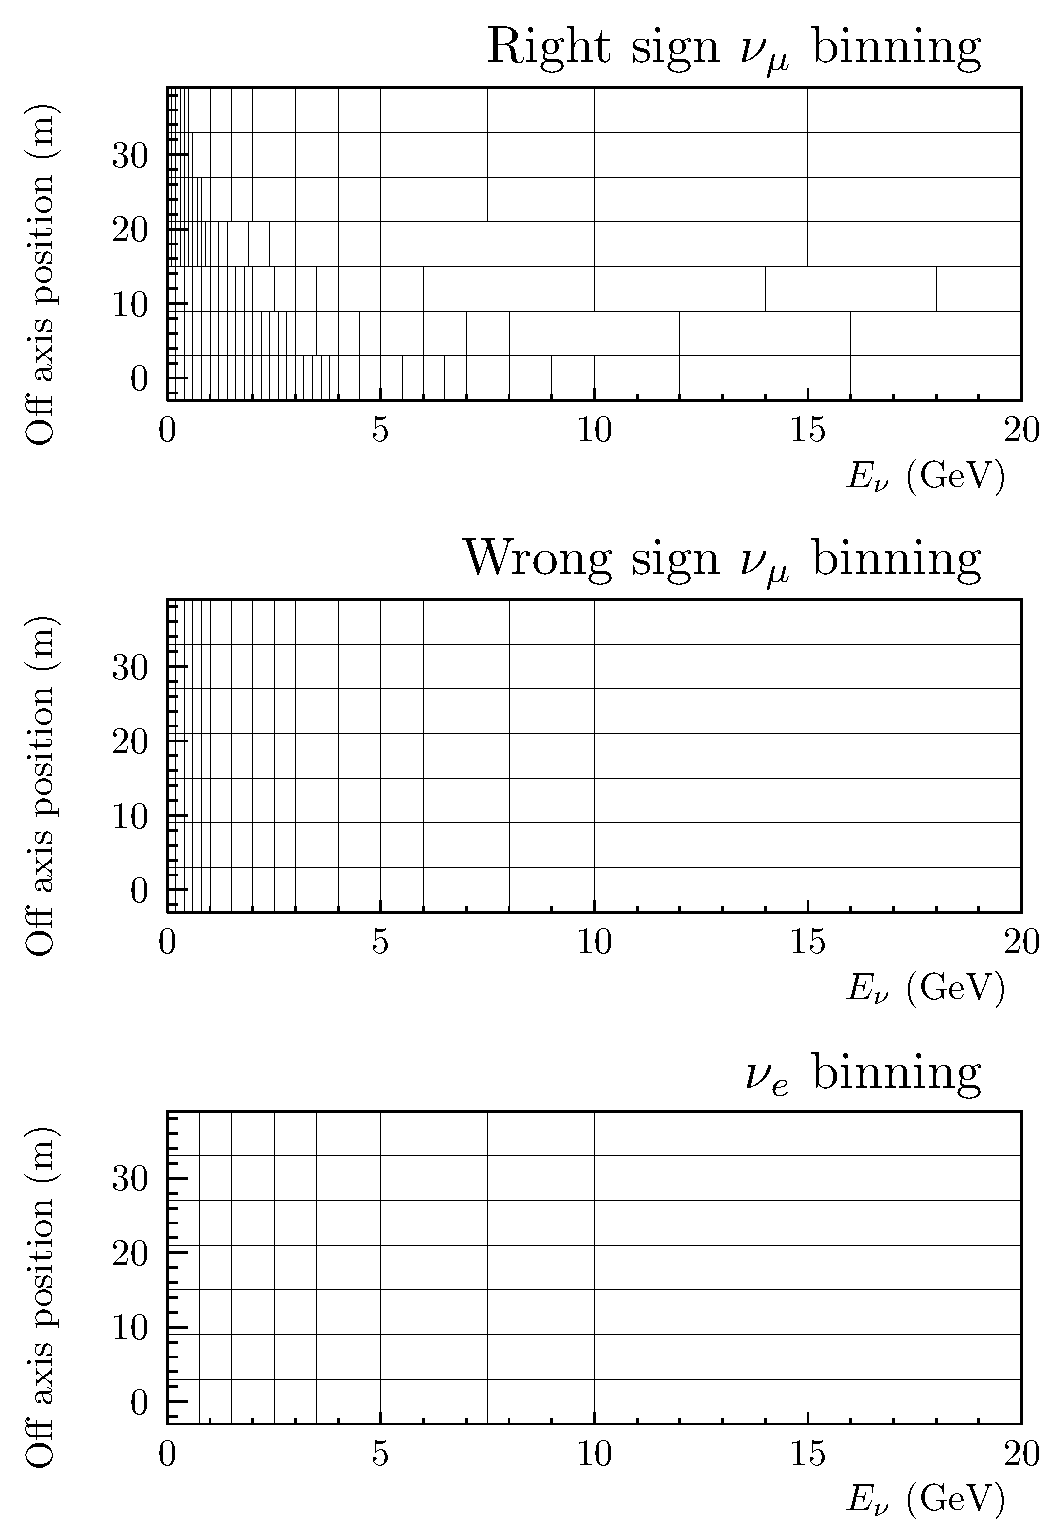
\includegraphics[width=0.95\textwidth]{plots/Binning}
  \caption{The species, off axis, and energy binning that was used in this analysis.}
  \label{fig:binning}
\end{figure}

\subsection{Error determination}
\label{sec:methodology__error_determination}

The methodology for error propagation follows the previous notes closely.
There are 3 types of systematic variation used in this analysis: firstly, discrete variations where only a single shifted prediction is made and compared to the 'nominal' prediction to determine the magnitude of the effect. These could come from non-continuous variations, but practically in this analysis, all discrete shifts are continuous systematic variations of which only a single point is sampled. For such a variation the relevant component of the total error matrix is determined in the usual way by:
\begin{equation}\mathbf{C} = \left(\vec{v}-\bar{n}\right)\left(\vec{v}-\bar{n}\right)^{\mathrm{T}}\label{eqn:covmx},\end{equation}
where $\vec{v}$ is the shifted prediction and $\bar{n}$ is the nominal prediction.

It is worth noting here that a prediction, $\vec{x}$, may contain any number of sub-predictions produced under the same beam conditions, \textit{i.e.} two horn polarities with 4 neutrino species for each of six near and and one far detector volumes is the standard prediction configuration used in this analysis. The error analysis does not care about any specifics of the binning as long the final error calculated for the $i$-th component of a prediction $\vec{\phi}$ can be correctly re-associated to the correct beam-mode, species, detector volume, and energy bin when diseminating the final uncertainties.

The second type of systematic variation is one where more than one sample along a single degree of freedom is made, and each must be included simultaneously in the error analysis. An example of this is the uncertainty on the vertical position of the second horn, for which one prediction at $+0.5 mm$ and one at $-0.5 mm$ was used. Here a polynomial is fit to the shifted predictions in each bin, this follows the treatment in \cite{}, but here the polynomial order is always the same as the number of varied samples (i.e. one less than the number of points to be fit). The fitted polynomial is then evaluated at $+1$ in each bin, producing a varied prediction, $\vec{v}$. Eqn~\ref{eqn:covmx} is again used to produce the error matrix component from an uncertainty of this type.

The final type is one where a larger number of samples are taken from a higher dimensional space of nuisance parameters. The canonical and only uncertainties treated this way are the hadron production uncertainties. The underlying parameters are binned cross-section normalizations for a large number of interactions that GEANT can simulate during the proton and daughter particle propagation through the target and horn geometry. There are far too many parameters to treat individually like the focussing and alignment errors. Instead flux predictions for some number of random\footnote{These random throws are constrainted by (possibly correlated) priors informed by hadron production experiments. See \texttt{PPFX} notes\cite{} for more details.} throws within this ($\mathcal{O}\left(700\right)$ dimension) parameter space are calculated and used to asses the correlated uncertainties from hadron production errors. The component matrix is then formed by the generalization of Eqn~\ref{eqn:covmx} to $N$ samples:
\[\mathbf{C} = 1/N\sum^{i=0}_{i<N} \left(\vec{v_{i}}-\bar{n}\right)\left(\vec{v_{i}}-\bar{n}\right)^{\mathrm{T}}\label{eqn:covmxN}.\]


\section{Uncertainties Used}

\label{sec:uncertainties_used}
Table~\ref{tbl:uncertdefn} contains the systematic variations used. The 'type' of each variation as defined in \S~\ref{sec:methodology__error_determination} can be determined by the number of listed variations. Note that each of these sources of error are treated as independent. The \texttt{g4lbne} macro files used for each systematically varied prediction should be distributed with this note, the 'Name' column corresponds to the macro file used with the exception of the 'PPFX' variations which are calculated by reweighting the nominal prediction.

\begin{table}
\centering
\begin{tabular}{l|l|l}
Name & Category & Variations \\
\hline
PPFX & Hadron production & 100 throws about \texttt{PPFX} CV tune \\
\hline
DecayPipeRadius & Focussing & +10 cm \\
WaterLayer & Focussing & +0.5 mm \\
HornCurrent & Focussing & +3, -3 kA \\
TargetDensity & Focussing & +1.8, -1.8 \% \\
\hline
Horn1XShift & Horn Alignment & +3,+0.5, -0.5, -3 mm\\
Horn2XShift & Horn Alignment & +0.5, -0.5 mm \\
Horn1YShift & Horn Alignment & +0.5, -0.5 mm \\
Horn2YShift & Horn Alignment & +0.5, -0.5 mm \\
\hline
BeamTheta & Beam Alignment & 0.07 mrad tilt \\
BeamThetaPhi & Beam Alignment & 0.07 mrad tilt and $90^{\circ}$ rotation about $\hat{z}$ \\
BeamSigma & Beam Alignment & +0.1, -0.1 mm \\
BeamOffsetX & Beam Alignment & +0.45, -0.45 mm \\
\end{tabular}
\caption{The systematic variations used in this analysis.}
\label{tbl:uncertdefn}
\end{table}

\section{Error Propagation}

\subsection{Error Matrices}

The total on-axis-only error matrices from all sources of error described in \S~\ref{sec:uncertainties_used} can be seen in Fig.~\ref{fig:covmat}. The corresponding correlation matrix can be seen in Fig.~\ref{fig:corrmat}. This matrix is only shown for the on axis near detector position as including the off axis stops shown elsewhere in this document brings the total bin count to $\mathcal{O}\left(1000\right)$. If correlated uncertainties at off axis stops are needed, it is recommended that the eigenvector/eigenvalue technique of error propagation is used as then no large matrix handling is required at analysis time.

\paragraph{N.B.} At the time of writing the non-PPFX uncertainties had not been evaluated for the $280\,\textrm{kA}$ special run and so are assumed to be identical to the nominal run. The only difference therefor between the 'Near Detector' and the 'Special ND run' sections of the matrices is the hadron production uncertainty contribution.

\begin{figure}
  \centering
  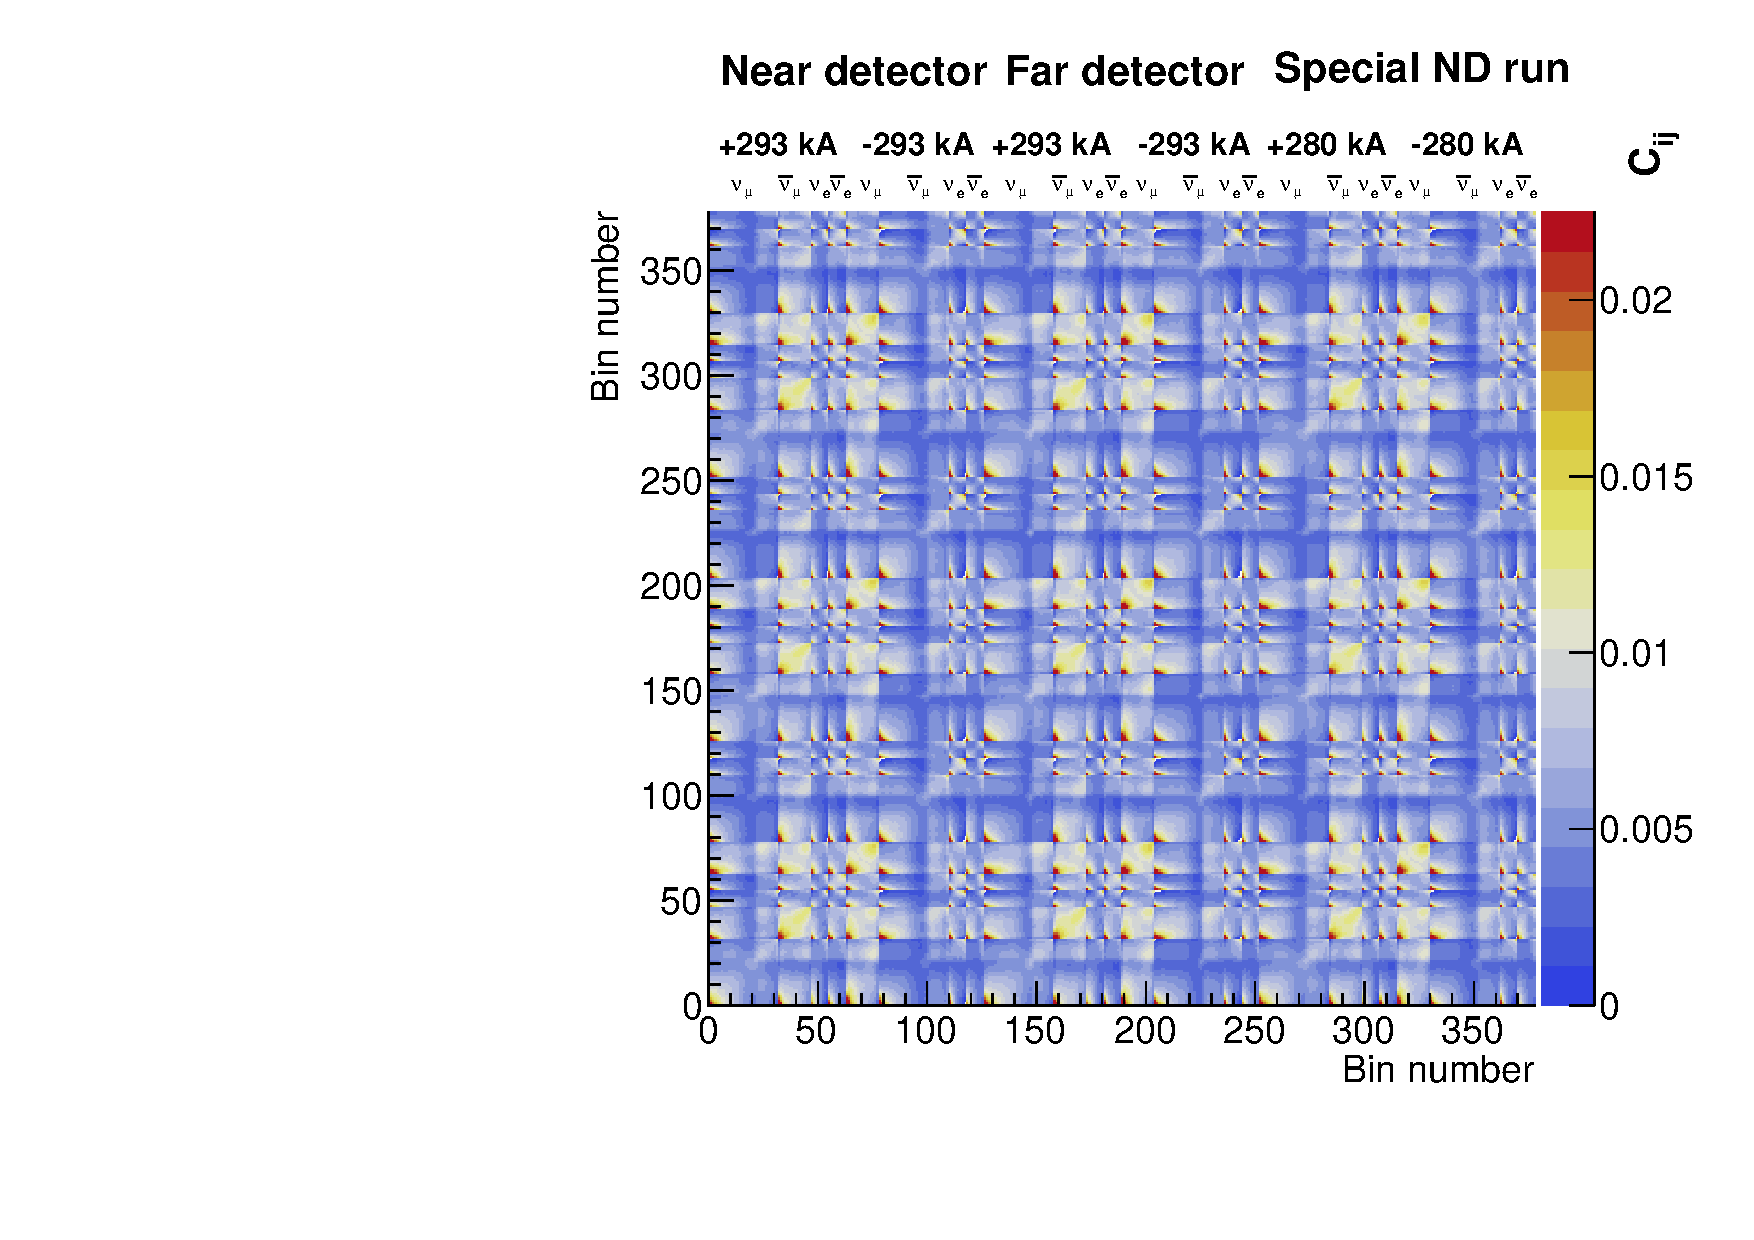
\includegraphics[width=0.95\textwidth]{plots/mats/ErrorMatrices_covmat}
  \caption{The total error (covariance) matrix describing the correlated neutrino flux prediction uncertainties across neutrino energies, between two horn polarities, two detector volumes, and four neutrino species, and including a special lower horn current near detector run. \textbf{N.B.} For the special horn current run, the non-PPFX uncertainties were not re-evaluate, and so are assumed fractionally the same as the nominal horn current runs.}
  \label{fig:covmat}
\end{figure}

\begin{figure}
  \centering
  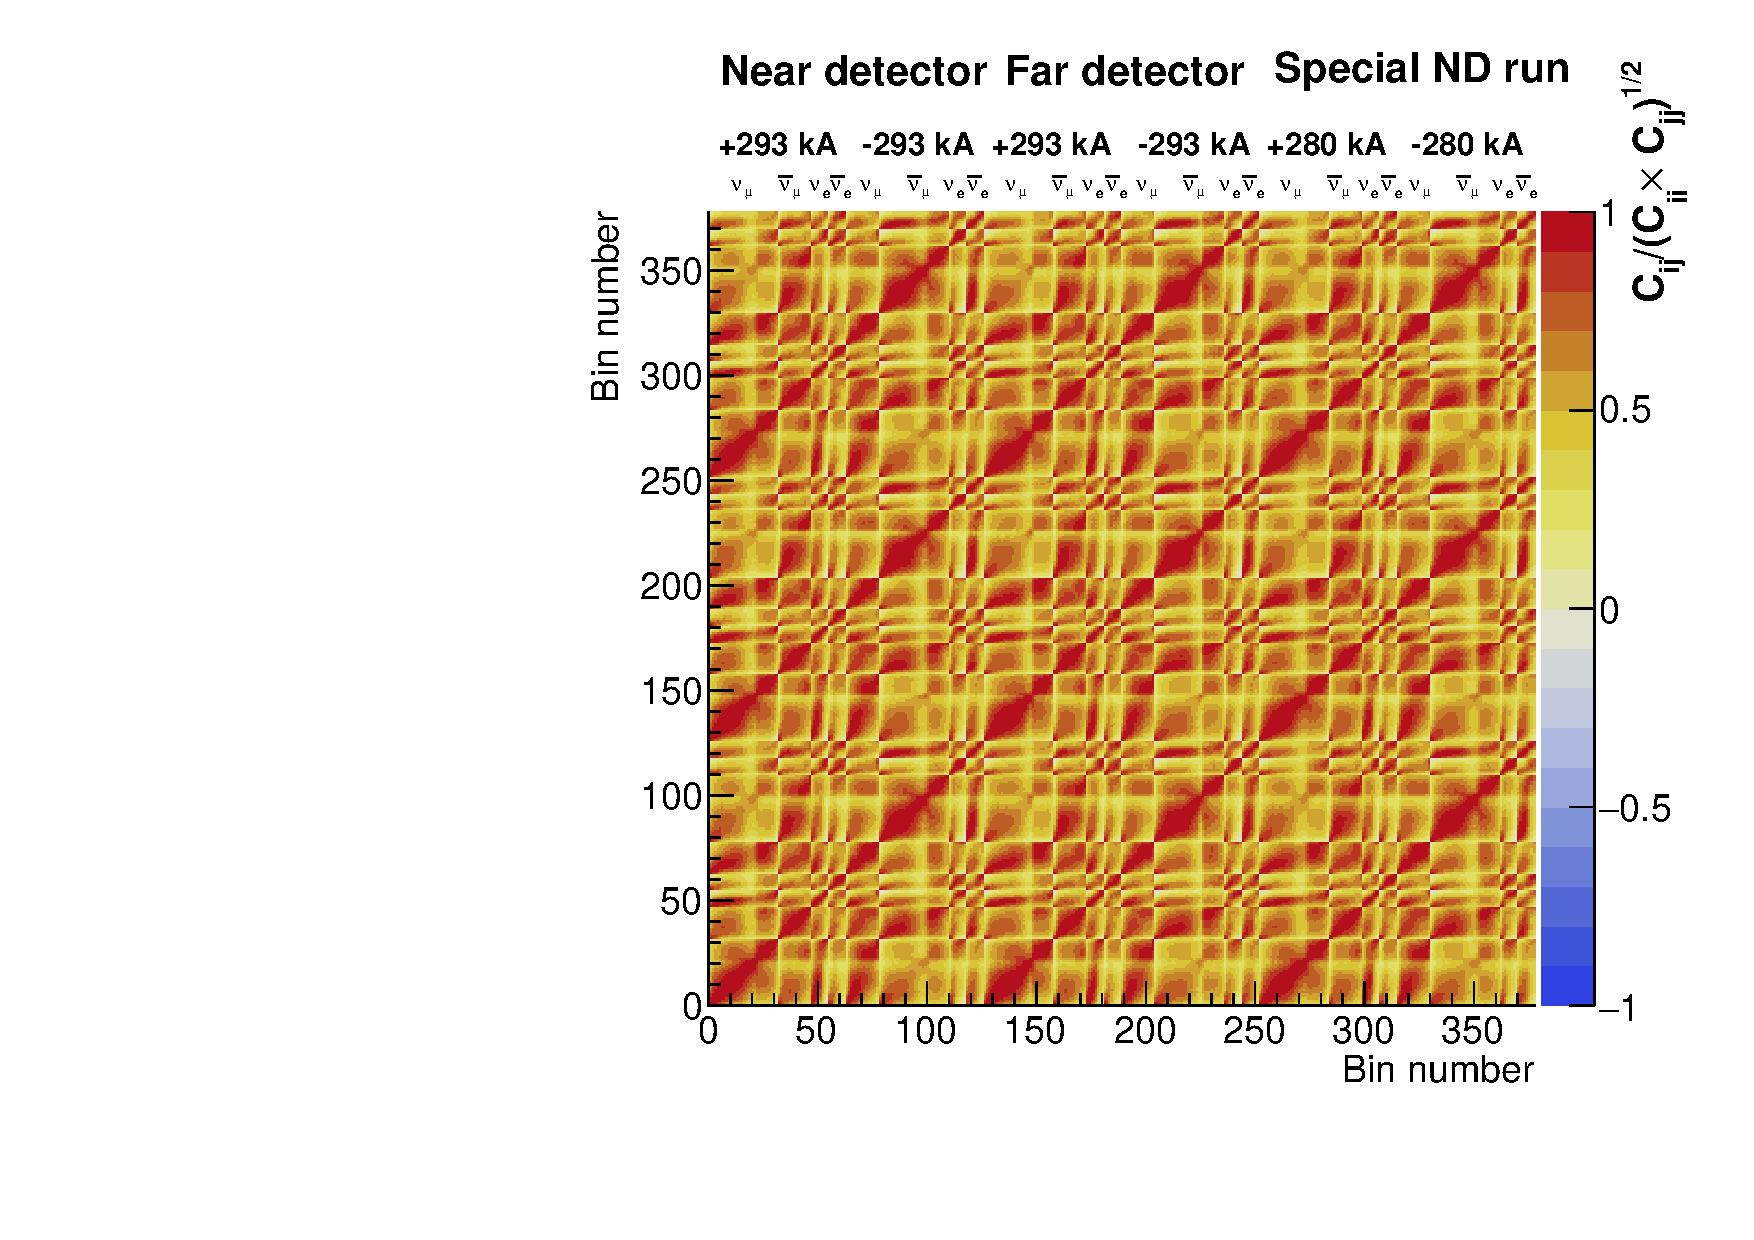
\includegraphics[width=0.95\textwidth]{plots/mats/ErrorMatrices_corrmat}
  \caption{The correlation matrix describing the correlated neutrino flux prediction uncertainties across neutrino energies, between two horn polarities, two detector volumes, and four neutrino species, and including a special lower horn current near detector run. \textbf{N.B.} For the special horn current run, the non-PPFX uncertainties were not re-evaluate, and so are assumed fractionally the same as the nominal horn current runs.}
  \label{fig:corrmat}
\end{figure}

\subsection{Analyzer Usage}

The error matrix shown in Fig.~\ref{fig:covmat} can be incorporated into analyses in a number of ways. There are two common ways. Firstly, each beam mode (including special horn current runs), species, energy bin in which the uncertainties are calculated introduces a nuisance parameter to the analysis. The value of these nuisance parameters control the relative probability (weight) for events produced by true neutrinos that fall within the corresponding bin. The matrix can then be used to form a penalty term like,
\[\chi^{2}_\textrm{pen}\left(\textbf{p}\right)=\textbf{p}\mathbf{C}^{-1}\textbf{p}^\mathrm{T},\]
where, $\textbf{p}$ is the vector of nuisance parameter values and $\mathbf{C}$, is the total error matrix. The nature of beamline uncertainties results in constraints that are often strongly correlated across beam modes, neutrino species, and energy bins. As a result, this method can prove problematic for gradient descent minimization. This method neccessarily introduces one parameter per beam mode, neutrino species, and energy bin, this number cannot be reduced without losing granularity. For finely binned uncertainties as a function of off axis position at the near detector, this number can be prohibitively large, $\mathcal{O}\left(1000\right)$.

The second method is conceptually similar but mechanically slightly more involved and can be used to side-step the two problems highlighted for the first method. The total number of varied predictions that went into the analysis was presented here was 120 (100 PPFX universes and 20 other variations), however, for even on-axis-only and coarse energy binning the number of columns and rows in $\mathbf{C}$ is likely to be $\mathcal{O}\left(200\right)$. The matrix $\mathbf{C}$ can be diagonalized and then only the most important $k$ eigenvectors and values used in error propagation---where $k<120$, as the eigenvectors corresponding to smaller eigenvalues will be composed of MC statistical and floating point precision noise. This decomposition is equivalent to a rotation from a basis of beam mode, neutrino species, and energy bin normalizations to an effective basis that describes the correlated constraint described by $\mathbf{C}$ across each simultaneously.

\subsection{Matrix Decomposition}

The \texttt{Spectra}\footnote{https://spectralib.org/} and \texttt{Eigen}\footnote{http://eigen.tuxfamily.org} packages are used to perform a 'brute force' eigen-decomposition of the error matrices where only the first $k$ eigen vectors and values are computed for an $n\times{}n$ square matrix, $k<n$. The \texttt{spectra} technique is attractive because performing more 'traditional' eigen-decomposition (such as those offered by \texttt{ROOT}) requires the full $n$ eigen vectors and values to be computed, which can be computationally very costly. If we only need the first 120 eigen vectors and values from a $1000\times{}1000$ error matrix, \texttt{Spectra} takes many orders of magnitude less time to calculate them than a full decomposition in \texttt{ROOT}. The distribution of eigen values for the matrix shown in Fig.~\ref{fig:covmat} can be seen in Fig.~\ref{fig:evdist}. We can check the total variance that remains after truncating the number of eigen vectors by comparing the sum of square eigenvalues and the trace of the original matrix. If we only kept $k=100$ eigen vectors and values, the total remaining variance would be 99.9995\% of the original matrix, for $k=30$ this becomes 98\%.

\begin{figure}
  \centering
  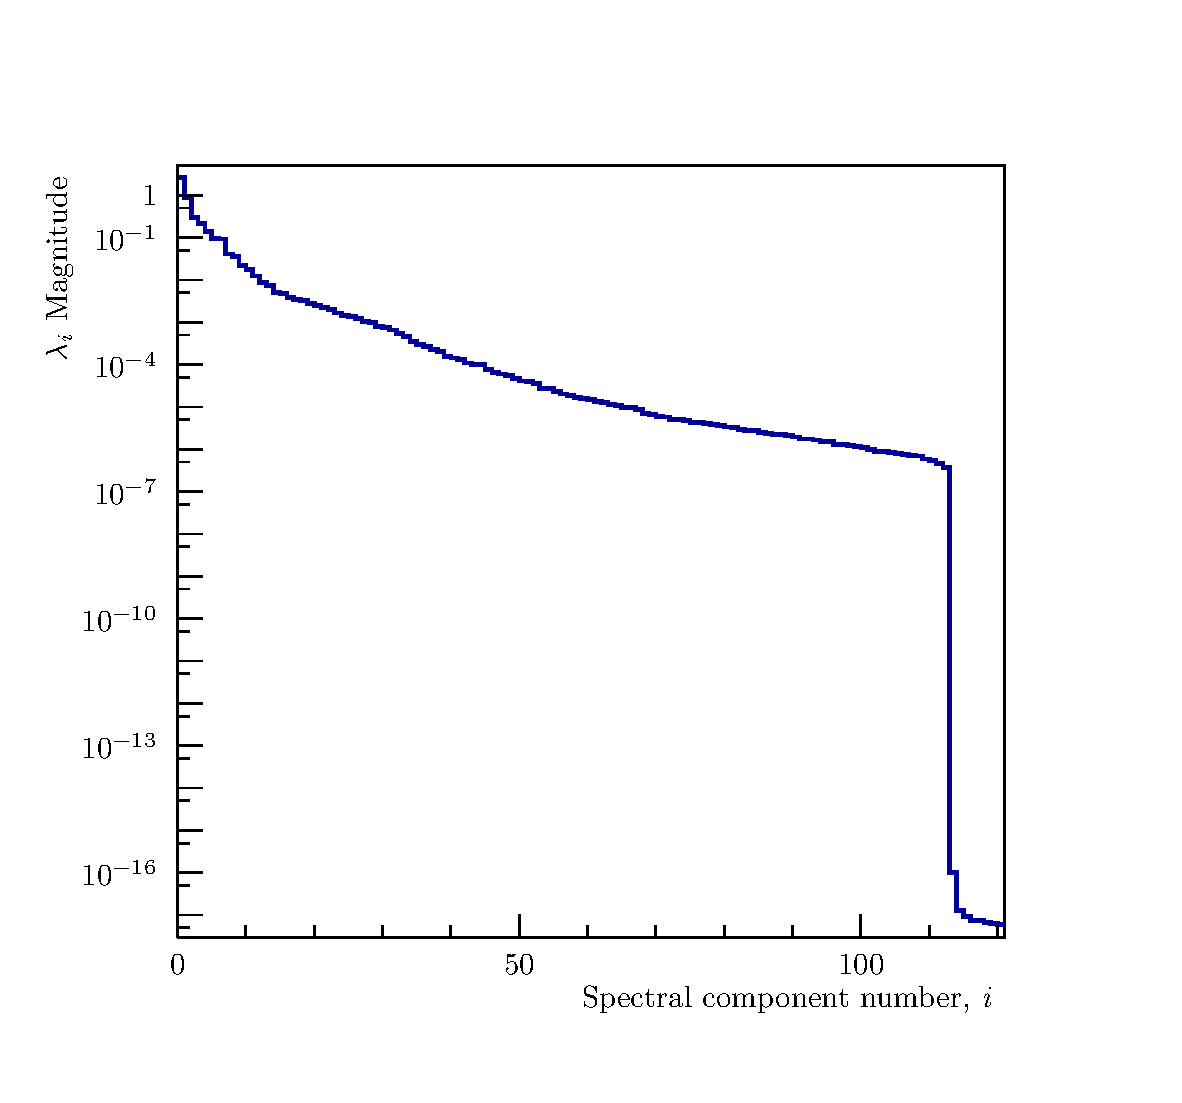
\includegraphics[width=0.95\textwidth]{plots/allpca_evs}
  \caption{The distribution of eigen values from the decompositon of Fig.~\ref{fig:covmat}. It can be seen that by the 30th eigen value, the extra contribution to the total variance of each extra eigen vector is less than 0.1\% of the first. The sharp drop at $i=110$ is a result of the underlying number of degrees of freedom in the matrix, the drop to $10^{-16}$ corresponds to the relative precision of \texttt{double}floating point values.}
  \label{fig:evdist}
\end{figure}

The freedom corresponding to the five most important eigen vectors is shown in Fig.~\ref{fig:evfreedom}. This corresponds to only 20\% of the total variance of the original matrix, but is illustrative of how each eigen vector parameter effects a correlated change across both detectors, both beam modes, each species, and all energies. This can be naturally extended to include the off axis positions needed for the PRISM analysis. Figs.~\ref{fig:evfreedom_offaxis_c0}--\ref{fig:evfreedom_offaxis_c2} show the near detector freedom from the three most important eigen vectors, for each species and beam mode.
Fig.~\ref{fig:evfreedom_offaxis_total} shows the total uncertainty for the off axis near detector.

\begin{figure}
  \centering
  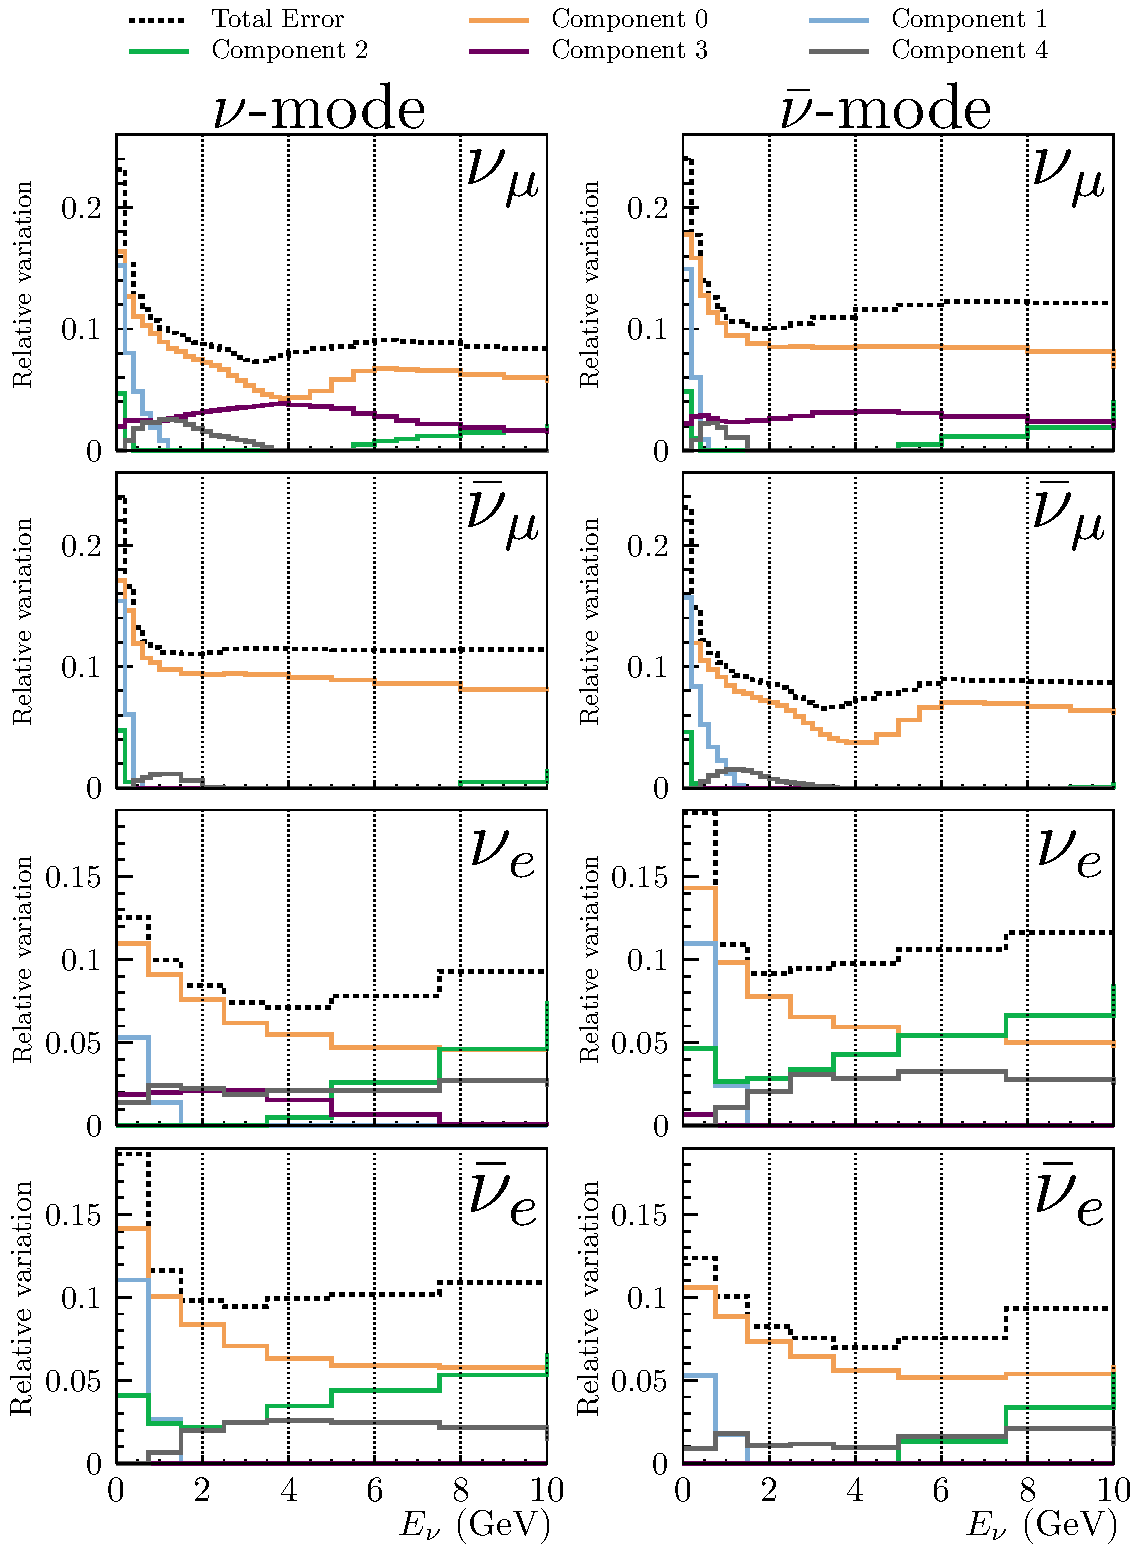
\includegraphics[width=0.95\textwidth]{plots/EvUncerts_allpca}
  \caption{The five most important eigen vectors in the decomposition of the on axis only total flux error matrix---only the projection into the near detector flux predictions are shown. Here the flux predictions are averaged over the on axis flux volume.}
  \label{fig:evfreedom}
\end{figure}

\begin{figure}
  \centering
  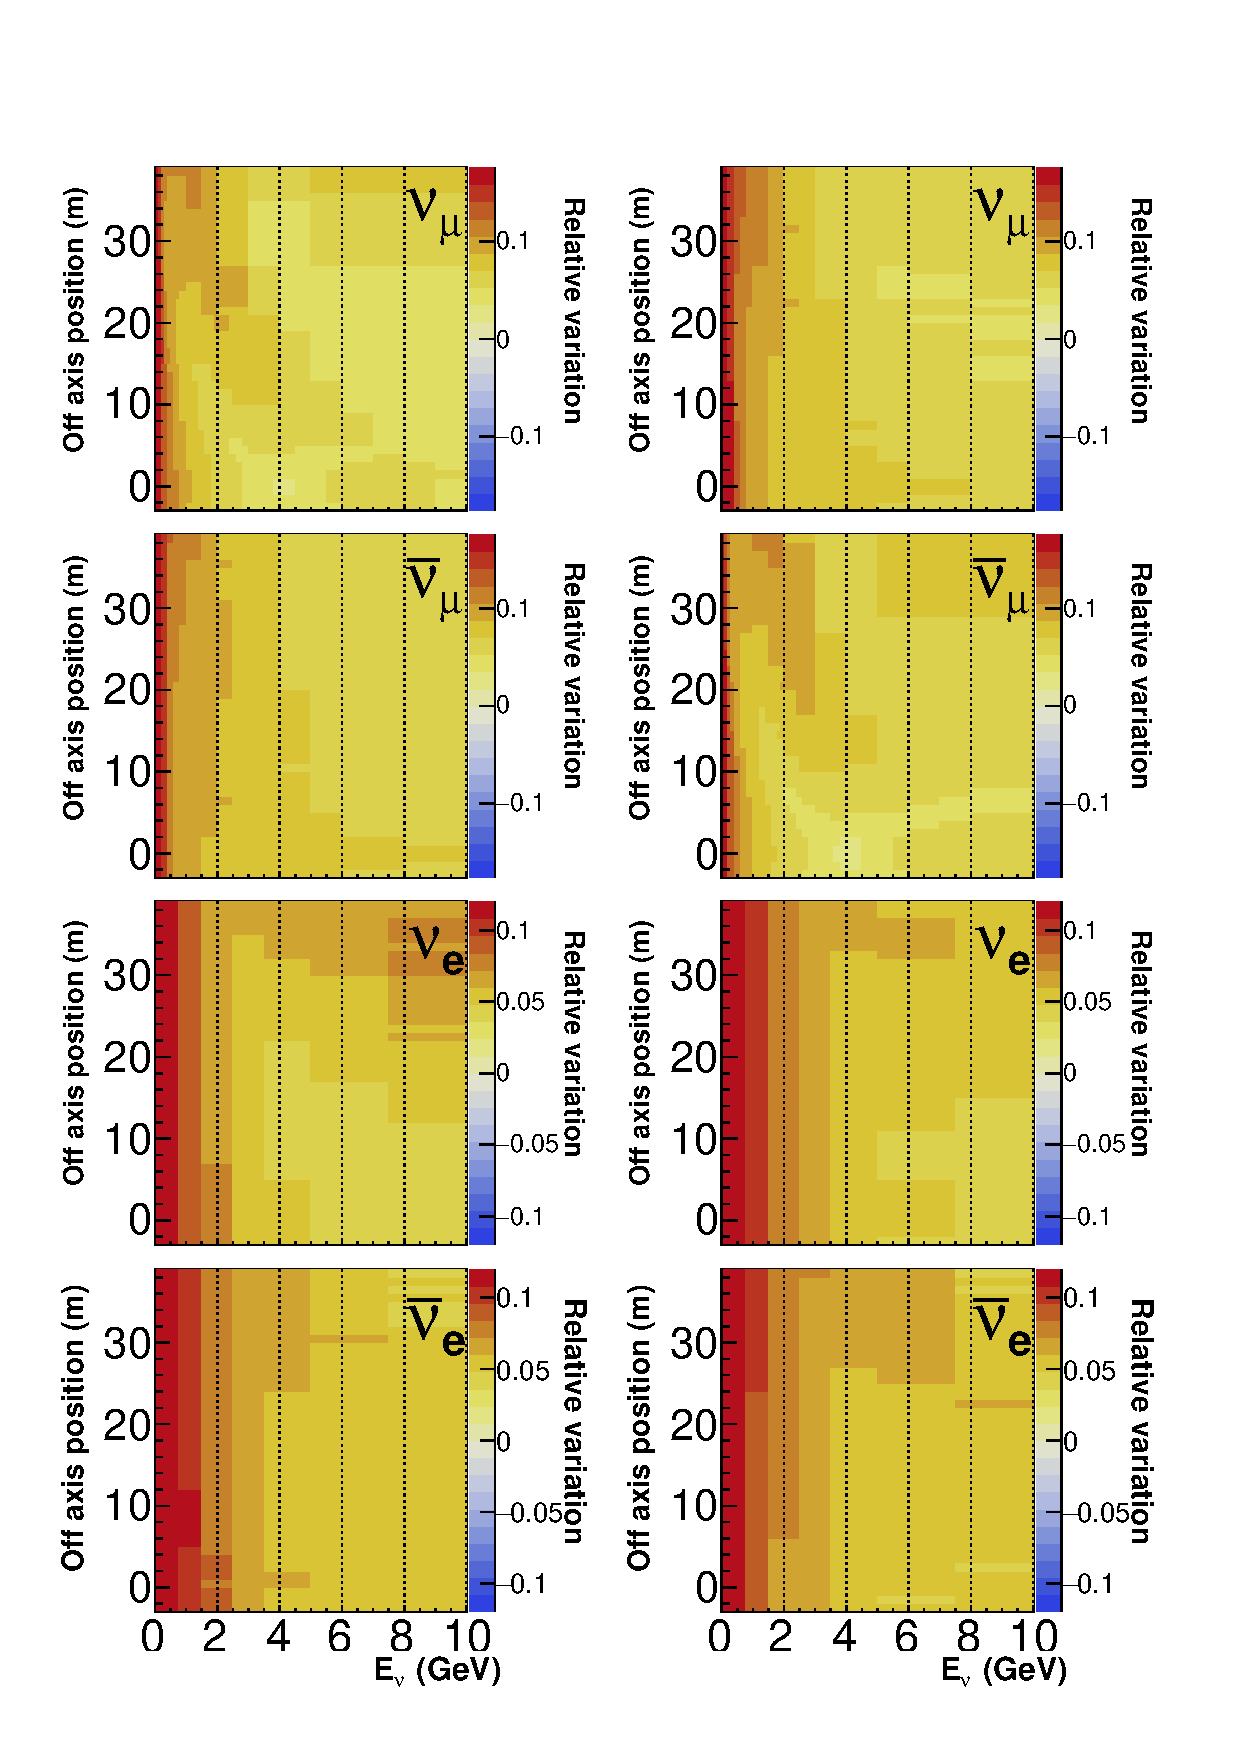
\includegraphics[width=0.95\textwidth]{plots/EvUncerts_offaxis_component_0}
  \caption{The most important eigen vector in the decomposition of the total flux error matrix---including off axis near detector flux volumes---only the projection into the near detector flux predictions are shown. Here the flux predictions are averaged over the on axis flux volume. \textbf{N.B} that the preferred method of propagation only eigen-decomposes the hadron production error matrix, and as such this figure does not represent a recommended degree of freedom.}
  \label{fig:evfreedom_offaxis_c0}
\end{figure}

\begin{figure}
  \centering
  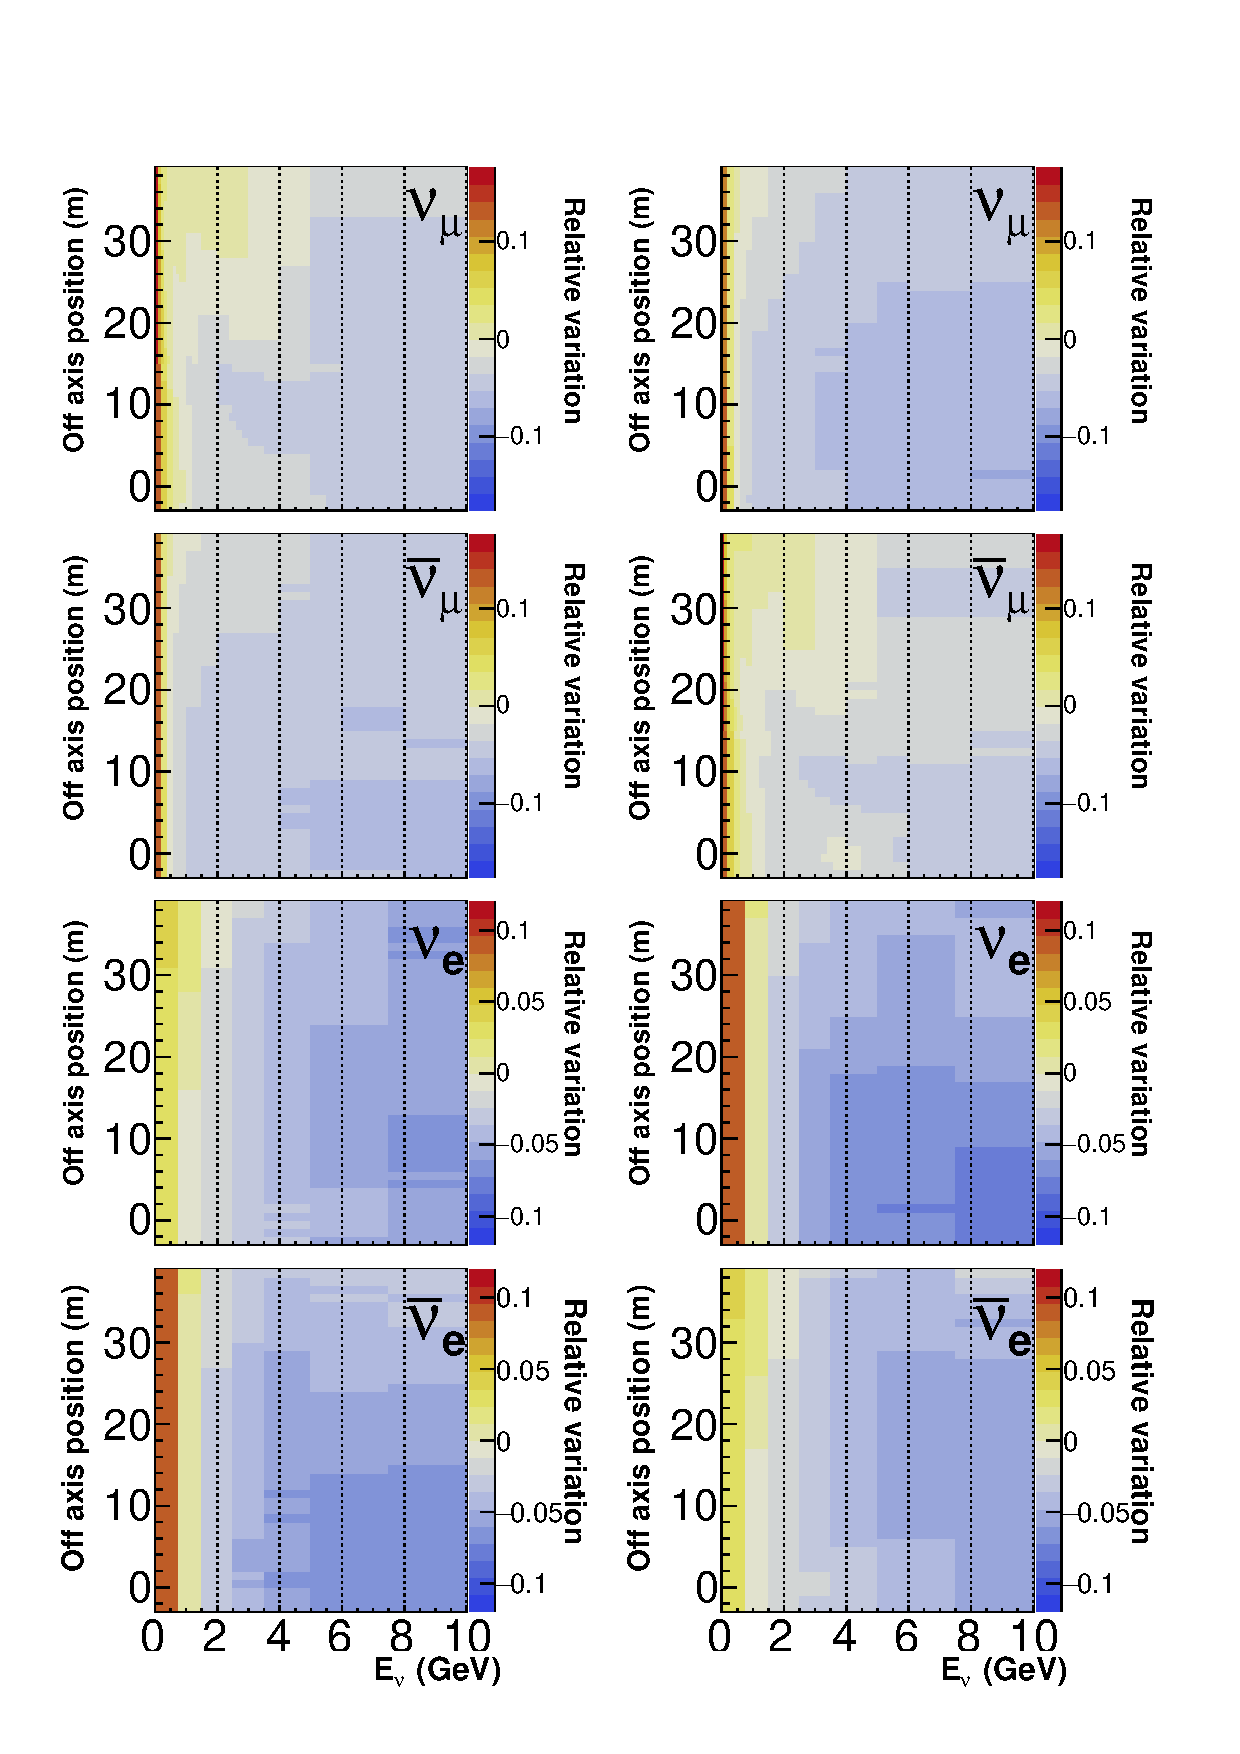
\includegraphics[width=0.95\textwidth]{plots/EvUncerts_offaxis_component_1}
  \caption{The second most important eigen vector in the decomposition of the total flux error matrix---including off axis near detector flux volumes---only the projection into the near detector flux predictions are shown. Here the flux predictions are averaged over the on axis flux volume. \textbf{N.B} that the preferred method of propagation only eigen-decomposes the hadron production error matrix, and as such this figure does not represent a recommended degree of freedom.}
  \label{fig:evfreedom_offaxis_c1}
\end{figure}

\begin{figure}
  \centering
  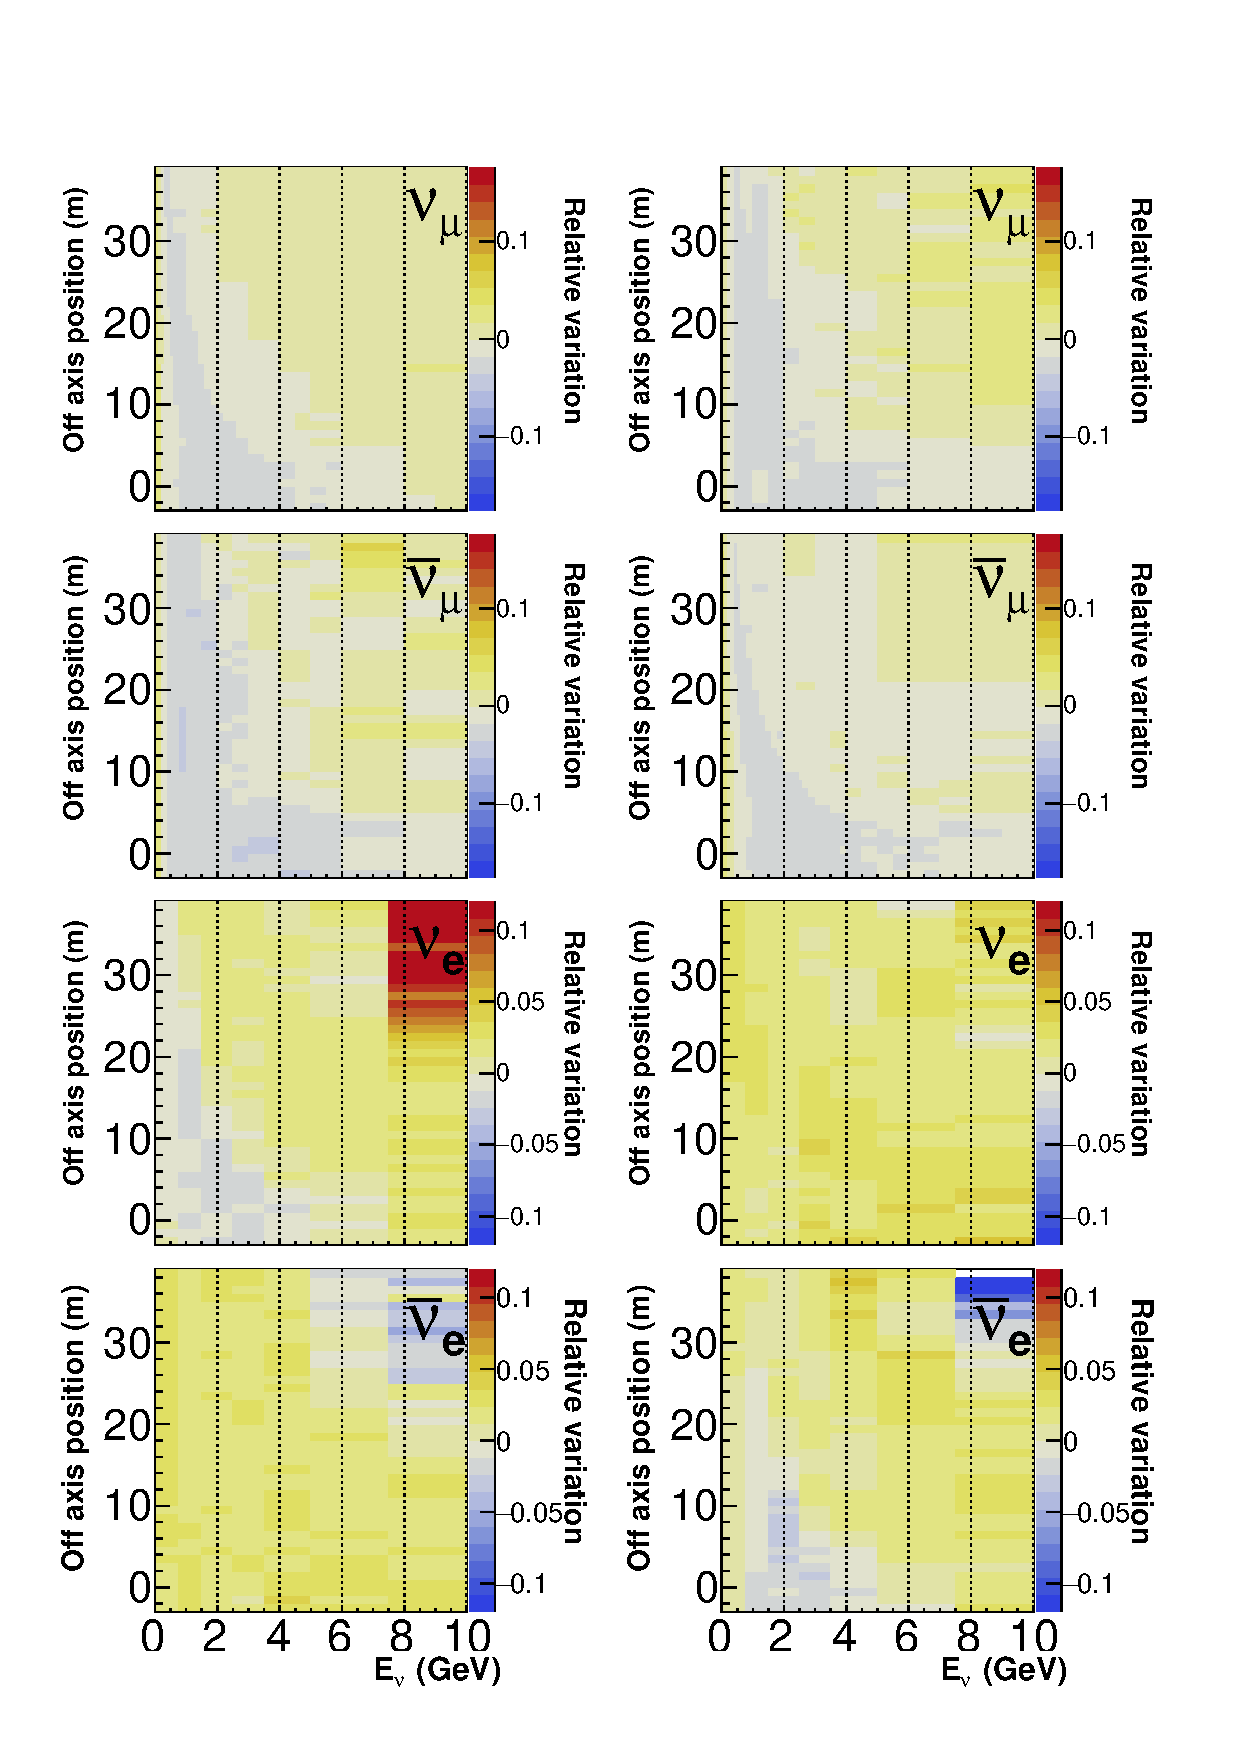
\includegraphics[width=0.95\textwidth]{plots/EvUncerts_offaxis_component_2}
  \caption{The third most important eigen vector in the decomposition of the total flux error matrix---including off axis near detector flux volumes---only the projection into the near detector flux predictions are shown. Here the flux predictions are averaged over the on axis flux volume. \textbf{N.B} that the preferred method of propagation only eigen-decomposes the hadron production error matrix, and as such this figure does not represent a recommended degree of freedom.}
  \label{fig:evfreedom_offaxis_c2}
\end{figure}

\begin{figure}
  \centering
  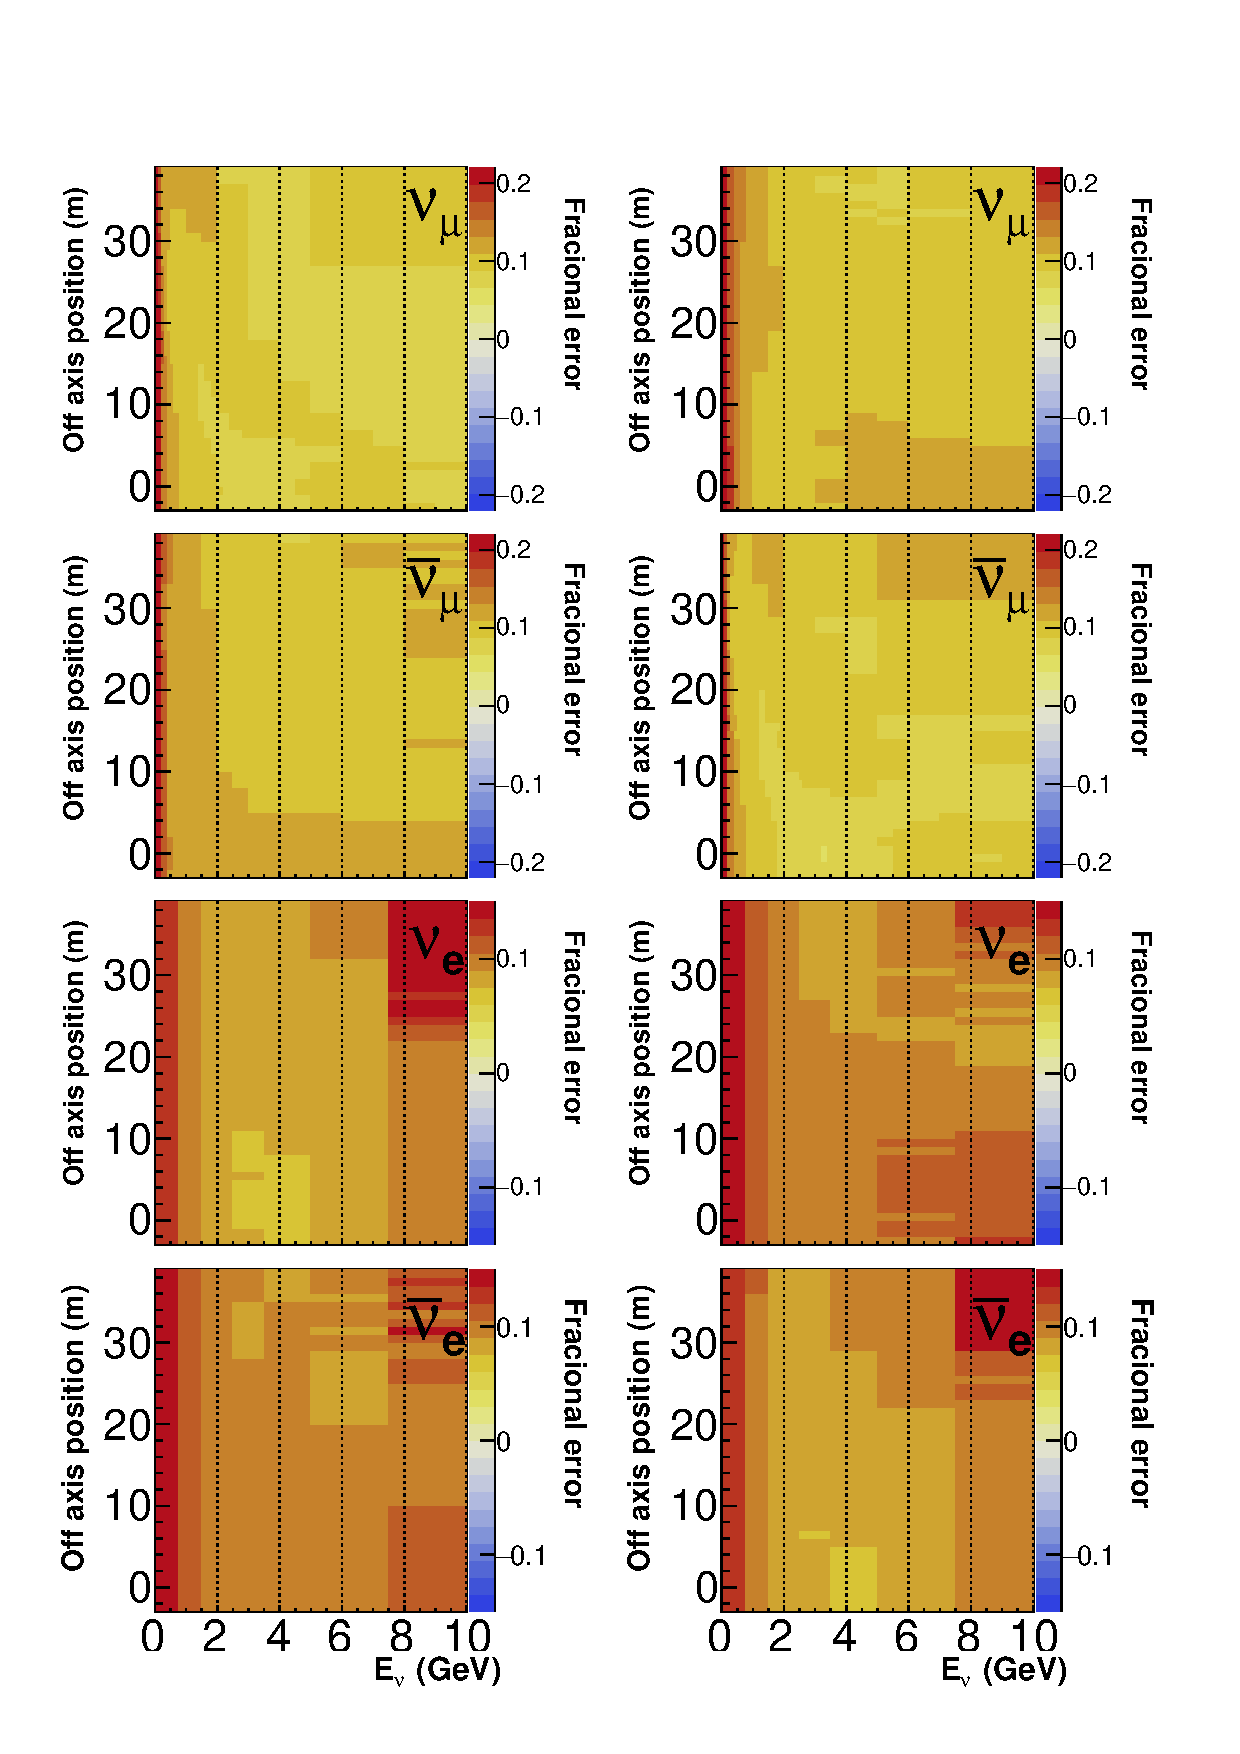
\includegraphics[width=0.95\textwidth]{plots/EvUncerts_offaxis_total}
  \caption{The total fractional uncertainty on the near detector flux predictions---including off axis near detector flux volumes. Here the flux predictions are averaged over the on axis flux volume.}
  \label{fig:evfreedom_offaxis_total}
\end{figure}

It is worth noting here that for all varied predictions apart from the \texttt{PPFX} universes, a separate MC simulation was run. This means that in regions that are less well populated, higher energies at further near detector off axis positions, or the predictions for non-dominant neutrino species, bin-by-bin it can be hard to distinguish MC statistical noise from actual responses to variations of the systematic parameter of interest. This can cause problems for the eigen-decomposition, in that apparently important regions in the error matrix can actually just be a result of the statistical noise\footnote{Note that this is also true when inverting a matrix, and truncation of the number of eigenvectors used during error propagation, $k<n$, rougly corresponds to a regularization scheme when inverting a singular matrix.}. Two techniques are used here to mitigate this effect: firstly, as already introduced, the prediction binning was chosen to have large bins in regions of low flux, which are not important for the neutrino analysis, but if the MC statistical fluctuations here are large, they can skew the eigen decomposition. \emph{i.e.} a 20\% uncertainty on the high tail of the flux prediction where there are very few neutrinos is not problematic for an oscillation analysis, but can cause the first $k$ eigen vectors to be chosen such that they characterize this large variation well, at the expense of the regions important for analyses. Secondly we can remove the non-\texttt{PPFX} uncertainties from the decomposition. The variations that are calculated by re-running the simulation already correspond to a known, correlated variation across detectors, beam modes, and species---the end result of the eigen-decompostion. Remember, we perform the eigen-decomposition to reduce the number of free parameters in an analysis, the \texttt{PPFX} uncertainties are best characterized by many throws over the underlying hadron production parameters, each throw itself does not correspond to an uncertainty in the DUNE oscillation analysis. Thus for the propagation of hadron production errors, the formation of the matrix is a critical step, and the eigen-decomposition a useful tool for analyzers. 

An example of the pathological behavior in the eigen-decomposition can be seen by comparing Fig.~\ref{fig:evfreedom_offaxis_c2_pppfxonly} with Fig.~\ref{fig:evfreedom_offaxis_c2}. In Fig.~\ref{fig:evfreedom_offaxis_c2}, it can be seen that a large portion of the uncertainty for eigen vector component two affects the high energy, large off axis displacement region of the electron neutrino flux. In Fig.~\ref{fig:evfreedom_offaxis_c2_pppfxonly}, where only the hadron production uncertainty components are decomposed, component two has less strength here. This suggests that this decomposition is less unstable with respect to MC statistical fluctations as it only includes variations that were generated by reweighting.

 Fig.~\ref{fig:evfreedom_onaxis_pppfxcomp} compares the results of the on-axis-only eigen decomposition when including all of the sources of uncertainty (solid), and when only including the hadron production (dashed) uncertainties. It should be noted that the total fraction error is unchanged, which is to be expected as the two methods are propagating the same information, \emph{i.e.} the error described by Fig.~\ref{fig:covmat}.

\begin{figure}
  \centering
  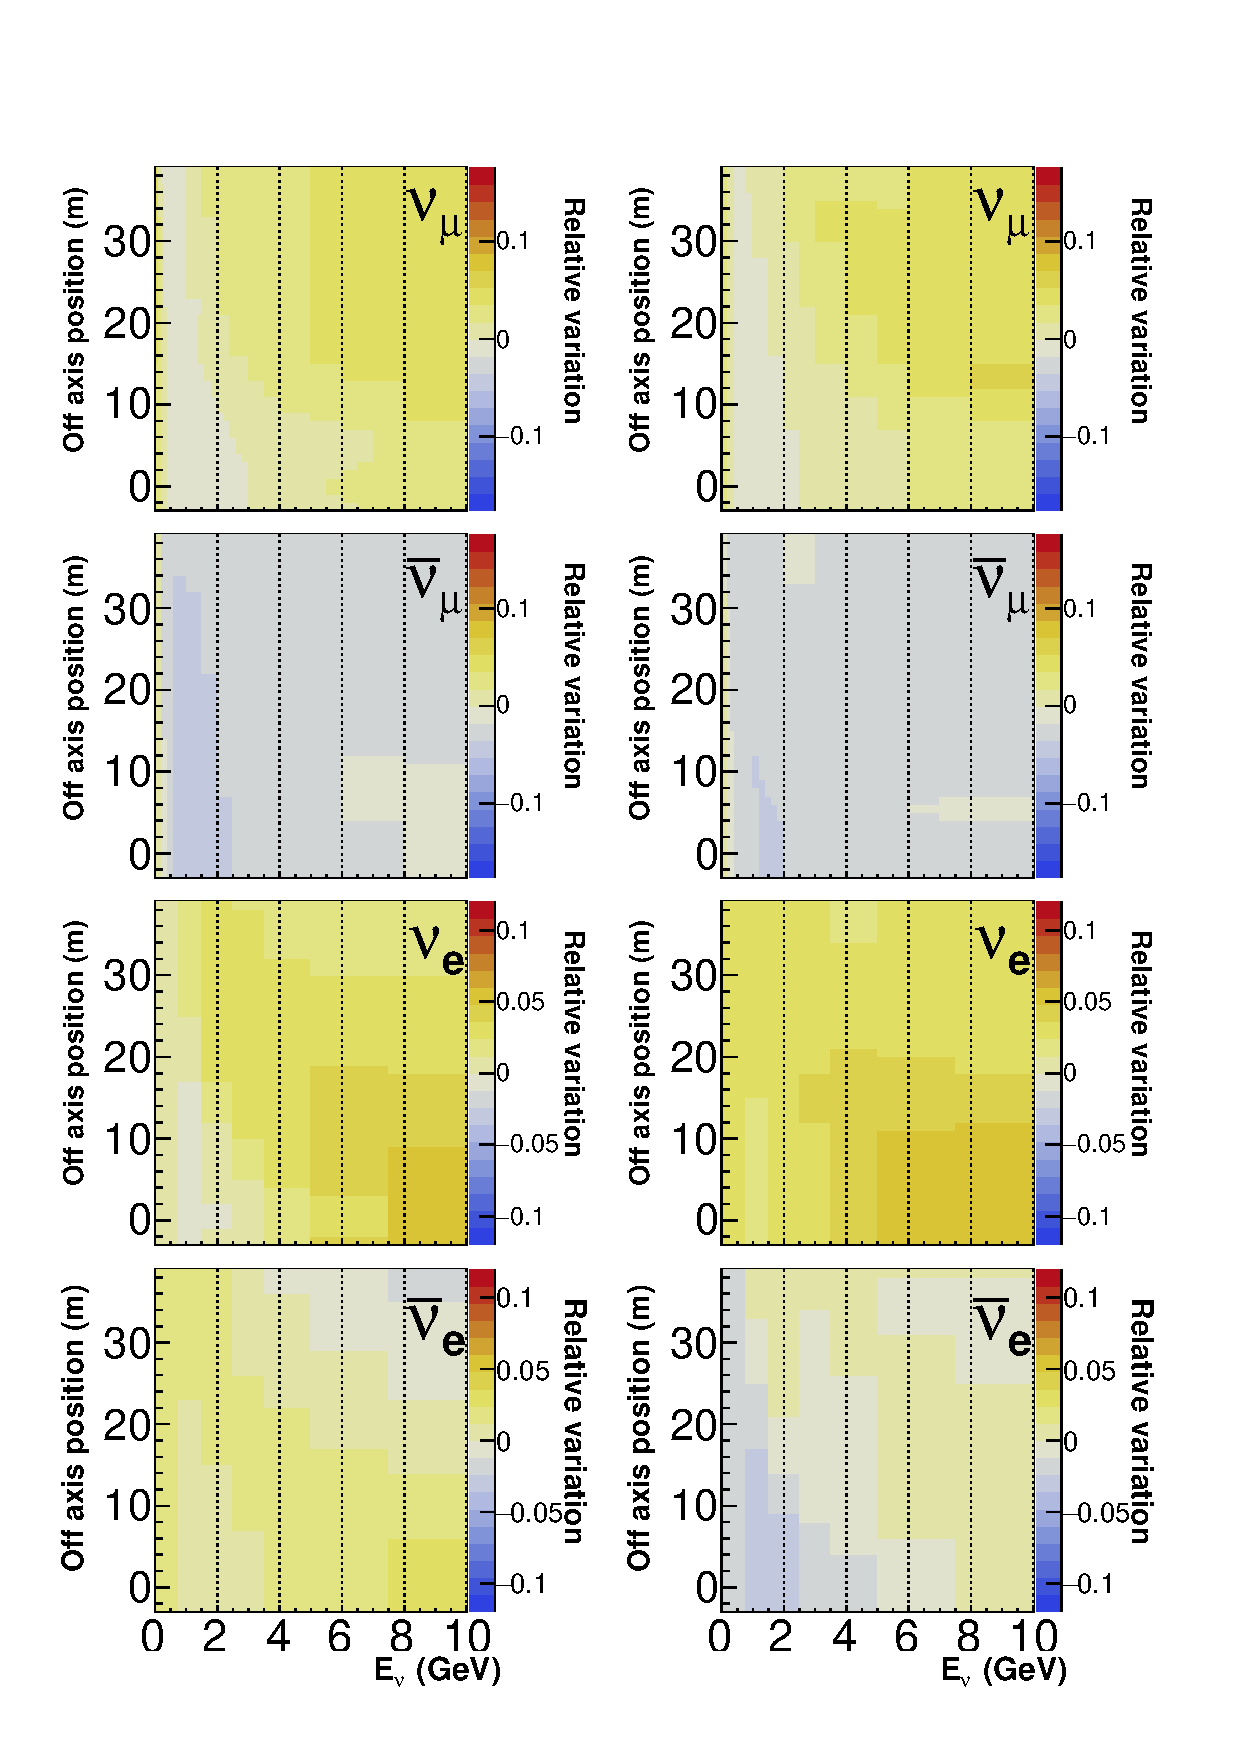
\includegraphics[width=0.95\textwidth]{plots/EvUncerts_offaxis_component_2_ppfxonly}
  \caption{The third most important eigen vector in the decomposition of the hadron production flux error matrix---including off axis near detector flux volumes---only the projection into the near detector flux predictions are shown. Here the flux predictions are averaged over the on axis flux volume. \textbf{N.B} This figure represents a recommended degree of freedom.}
  \label{fig:evfreedom_offaxis_c2_pppfxonly}
\end{figure}

\begin{figure}
  \centering
  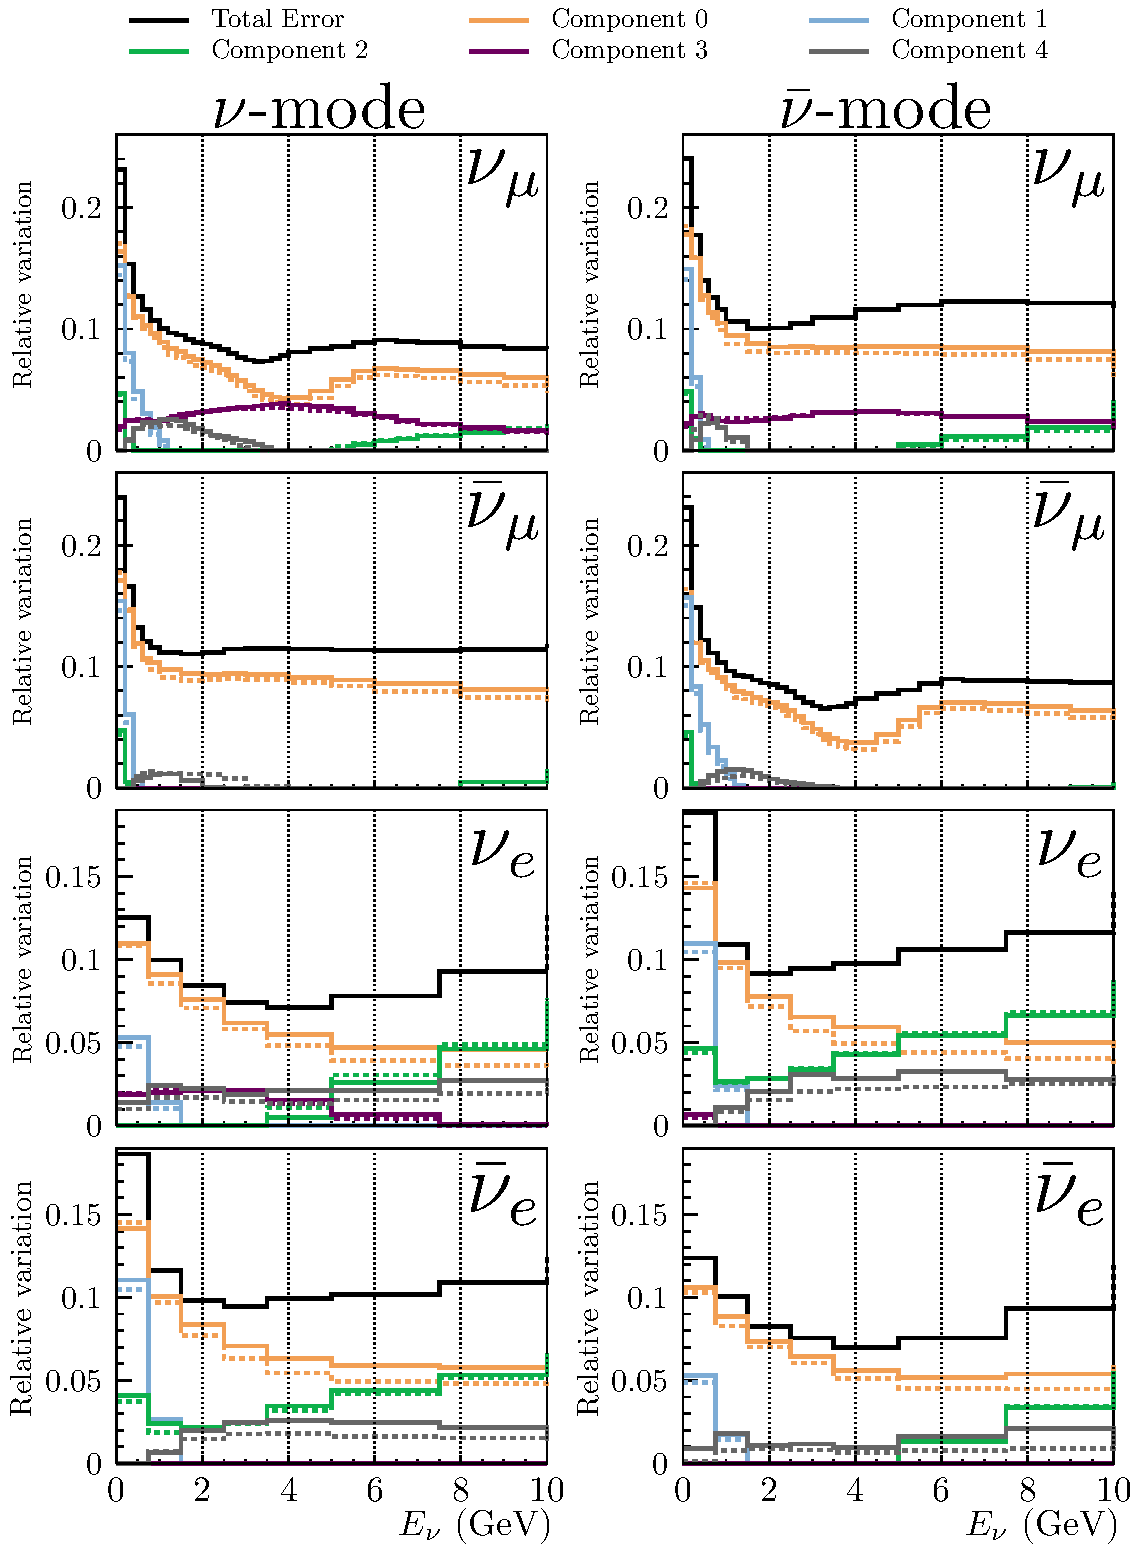
\includegraphics[width=0.95\textwidth]{plots/EvUncerts_allpca_ppfxcomp}
  \caption{The five most important eigen vectors in the decomposition of the on axis only total (solid) and hadron production (dashed) flux error matrices---only the projection into the near detector flux predictions are shown. Here the flux predictions are averaged over the on axis flux volume. \textbf{N.B.} The Total error prediction contains all degrees of freedom for both solid and dashed series. It can be seen that the total error is not affected by the choice of which degrees of freedom to include in the decomposition---as long as missing degrees of freedom are included in any error propagation separately.}
  \label{fig:evfreedom_onaxis_pppfxcomp}
\end{figure}


Finally, it is worth checking that including the off axis positions in the eigen-decomposition does not change the on-axis error substantially. The off axis positions correspond to an increase in the number of bins in the analysis from 378 to 4926, and it might be expected that the matrix decomposition might be affected. Fig.~\ref{fig:evfreedom_onaxis_oacomp} shows the most important five eigen vectors for the on axis\footnote{For ease of comparison these errors only cover the on-axis to 1m off axis window, whereas others in this section average over the 4 m on axis flux volume as described earlier.} position with (dashed) and without (solid) the off axis positions included. While the effect of individual components does change when including the off axis positions, the total error remains the same. Such variations may be expected as some systematic variations, notably variations in the focussing and alignment will become more important as off axis positions are included. As long as a large enough number of eigen vectors are included in any neutrino analysis, these differences should not affect the results.

\begin{figure}
  \centering
  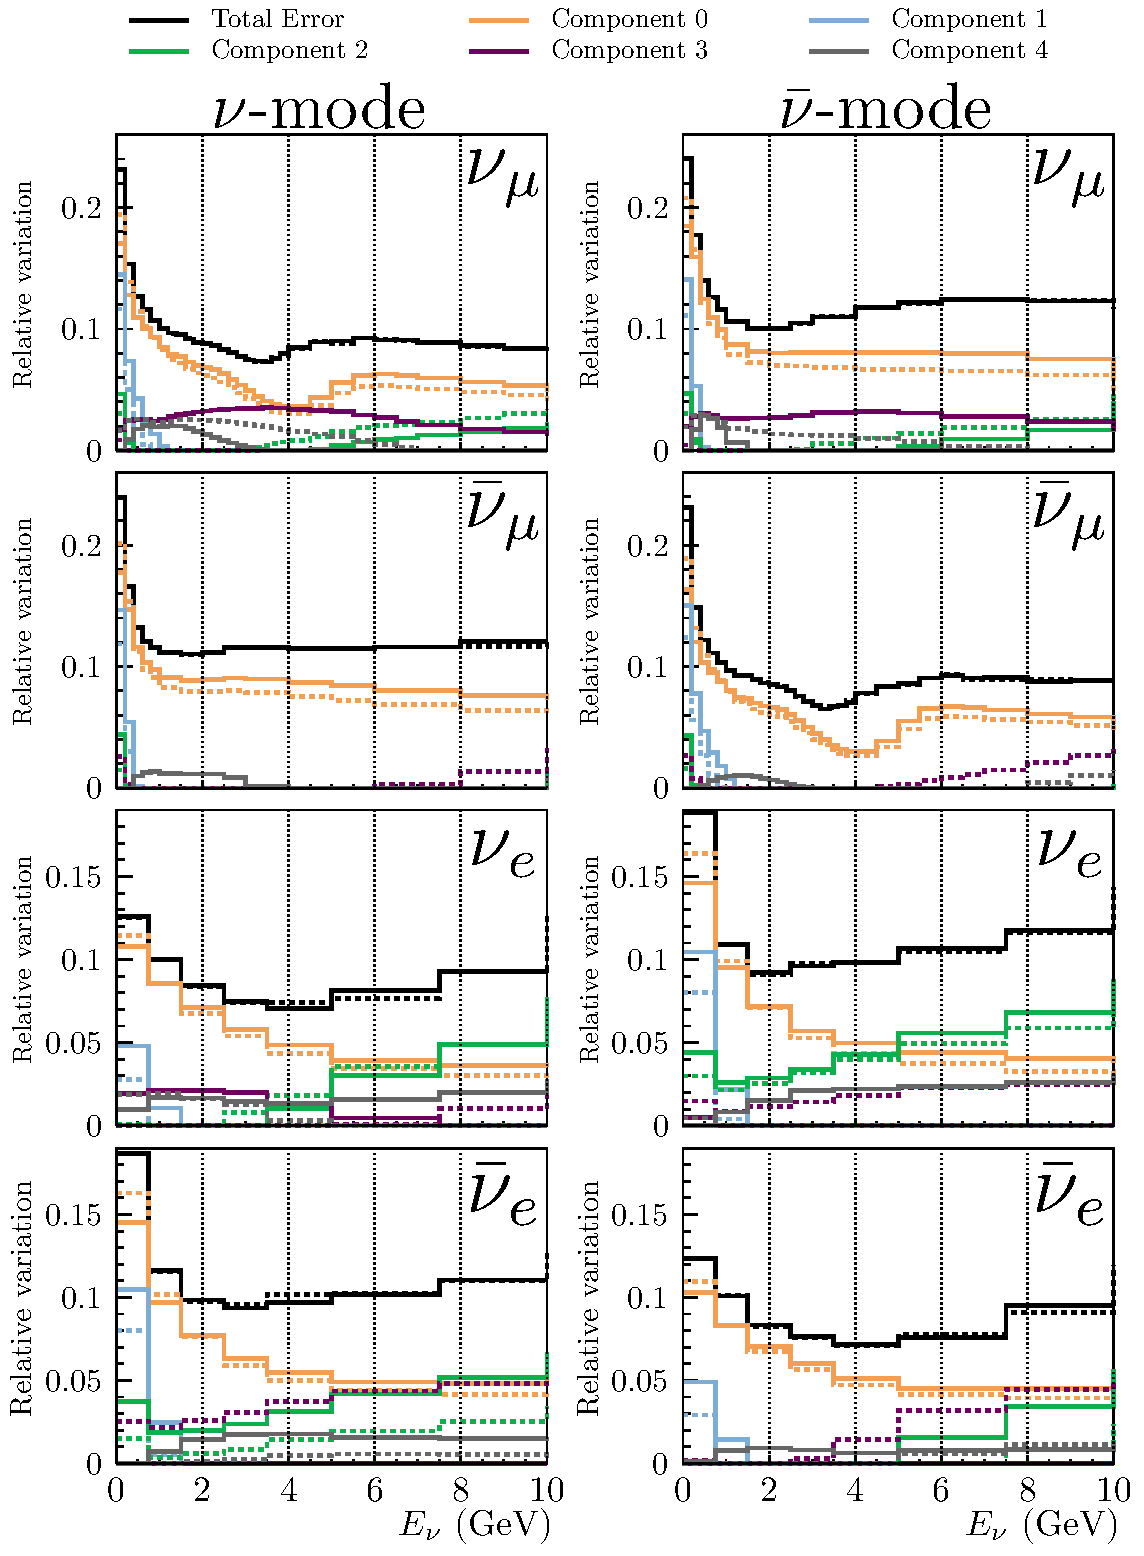
\includegraphics[width=0.95\textwidth]{plots/EvUncerts_oacomp}
  \caption{The five most important eigen vectors in the decomposition of the on axis only (solid) and off axis (dashed) hadron production flux error matrices---only the projection into the near detector flux predictions are shown. Here the flux predictions are averaged over a single 1 m wide slice at the on axis position. It can be seen that including the off axis positions does change the effect of a given component, this is not unexpected as some systematic variations onyl have significant effects off axis and thus will become more 'important' in the decompositon when off axis positions are included. The small changes in the total error at the on axis position may be due to the increased statistical noise when including the off axis positions, which increases the number of bins by an order of magnitude.}
  \label{fig:evfreedom_onaxis_oacomp}
\end{figure}

\section{Results}

The following subsections present the bin-by-bin fractional uncertainties for each beam mode and neutrino species for the near on axis, near off axis, and far detector flux volumes. For each, the error on the ratio of the near on axis and far detector prediction is also shown, as oscillation analyses generally make use of such systematic cancellation between the near and far detector.

It should be noted that all plots shown in this section were produced using the eigen-decompositions of the relevant component error matricies.

\subsection{Hadron production}

Systematic variations are calculated relative to the PPFX 'CV' tune, the relative variations should be applicable for DUNE, but it isn't clear that the CV tune itself is. 
When running PPFX, very large systematic universe weights were seen, for this analysis they were capped at 10. This restriction could be re-assessed in the future.

\begin{figure}
  \centering
  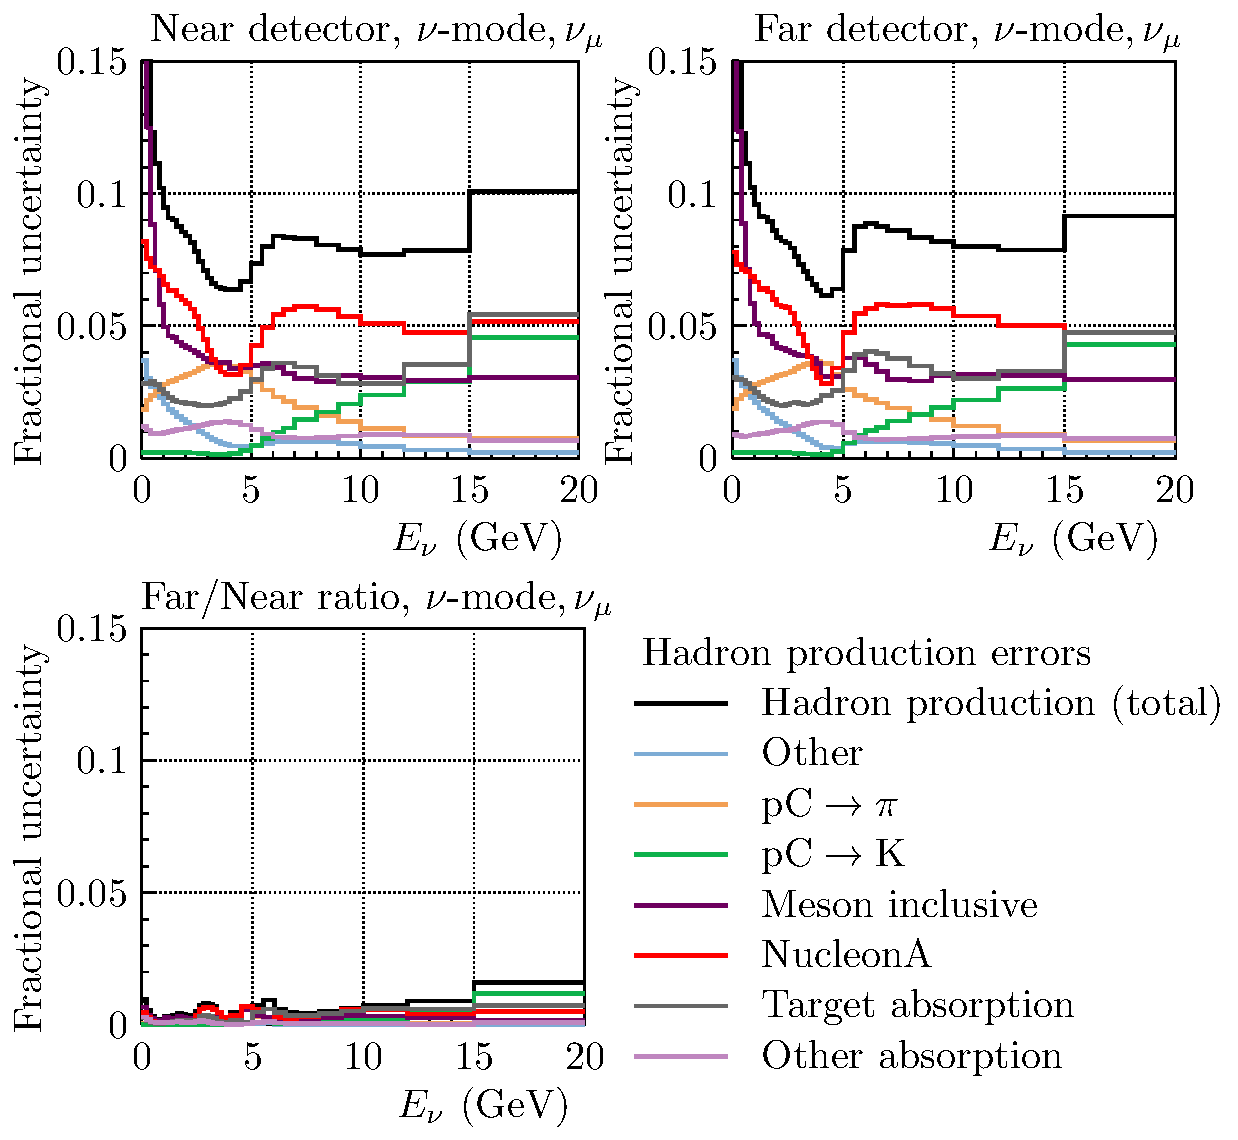
\includegraphics[width=0.7\textwidth]{plots/fracerrs/numode_numu_PPFX}
  \caption{The fractional uncertainty due to systematic variations in the hadron production model, the predicted uncertainty on the near prediction, far prediction, and the near/far ratio is shown for muon neutrinos in a neutrino-mode beam. Significant near-to-far cancellation is observed, from a error of ~8\% in the beam peak (2.3 GeV) for both near and far absolute rates, but the error on the near/far ratio can be seen to be less than a percent. The total uncertainty is broken down into some relevant categories of interactions in the beam target.}
  \label{fig:ppfx_nu_numu}
\end{figure}

\subsection{Focussing}

This section is somewhat poorly mis-named.

\begin{figure}
  \centering
  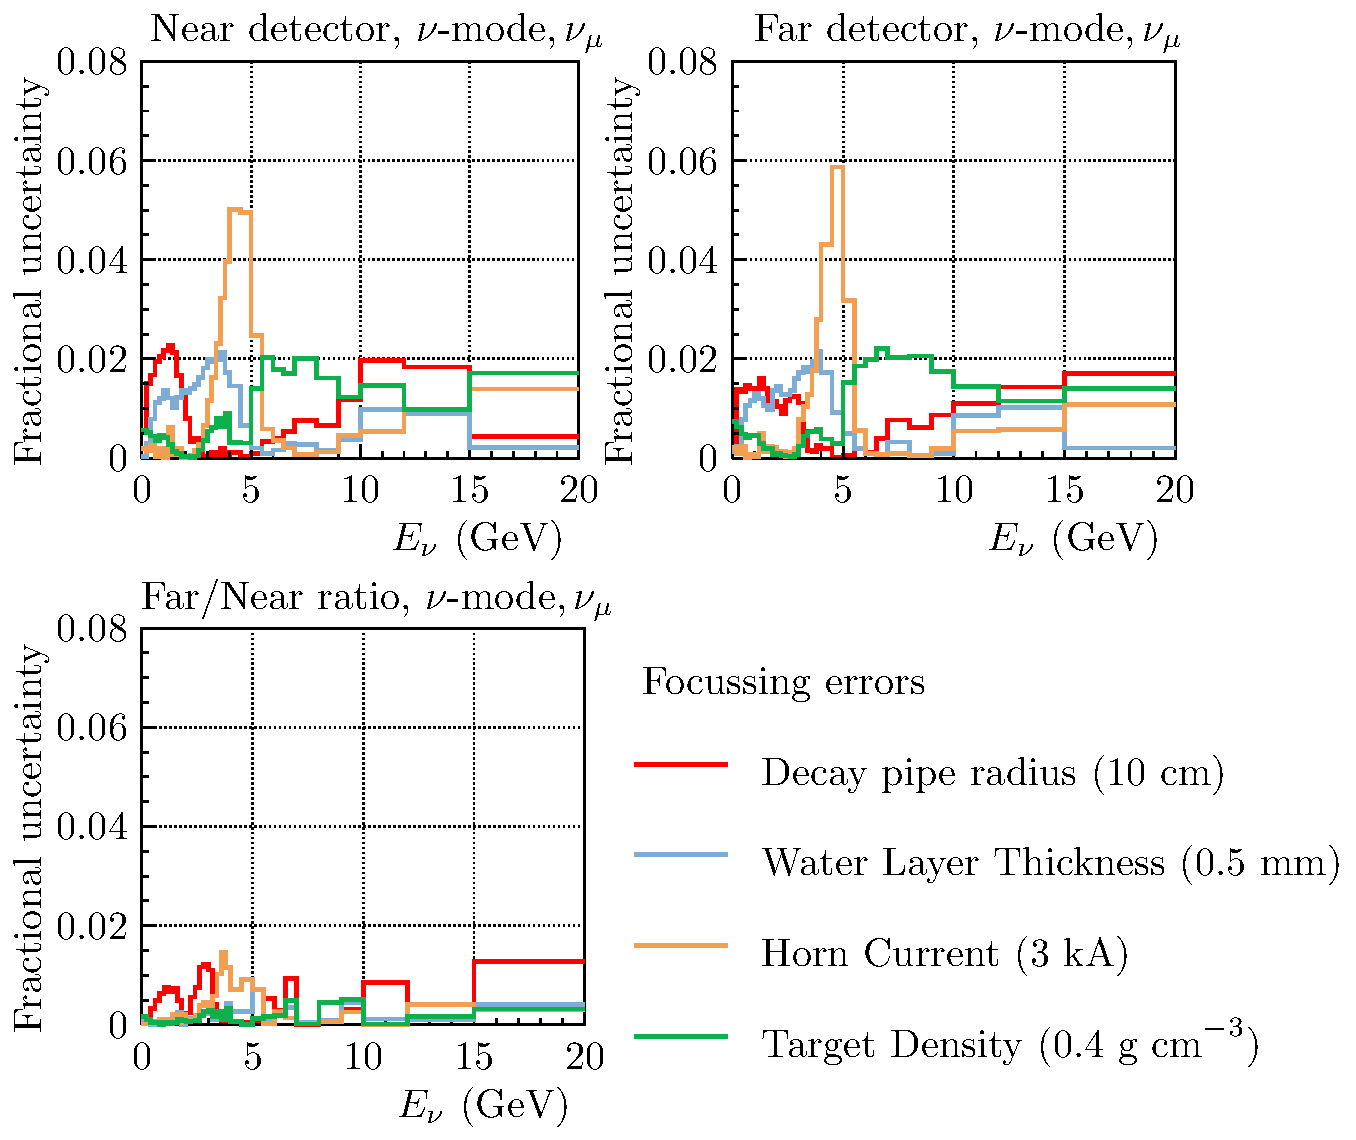
\includegraphics[width=0.7\textwidth]{plots/fracerrs/numode_numu_Focussing}
  \caption{The fractional uncertainty due to systematic variations in 'focussing' elements of the beam line, the predicted uncertainty on the near prediction, far prediction, and the near/far ratio is shown for muon neutrinos in a neutrino-mode beam. }
  \label{fig:foc_nu_numu}
\end{figure}

\begin{figure}
  \centering
  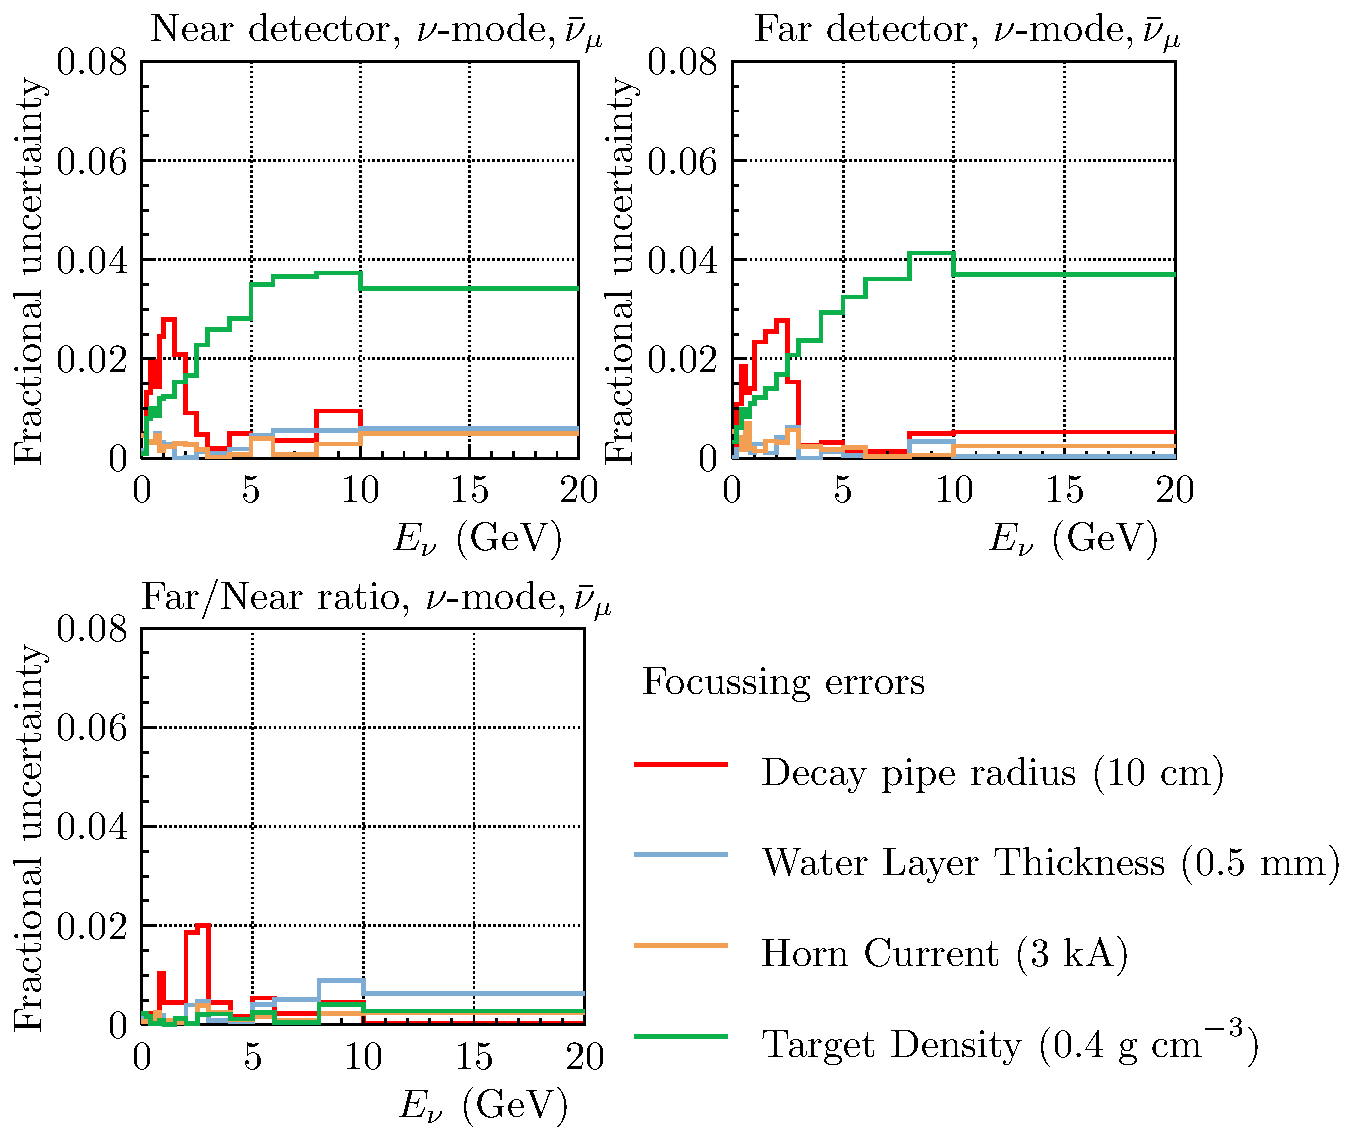
\includegraphics[width=0.7\textwidth]{plots/fracerrs/numode_numubar_Focussing}
  \caption{The fractional uncertainty due to systematic variations in 'focussing' elements of the beam line, the predicted uncertainty on the near prediction, far prediction, and the near/far ratio is shown for muon antineutrinos in a neutrino-mode beam.}
  \label{fig:foc_nu_numubar}
\end{figure}

\begin{figure}
  \centering
  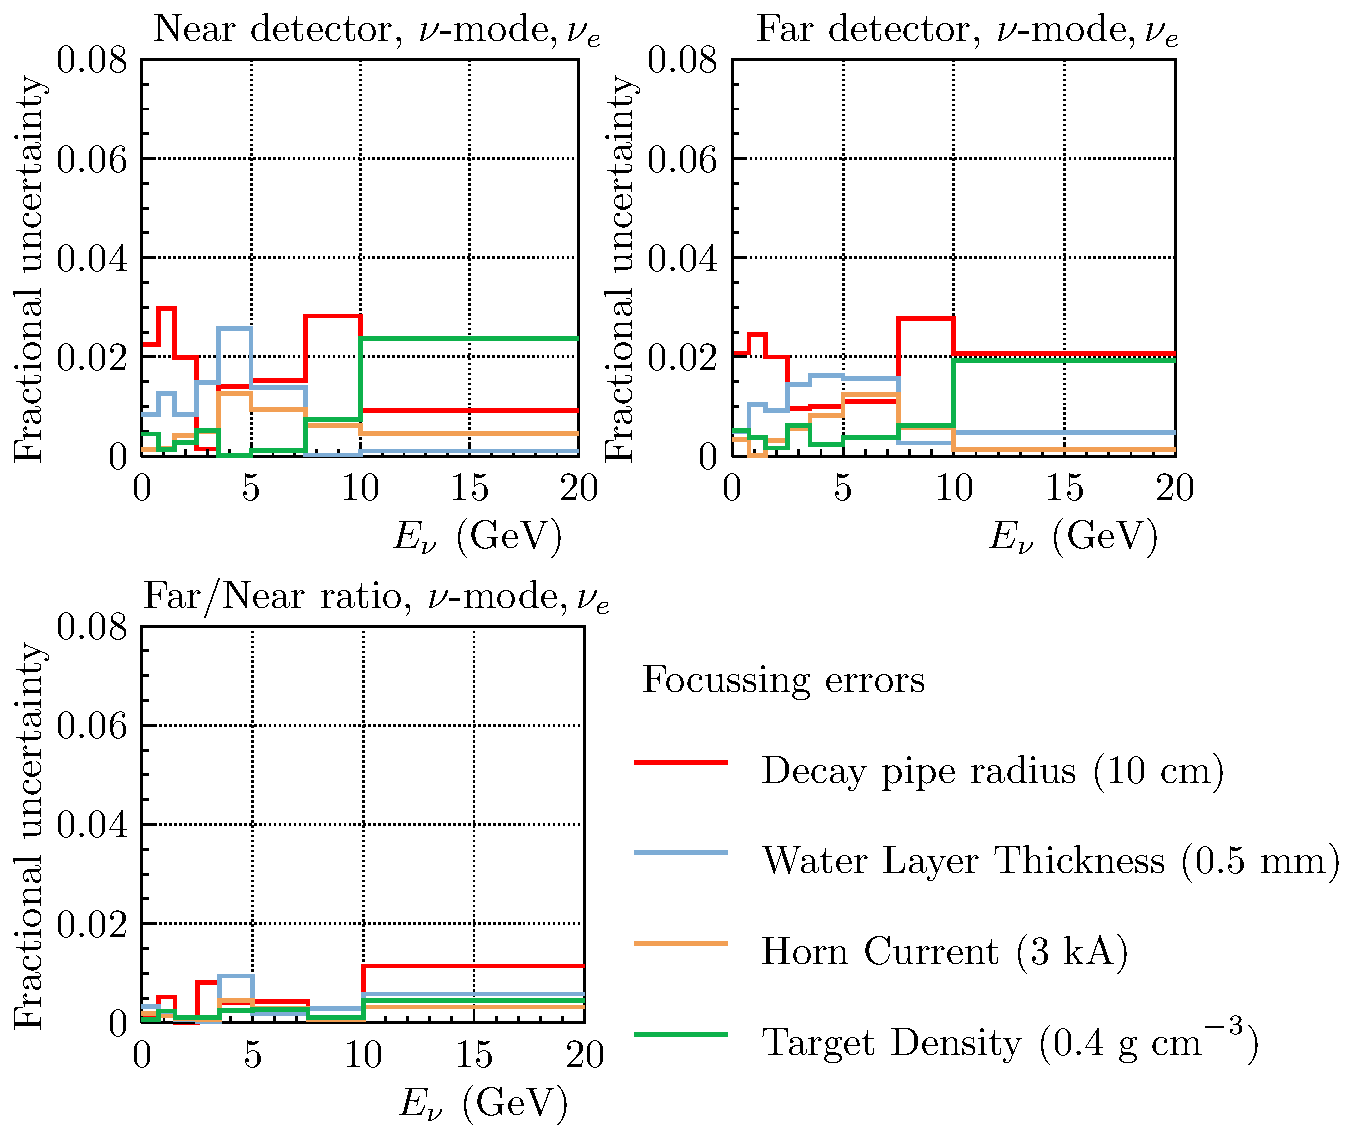
\includegraphics[width=0.7\textwidth]{plots/fracerrs/numode_nue_Focussing}
  \caption{The fractional uncertainty due to systematic variations in 'focussing' elements of the beam line, the predicted uncertainty on the near prediction, far prediction, and the near/far ratio is shown for electron neutrinos in a neutrino-mode beam.}
  \label{fig:foc_nu_nue}
\end{figure}

\begin{figure}
  \centering
  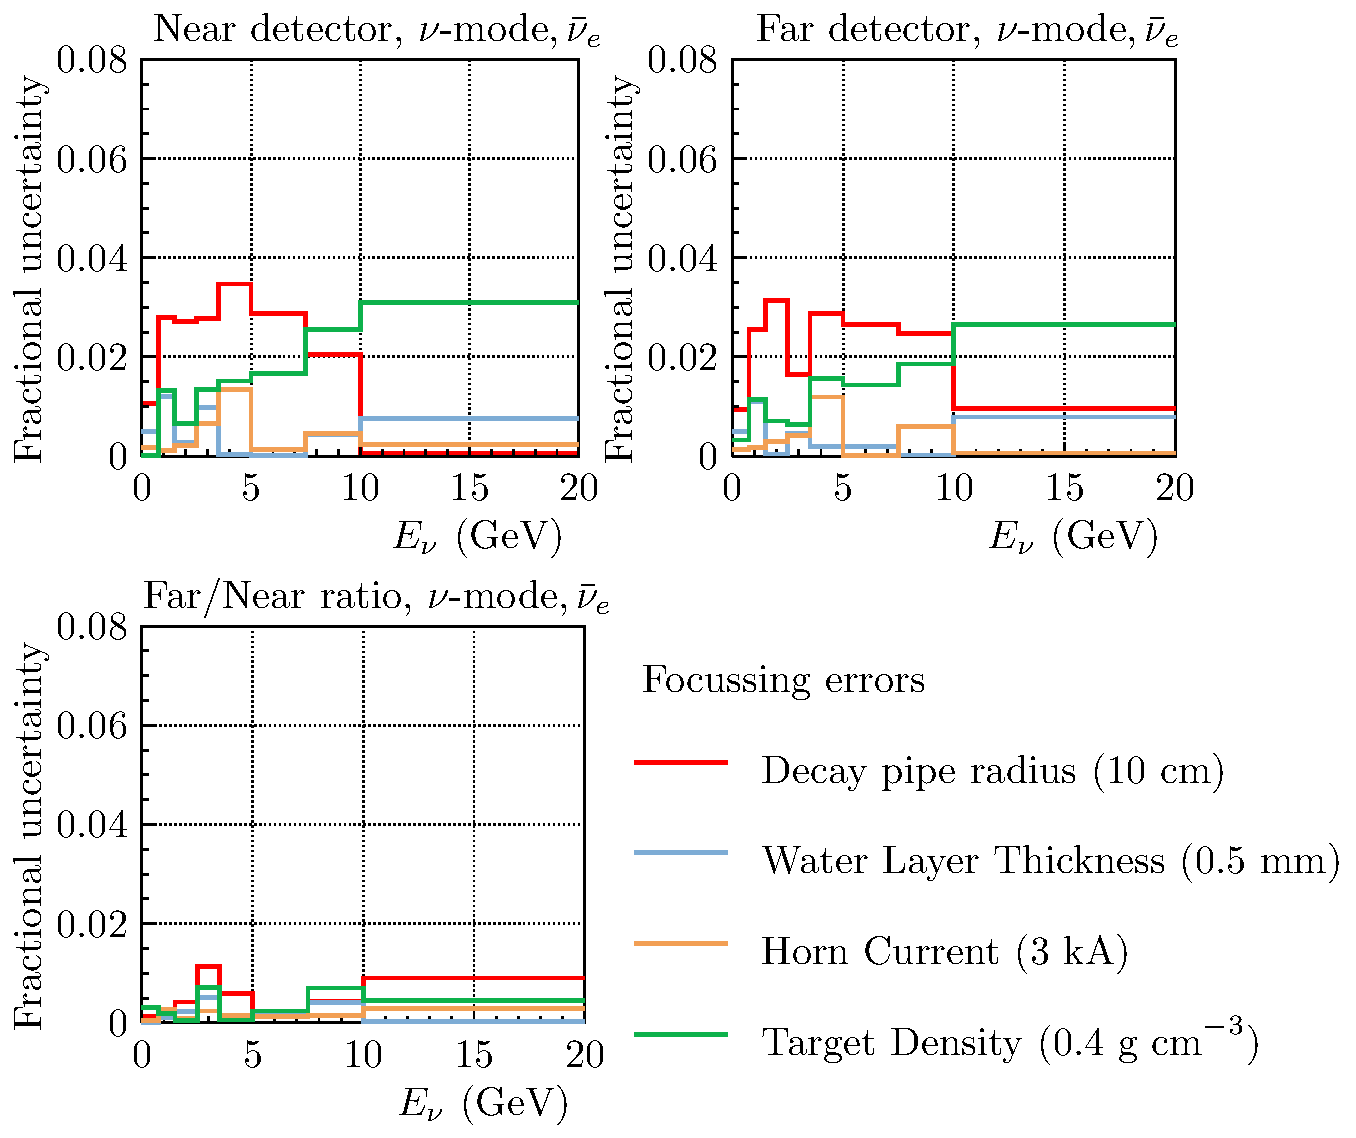
\includegraphics[width=0.7\textwidth]{plots/fracerrs/numode_nuebar_Focussing}
  \caption{The fractional uncertainty due to systematic variations in 'focussing' elements of the beam line, the predicted uncertainty on the near prediction, far prediction, and the near/far ratio is shown for electron antineutrinos in a neutrino-mode beam.}
  \label{fig:foc_nu_nuebar}
\end{figure}

\begin{figure}
  \centering
  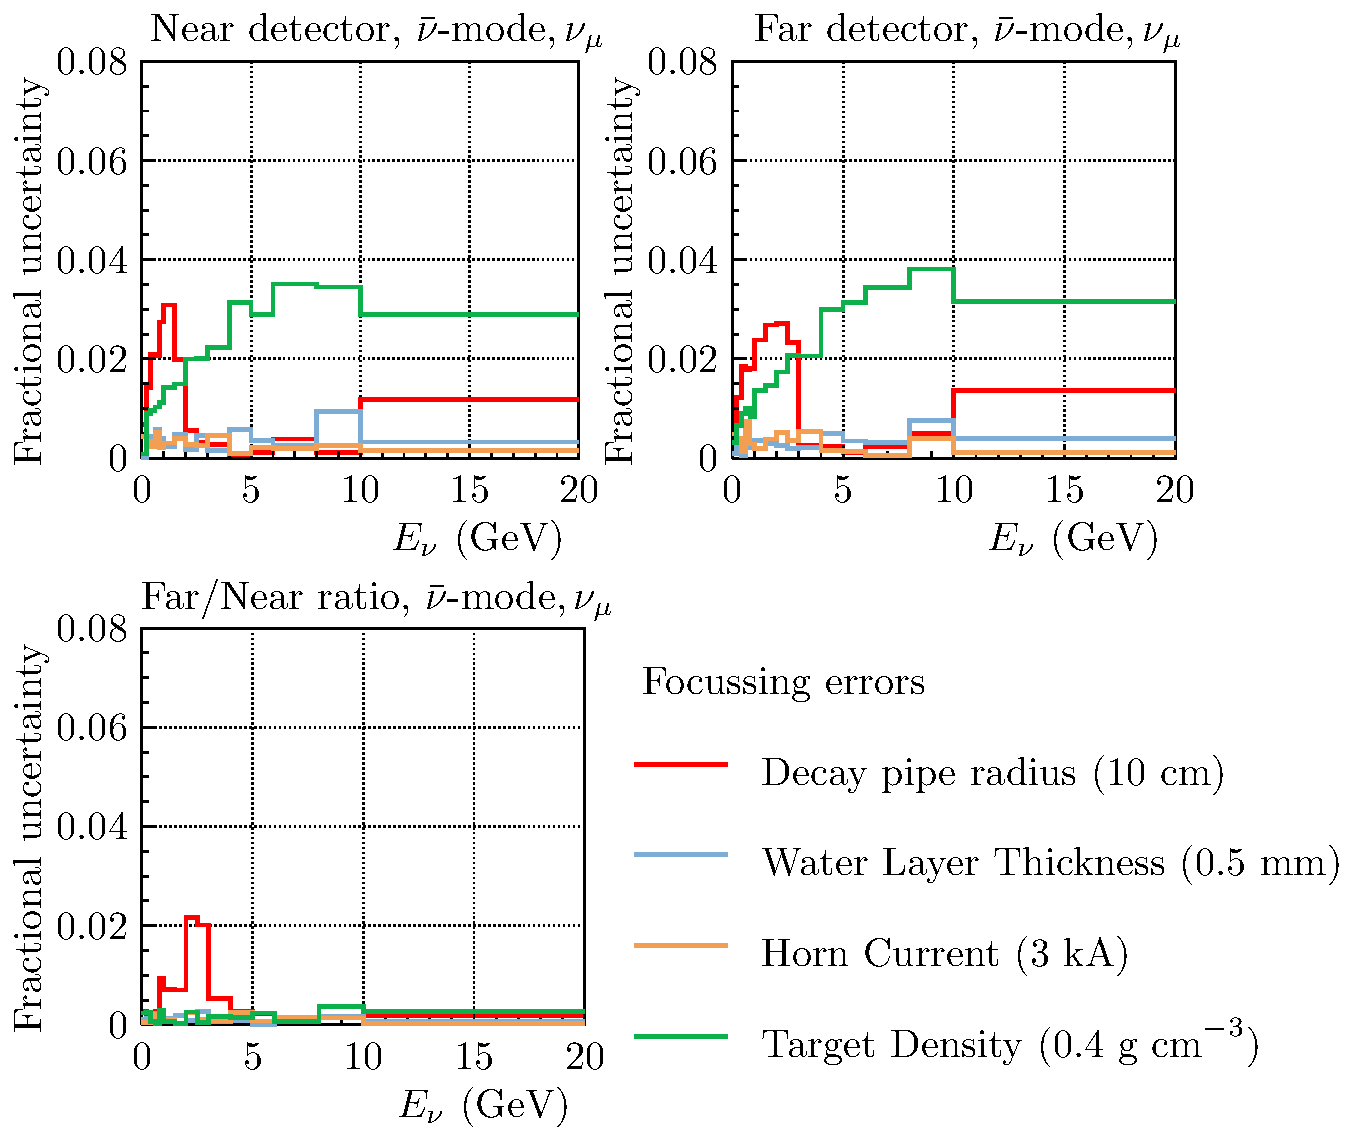
\includegraphics[width=0.7\textwidth]{plots/fracerrs/nubarmode_numu_Focussing}
  \caption{The fractional uncertainty due to systematic variations in 'focussing' elements of the beam line, the predicted uncertainty on the near prediction, far prediction, and the near/far ratio is shown for muon neutrinos in a antineutrino-mode beam.}
  \label{fig:foc_nubar_numu}
\end{figure}

\begin{figure}
  \centering
  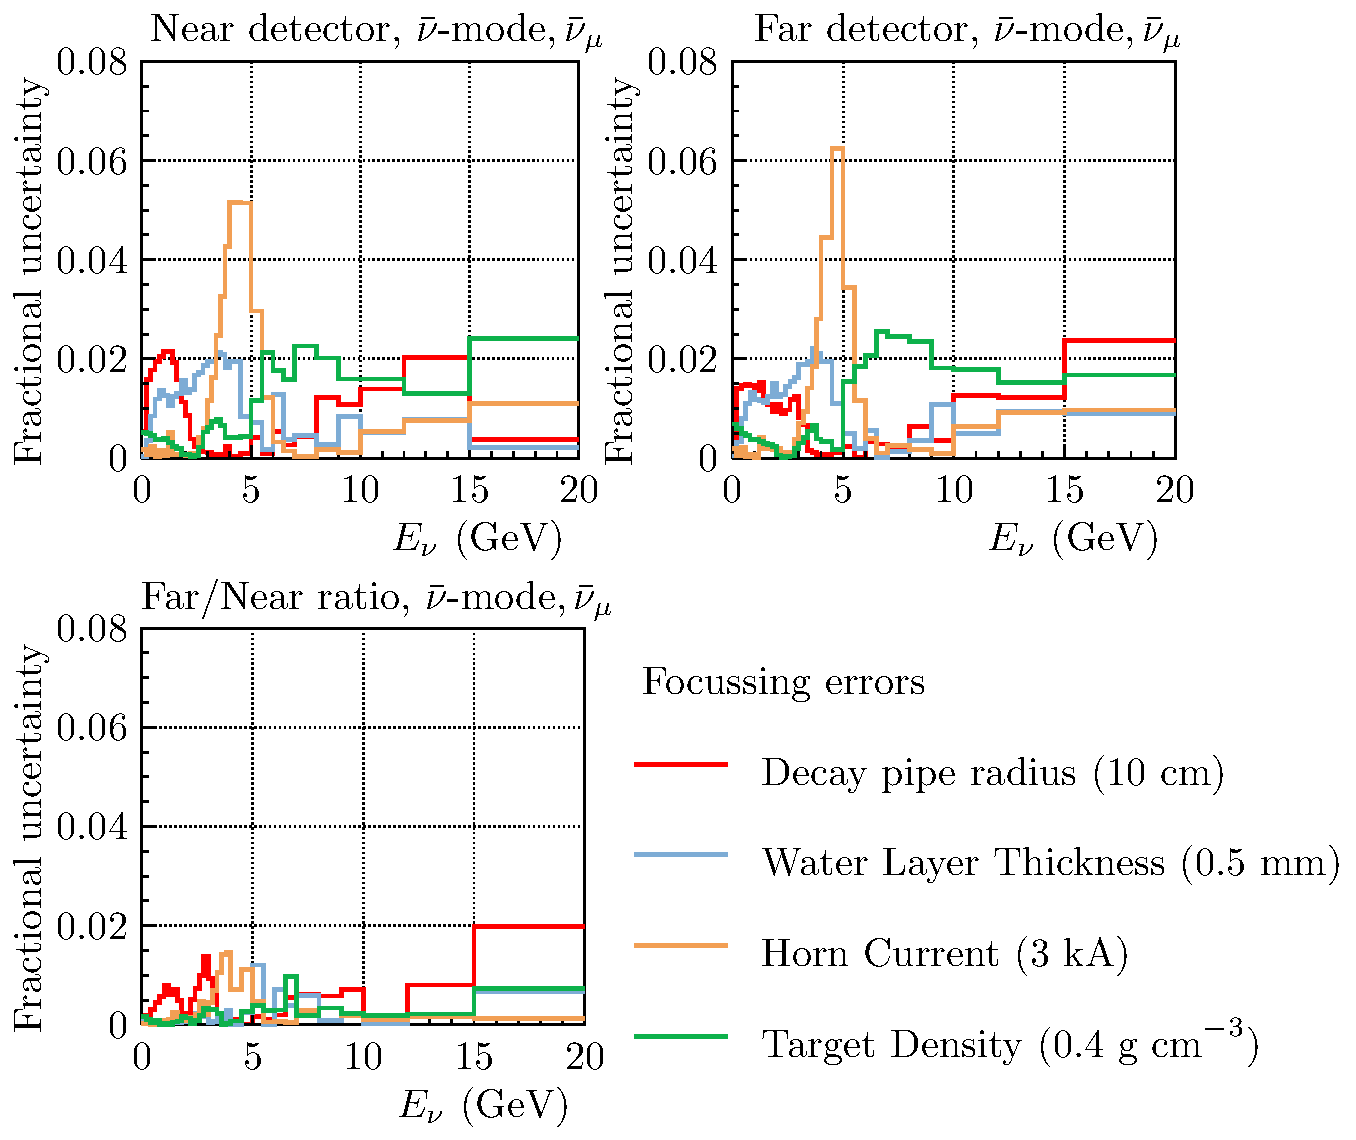
\includegraphics[width=0.7\textwidth]{plots/fracerrs/nubarmode_numubar_Focussing}
  \caption{The fractional uncertainty due to systematic variations in 'focussing' elements of the beam line, the predicted uncertainty on the near prediction, far prediction, and the near/far ratio is shown for muon antineutrinos in a antineutrino-mode beam.}
  \label{fig:foc_nubar_numubar}
\end{figure}

\begin{figure}
  \centering
  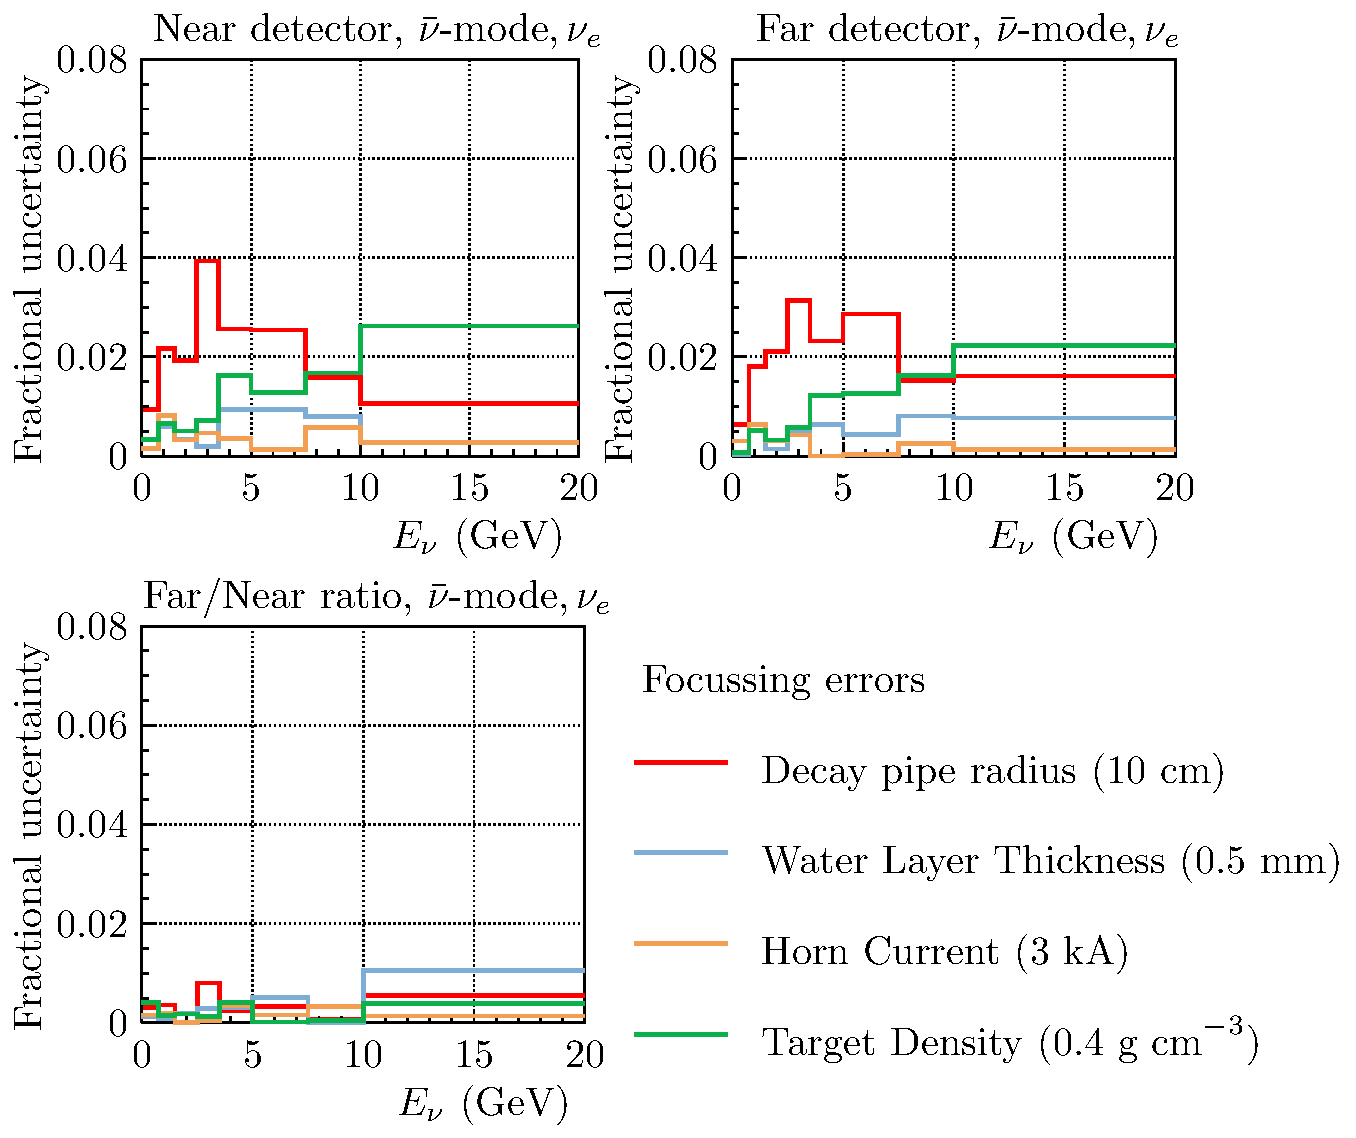
\includegraphics[width=0.7\textwidth]{plots/fracerrs/nubarmode_nue_Focussing}
  \caption{The fractional uncertainty due to systematic variations in 'focussing' elements of the beam line, the predicted uncertainty on the near prediction, far prediction, and the near/far ratio is shown for electron neutrinos in a antineutrino-mode beam.}
  \label{fig:foc_nubar_nue}
\end{figure}

\begin{figure}
  \centering
  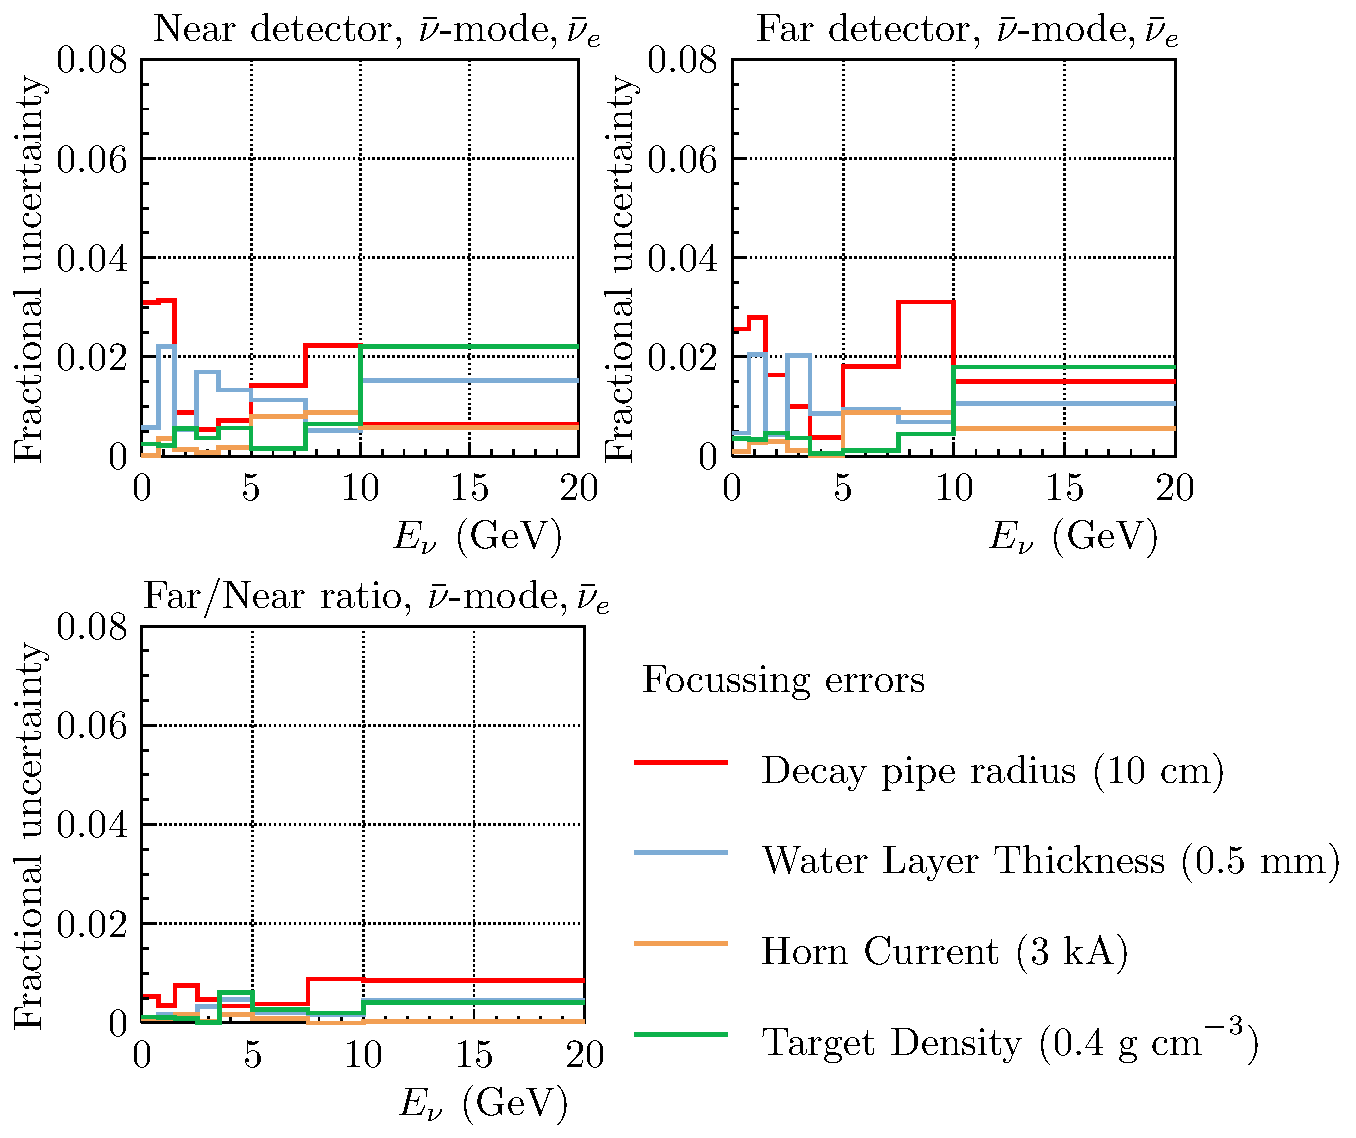
\includegraphics[width=0.7\textwidth]{plots/fracerrs/nubarmode_nuebar_Focussing}
  \caption{The fractional uncertainty due to systematic variations in 'focussing' elements of the beam line, the predicted uncertainty on the near prediction, far prediction, and the near/far ratio is shown for electron antineutrinos in a antineutrino-mode beam.}
  \label{fig:foc_nubar_nuebar}
\end{figure}

\subsection{Horn Alignment}


\begin{figure}
  \centering
  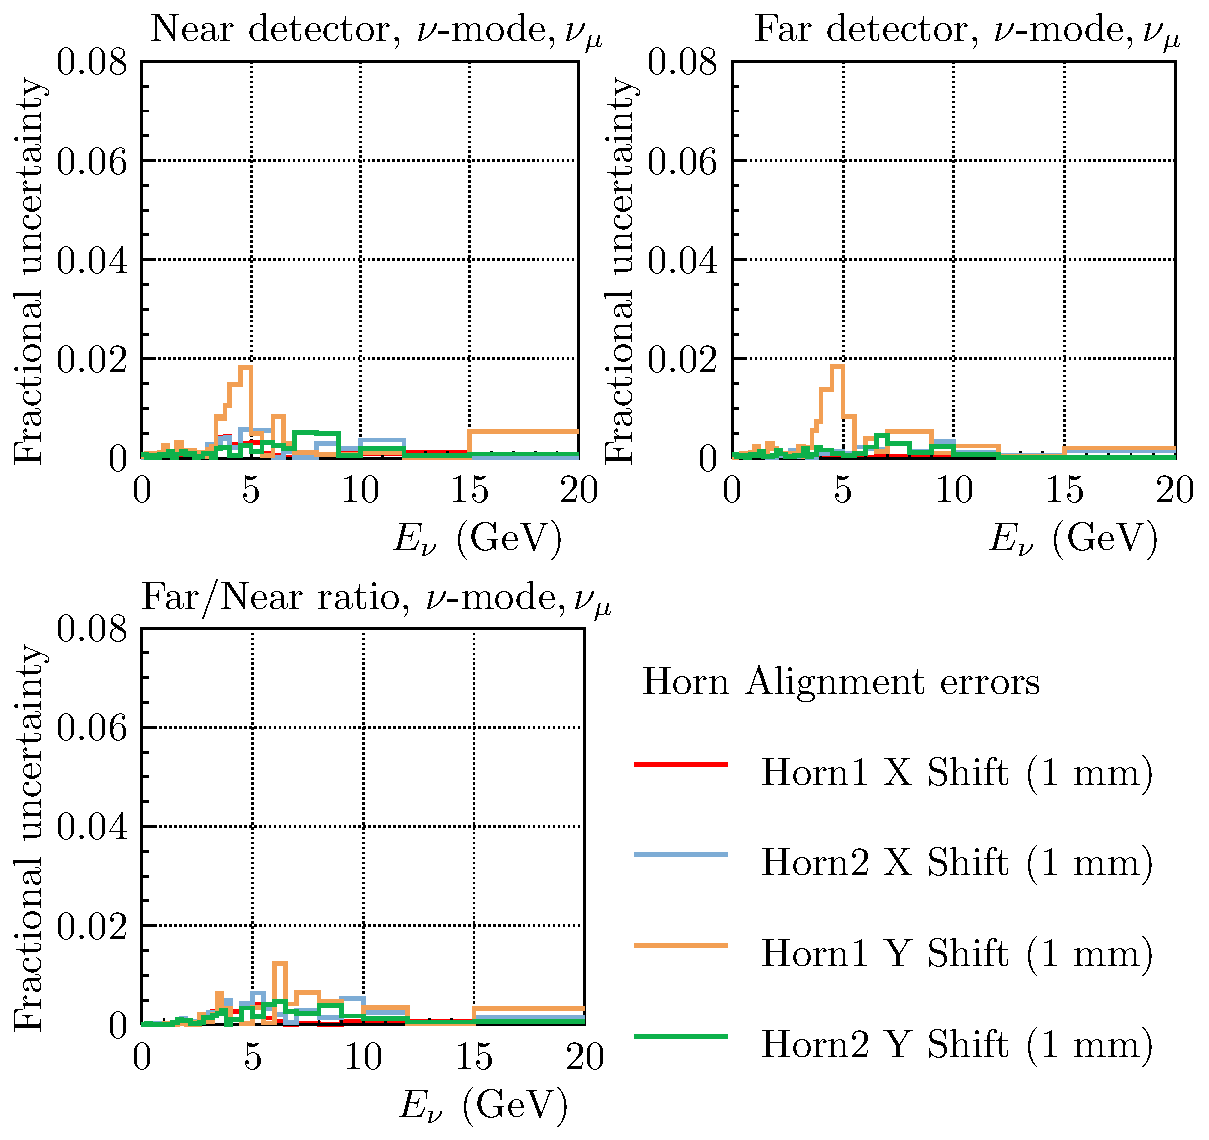
\includegraphics[width=0.65\textwidth]{plots/fracerrs/numode_numu_HornAlignment}
  \caption{The fractional uncertainty due to systematic variations in the alignment of the neutrino horns, the predicted uncertainty on the near prediction, far prediction, and the near/far ratio is shown for muon neutrinos in a neutrino-mode beam. }
  \label{fig:hornalign_nu_numu}
\end{figure}

\begin{figure}
  \centering
  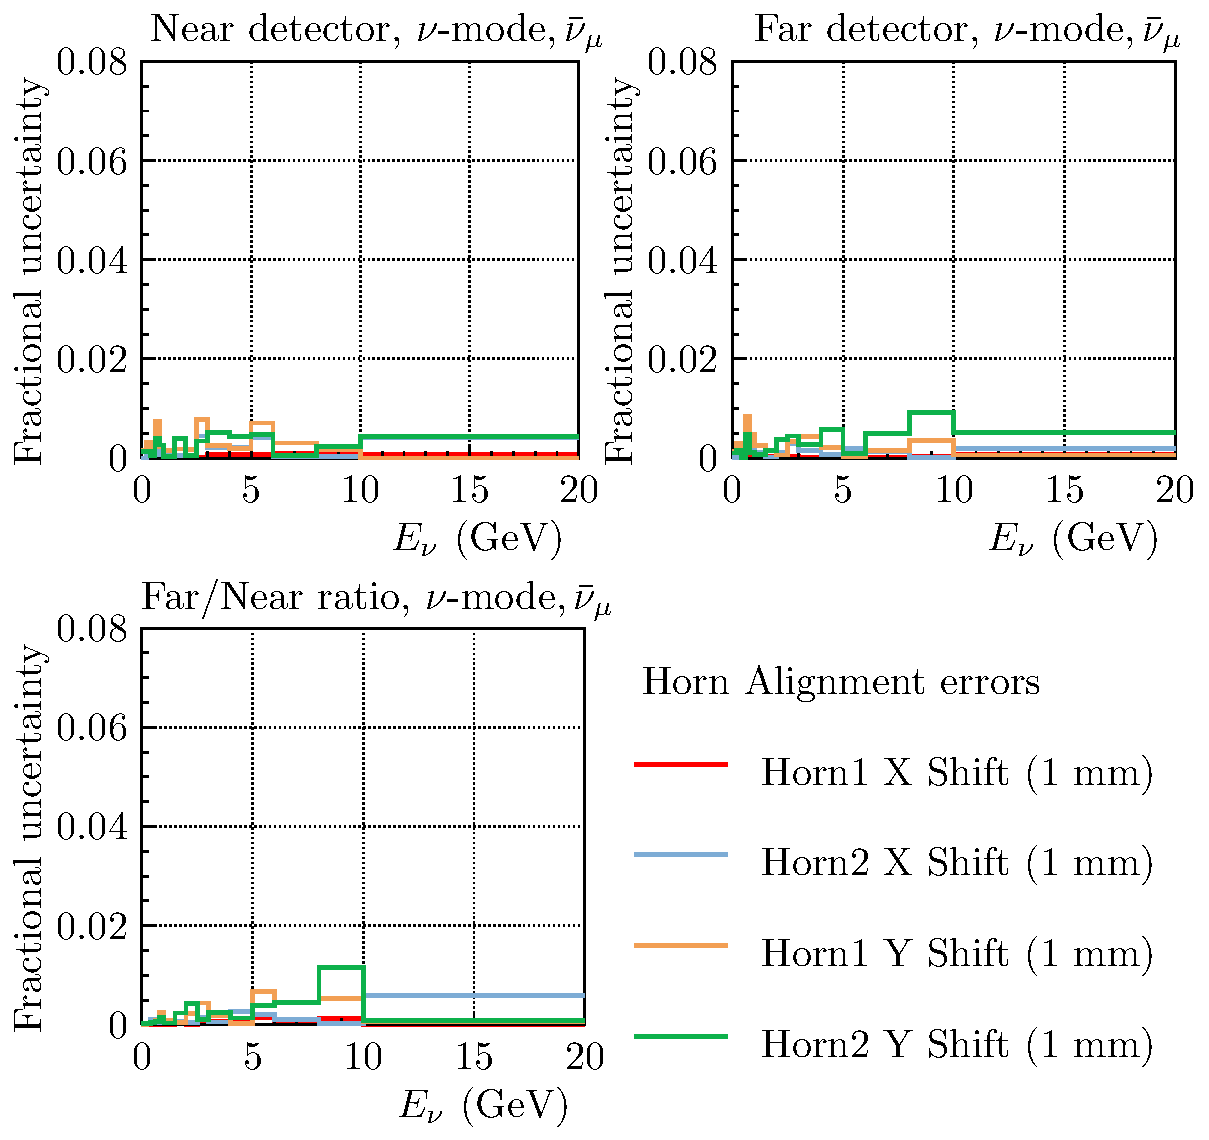
\includegraphics[width=0.65\textwidth]{plots/fracerrs/numode_numubar_HornAlignment}
  \caption{The fractional uncertainty due to systematic variations in the alignment of the neutrino horns, the predicted uncertainty on the near prediction, far prediction, and the near/far ratio is shown for muon antineutrinos in a neutrino-mode beam.}
  \label{fig:hornalign_nu_numubar}
\end{figure}

\begin{figure}
  \centering
  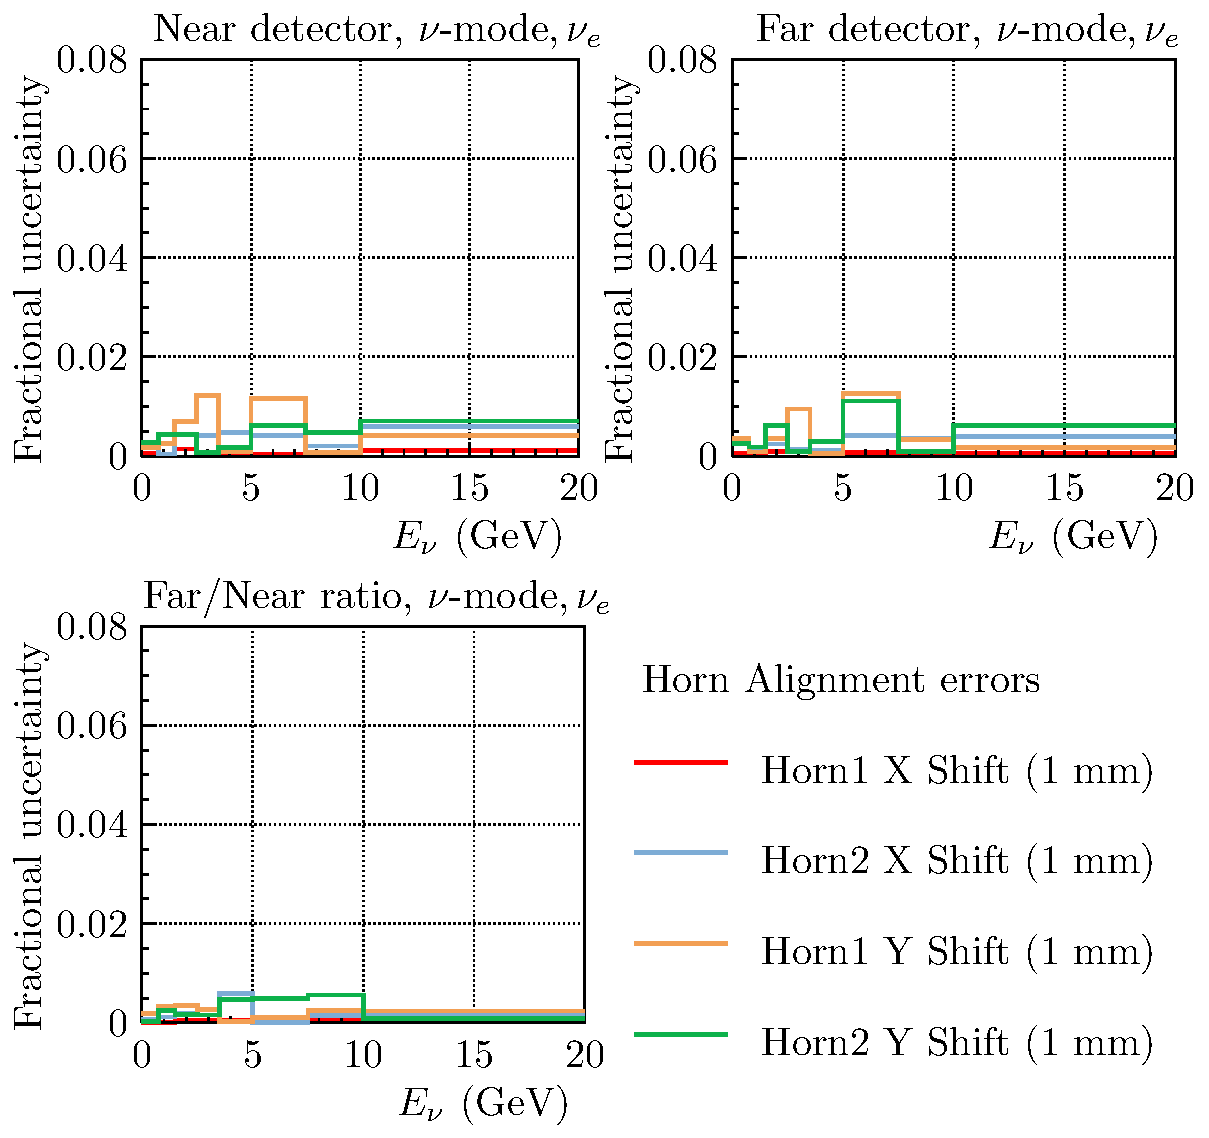
\includegraphics[width=0.65\textwidth]{plots/fracerrs/numode_nue_HornAlignment}
  \caption{The fractional uncertainty due to systematic variations in the alignment of the neutrino horns, the predicted uncertainty on the near prediction, far prediction, and the near/far ratio is shown for electron neutrinos in a neutrino-mode beam.}
  \label{fig:hornalign_nu_nue}
\end{figure}

\begin{figure}
  \centering
  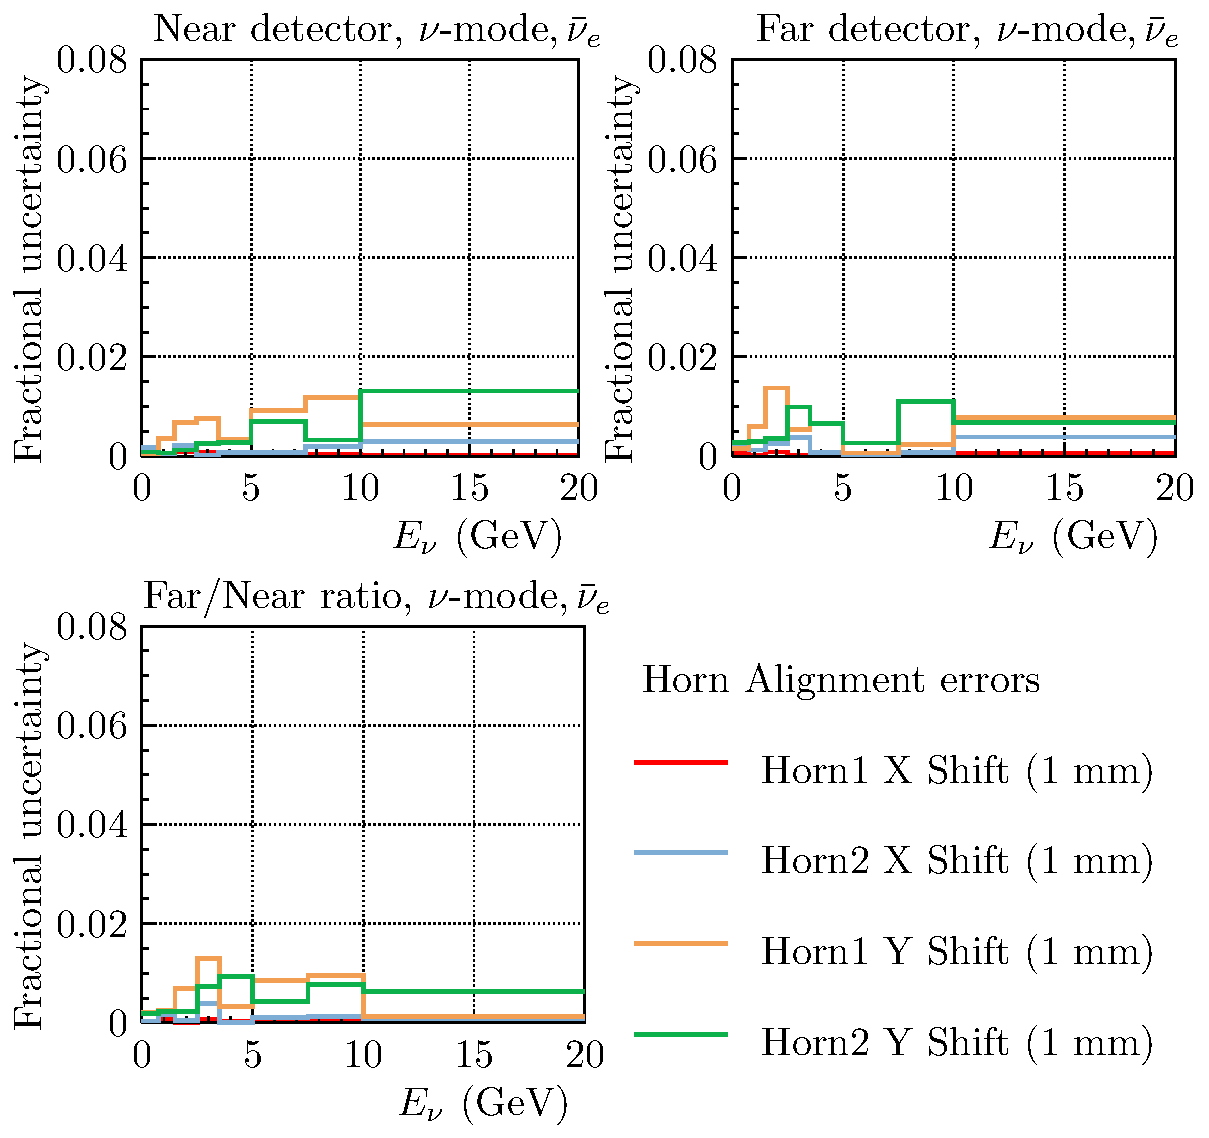
\includegraphics[width=0.65\textwidth]{plots/fracerrs/numode_nuebar_HornAlignment}
  \caption{The fractional uncertainty due to systematic variations in the alignment of the neutrino horns, the predicted uncertainty on the near prediction, far prediction, and the near/far ratio is shown for electron antineutrinos in a neutrino-mode beam.}
  \label{fig:hornalign_nu_nuebar}
\end{figure}

\begin{figure}
  \centering
  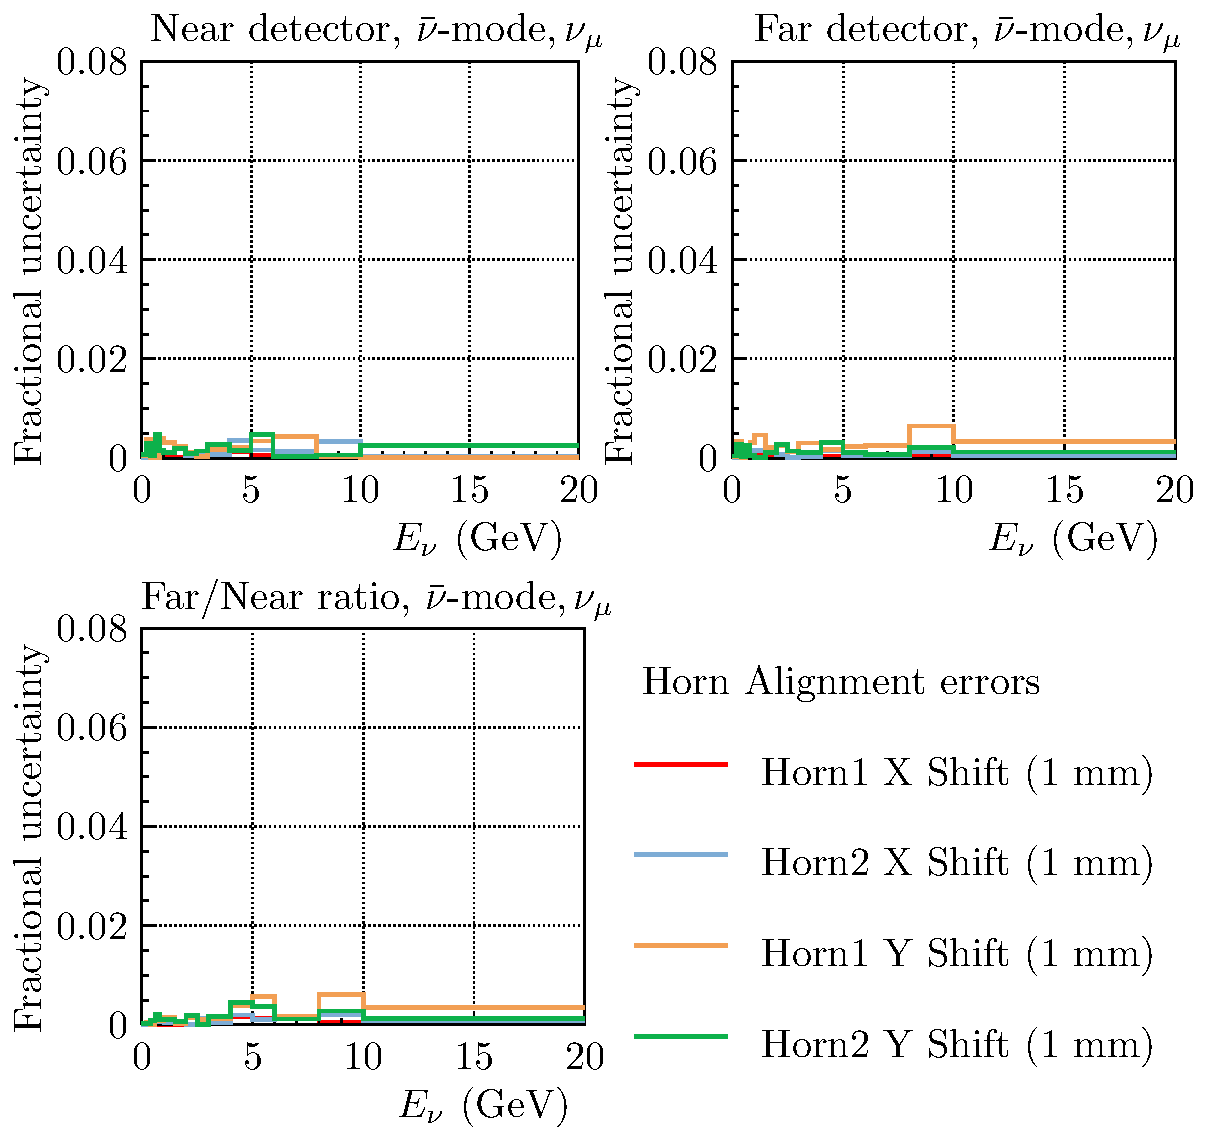
\includegraphics[width=0.65\textwidth]{plots/fracerrs/nubarmode_numu_HornAlignment}
  \caption{The fractional uncertainty due to systematic variations in the alignment of the neutrino horns, the predicted uncertainty on the near prediction, far prediction, and the near/far ratio is shown for muon neutrinos in a antineutrino-mode beam.}
  \label{fig:hornalign_nubar_numu}
\end{figure}

\begin{figure}
  \centering
  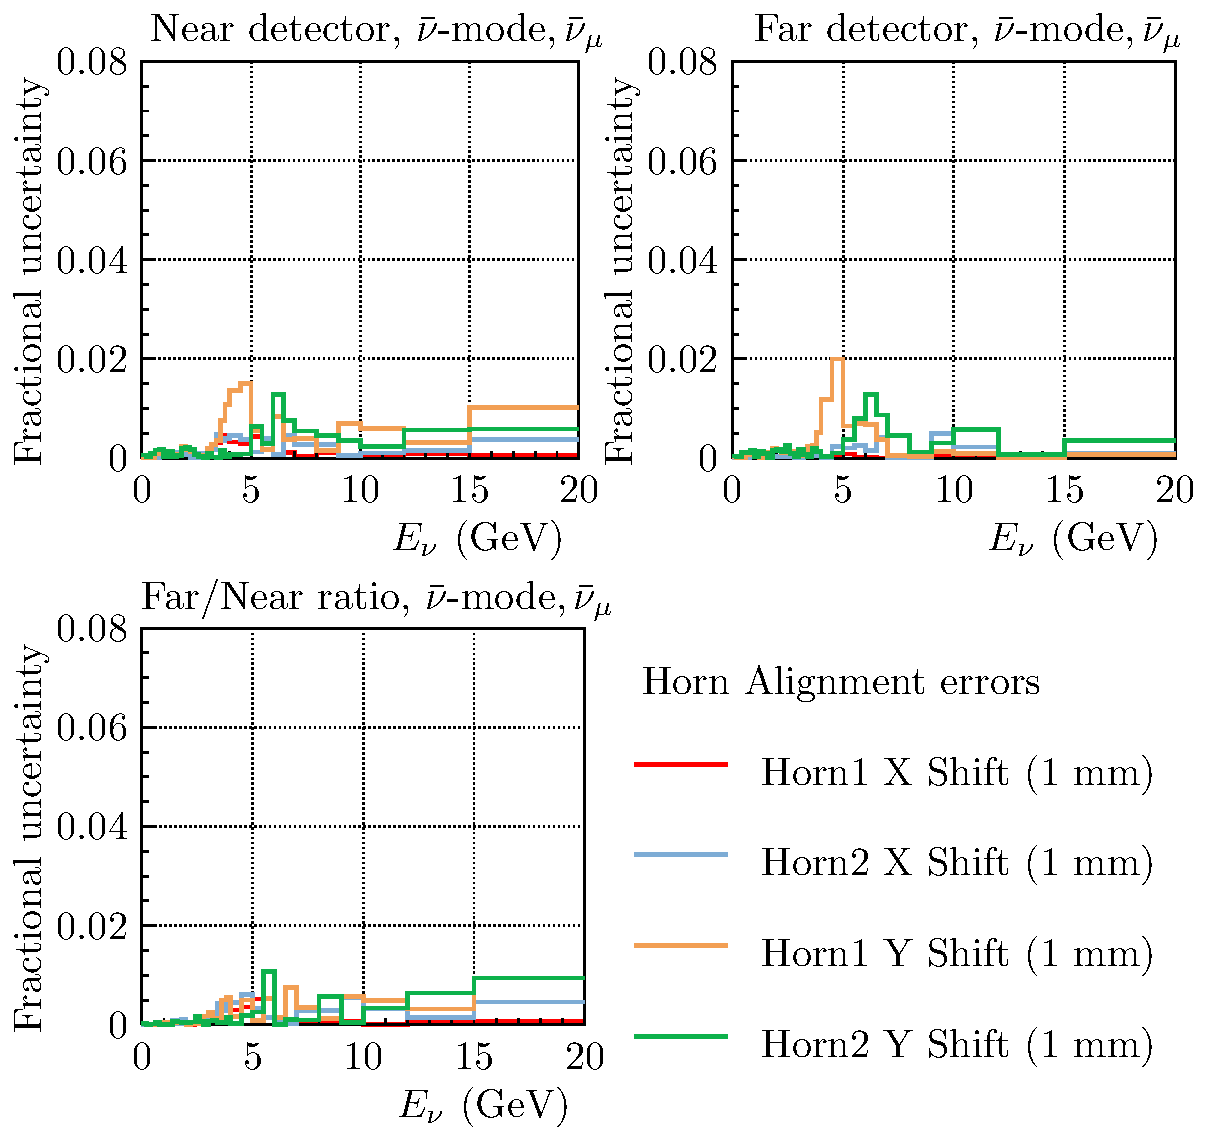
\includegraphics[width=0.65\textwidth]{plots/fracerrs/nubarmode_numubar_HornAlignment}
  \caption{The fractional uncertainty due to systematic variations in the alignment of the neutrino horns, the predicted uncertainty on the near prediction, far prediction, and the near/far ratio is shown for muon antineutrinos in a antineutrino-mode beam.}
  \label{fig:hornalign_nubar_numubar}
\end{figure}

\begin{figure}
  \centering
  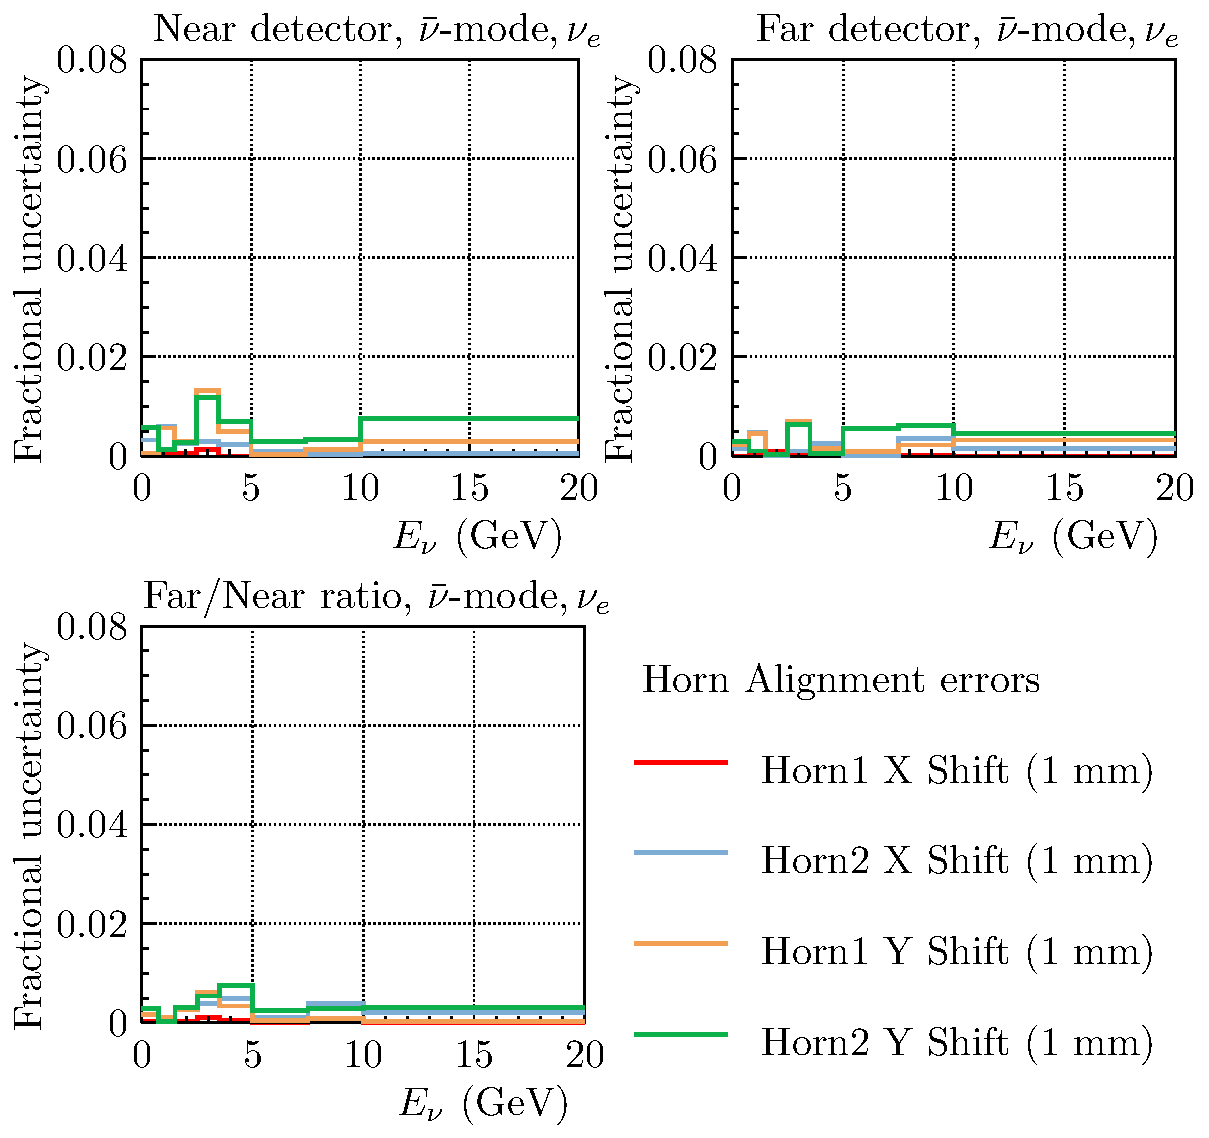
\includegraphics[width=0.65\textwidth]{plots/fracerrs/nubarmode_nue_HornAlignment}
  \caption{The fractional uncertainty due to systematic variations in the alignment of the neutrino horns, the predicted uncertainty on the near prediction, far prediction, and the near/far ratio is shown for electron neutrinos in a antineutrino-mode beam.}
  \label{fig:hornalign_nubar_nue}
\end{figure}

\begin{figure}
  \centering
  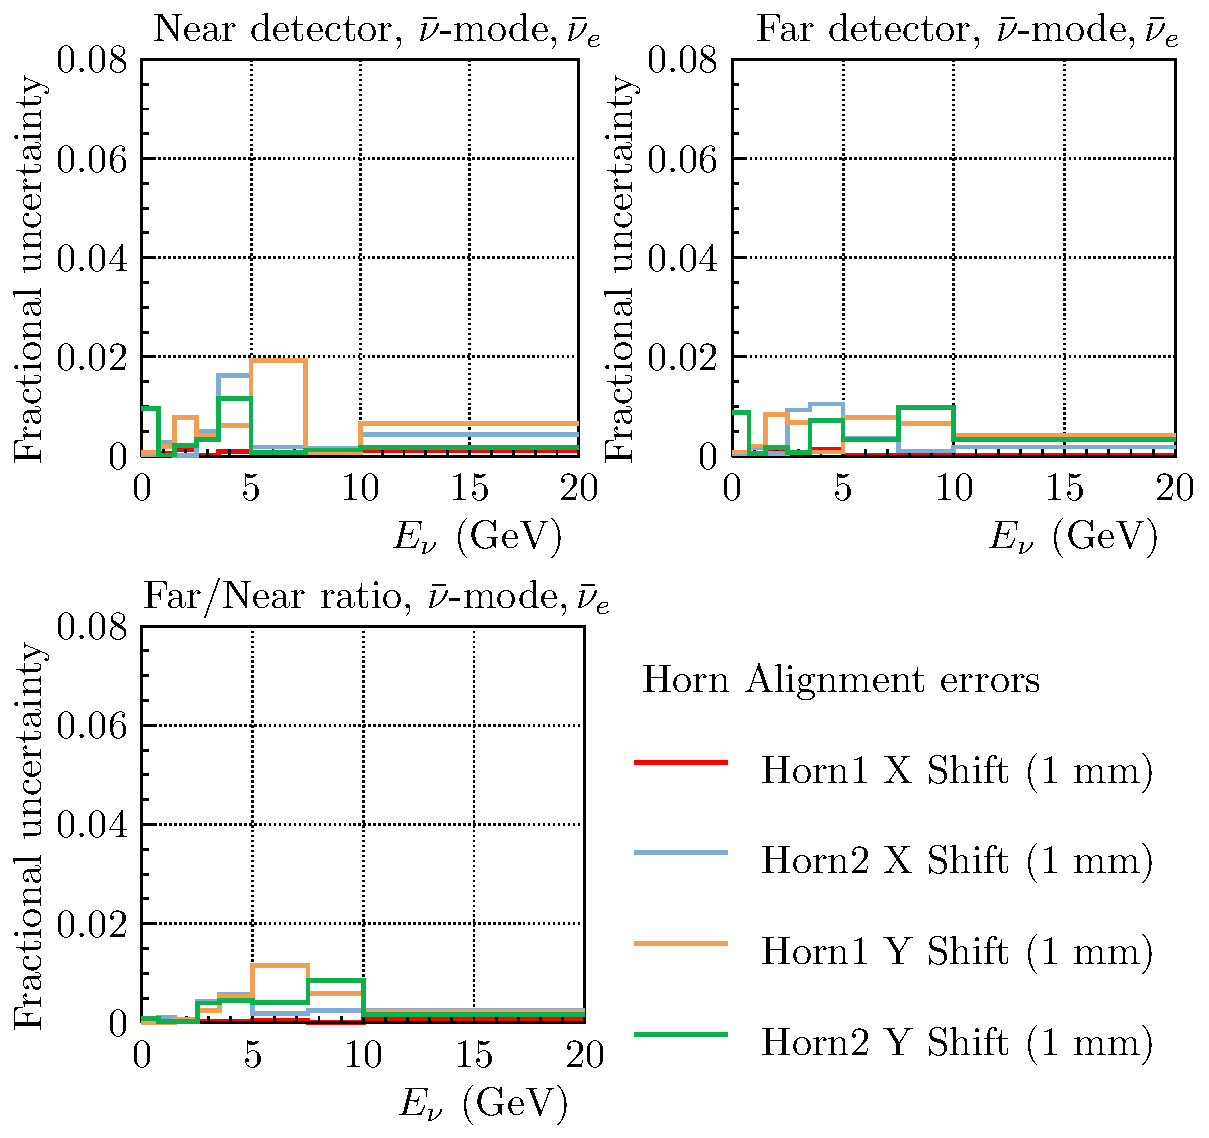
\includegraphics[width=0.65\textwidth]{plots/fracerrs/nubarmode_nuebar_HornAlignment}
  \caption{The fractional uncertainty due to systematic variations in the alignment of the neutrino horns, the predicted uncertainty on the near prediction, far prediction, and the near/far ratio is shown for electron antineutrinos in a antineutrino-mode beam.}
  \label{fig:beamalign_nubar_nuebar}
\end{figure}

\subsection{Beam Alignment}

\begin{figure}
  \centering
  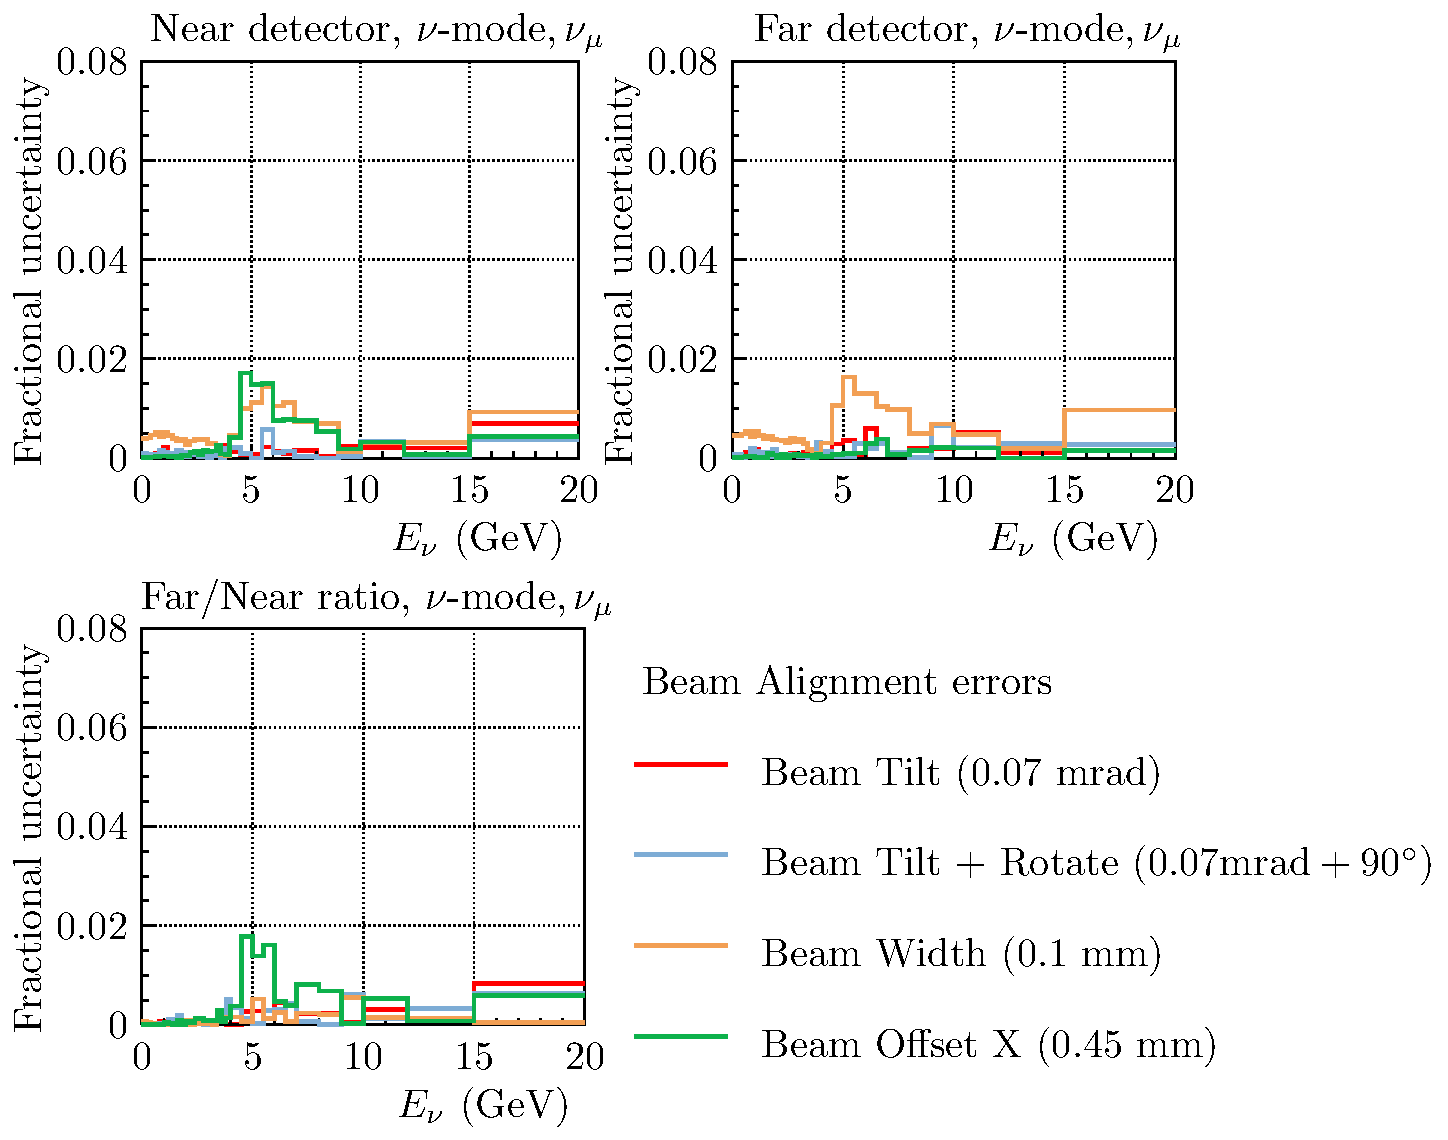
\includegraphics[width=0.65\textwidth]{plots/fracerrs/numode_numu_BeamAlignment}
  \caption{The fractional uncertainty due to systematic variations in alignment of the proton beam onto the target, the predicted uncertainty on the near prediction, far prediction, and the near/far ratio is shown for muon neutrinos in a neutrino-mode beam. }
  \label{fig:beamalign_nu_numu}
\end{figure}

\begin{figure}
  \centering
  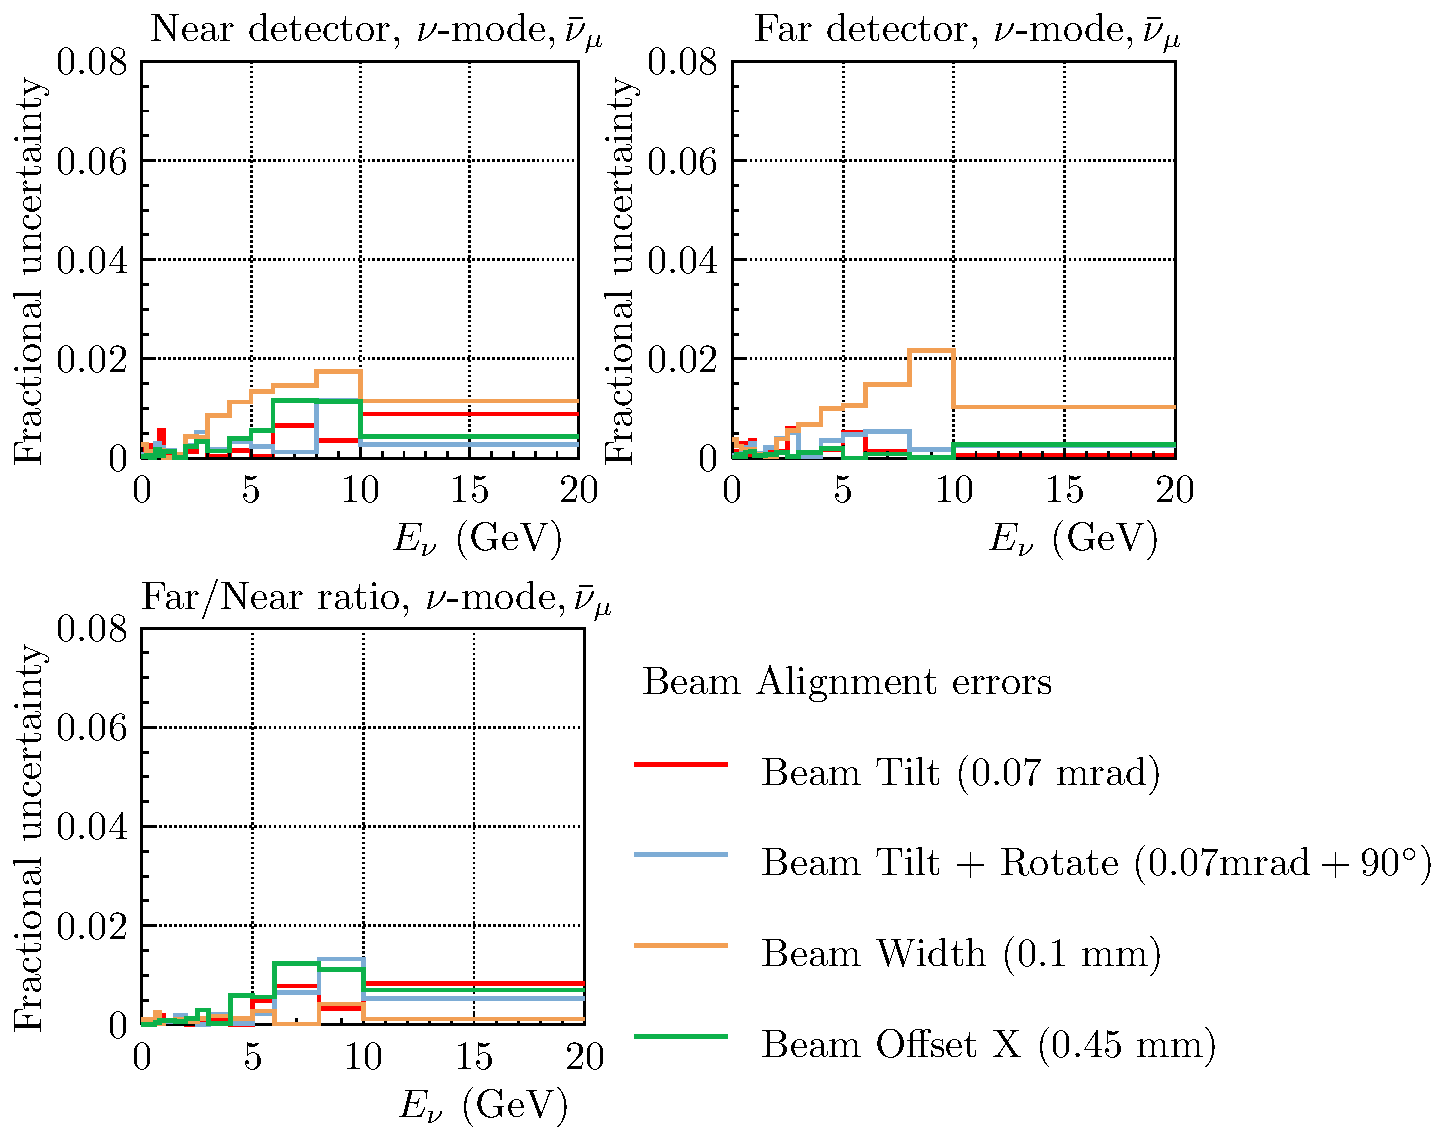
\includegraphics[width=0.65\textwidth]{plots/fracerrs/numode_numubar_BeamAlignment}
  \caption{The fractional uncertainty due to systematic variations in alignment of the proton beam onto the target, the predicted uncertainty on the near prediction, far prediction, and the near/far ratio is shown for muon antineutrinos in a neutrino-mode beam.}
  \label{fig:beamalign_nu_numubar}
\end{figure}

\begin{figure}
  \centering
  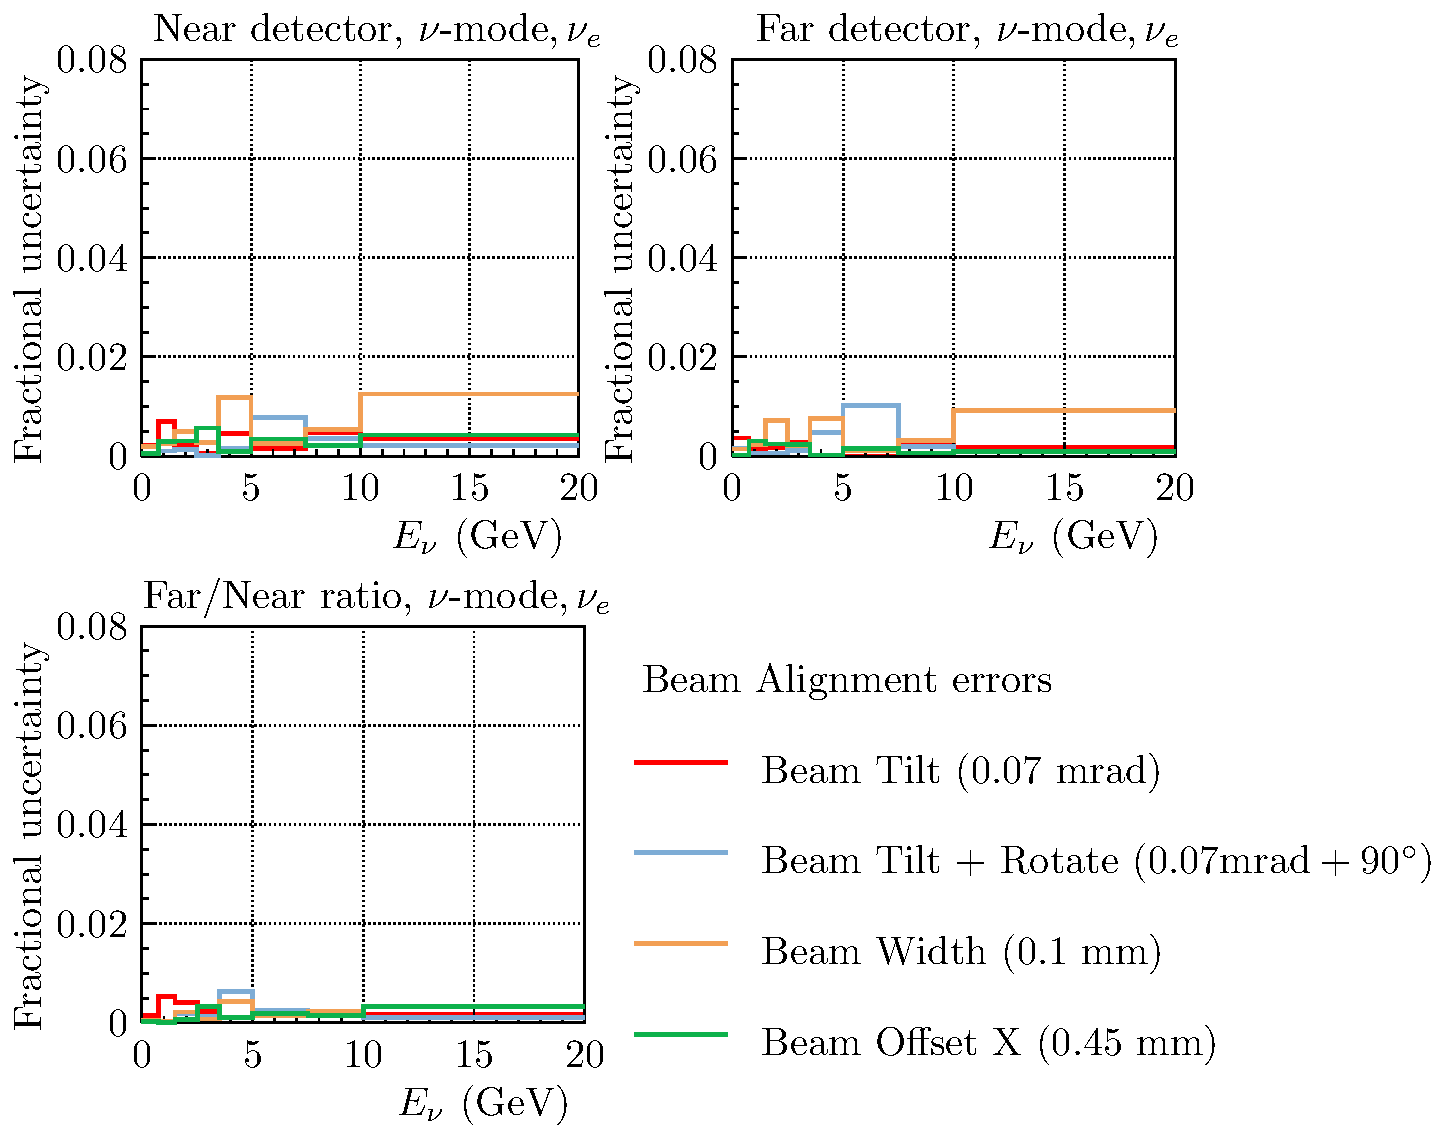
\includegraphics[width=0.65\textwidth]{plots/fracerrs/numode_nue_BeamAlignment}
  \caption{The fractional uncertainty due to systematic variations in alignment of the proton beam onto the target, the predicted uncertainty on the near prediction, far prediction, and the near/far ratio is shown for electron neutrinos in a neutrino-mode beam.}
  \label{fig:beamalign_nu_nue}
\end{figure}

\begin{figure}
  \centering
  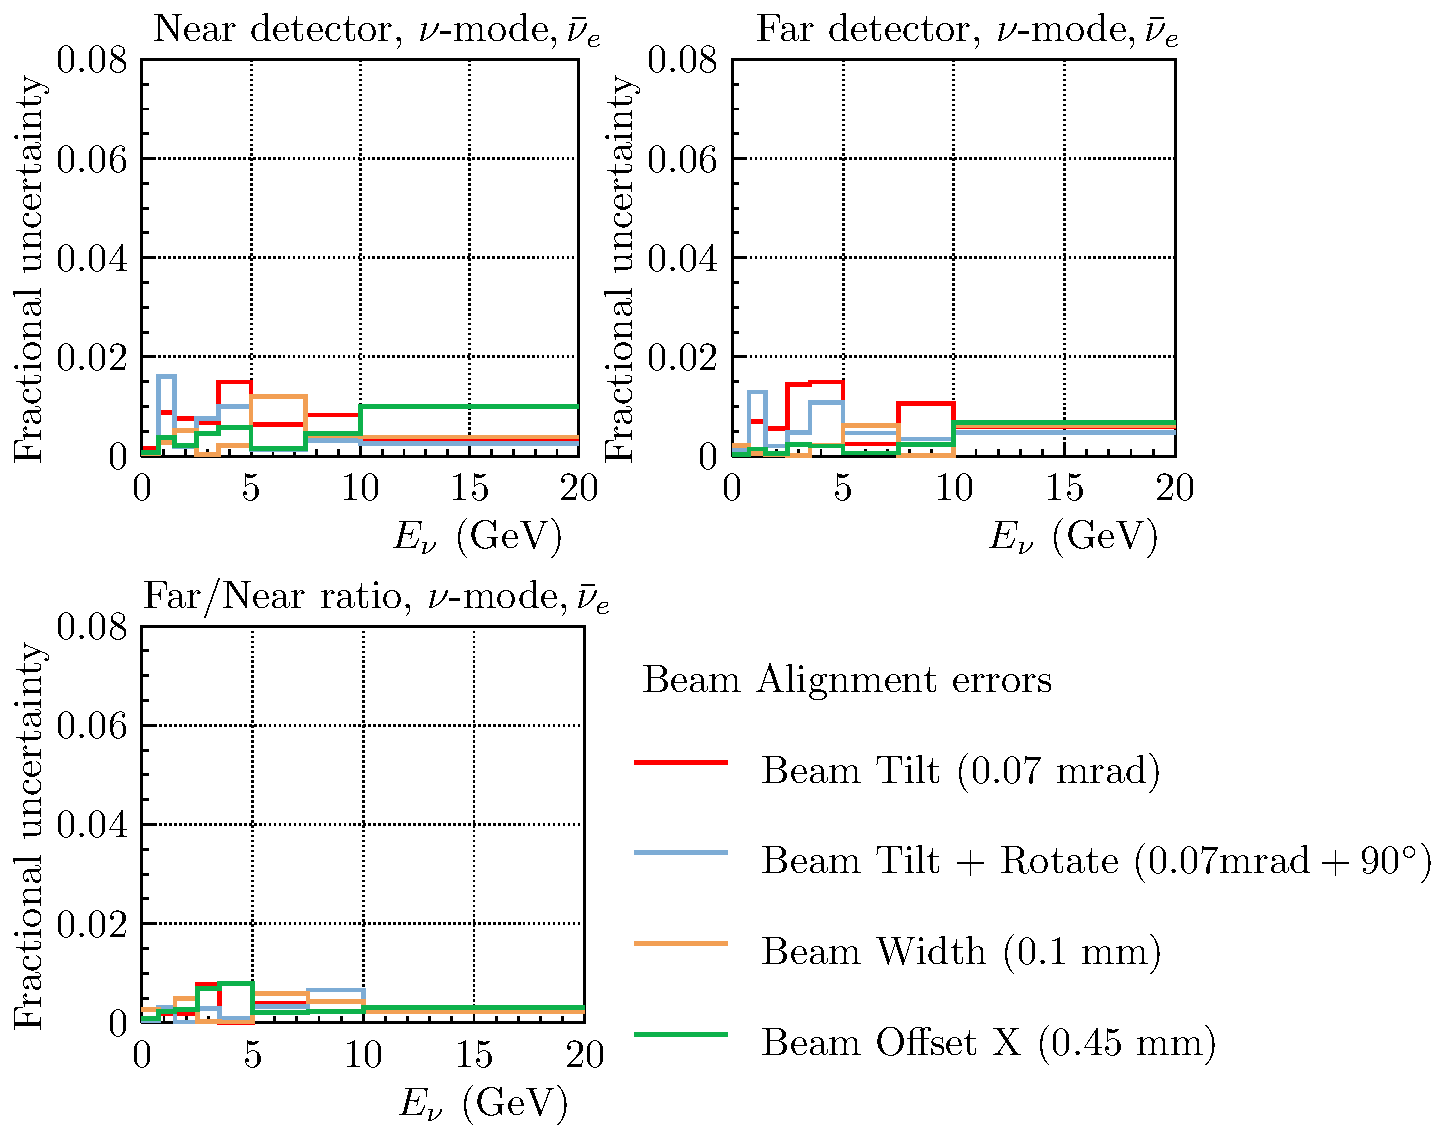
\includegraphics[width=0.65\textwidth]{plots/fracerrs/numode_nuebar_BeamAlignment}
  \caption{The fractional uncertainty due to systematic variations in alignment of the proton beam onto the target, the predicted uncertainty on the near prediction, far prediction, and the near/far ratio is shown for electron antineutrinos in a neutrino-mode beam.}
  \label{fig:beamalign_nu_nuebar}
\end{figure}

\begin{figure}
  \centering
  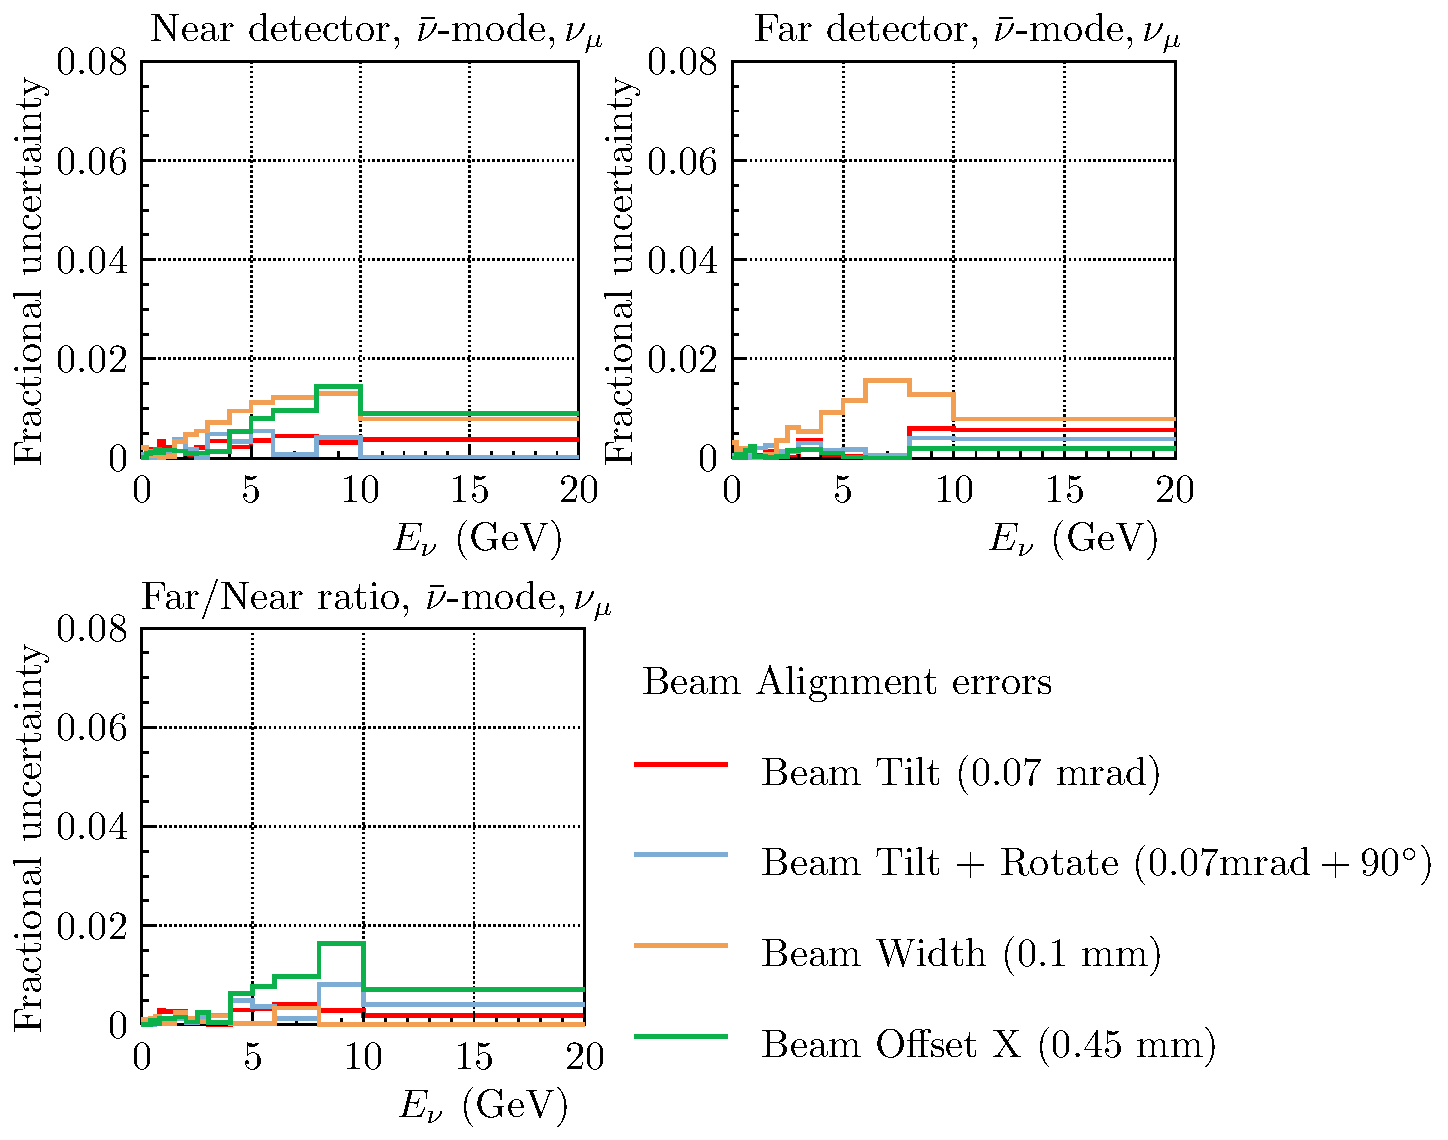
\includegraphics[width=0.65\textwidth]{plots/fracerrs/nubarmode_numu_BeamAlignment}
  \caption{The fractional uncertainty due to systematic variations in alignment of the proton beam onto the target, the predicted uncertainty on the near prediction, far prediction, and the near/far ratio is shown for muon neutrinos in a antineutrino-mode beam.}
  \label{fig:beamalign_nubar_numu}
\end{figure}

\begin{figure}
  \centering
  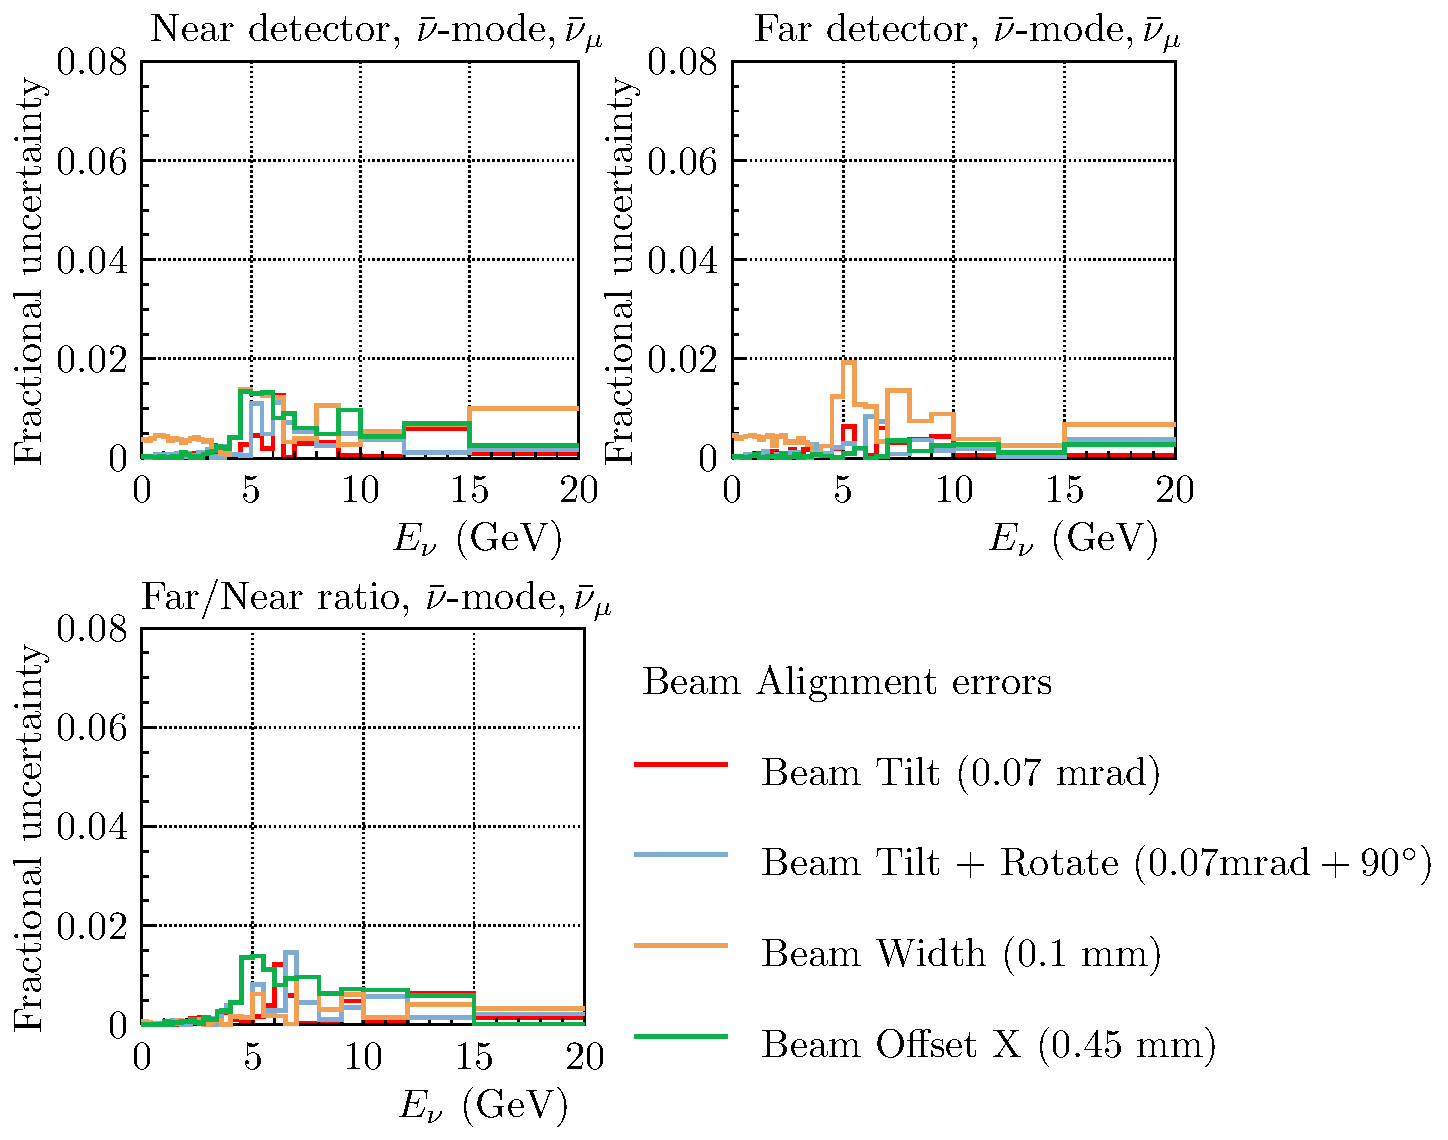
\includegraphics[width=0.65\textwidth]{plots/fracerrs/nubarmode_numubar_BeamAlignment}
  \caption{The fractional uncertainty due to systematic variations in alignment of the proton beam onto the target, the predicted uncertainty on the near prediction, far prediction, and the near/far ratio is shown for muon antineutrinos in a antineutrino-mode beam.}
  \label{fig:beamalign_nubar_numubar}
\end{figure}

\begin{figure}
  \centering
  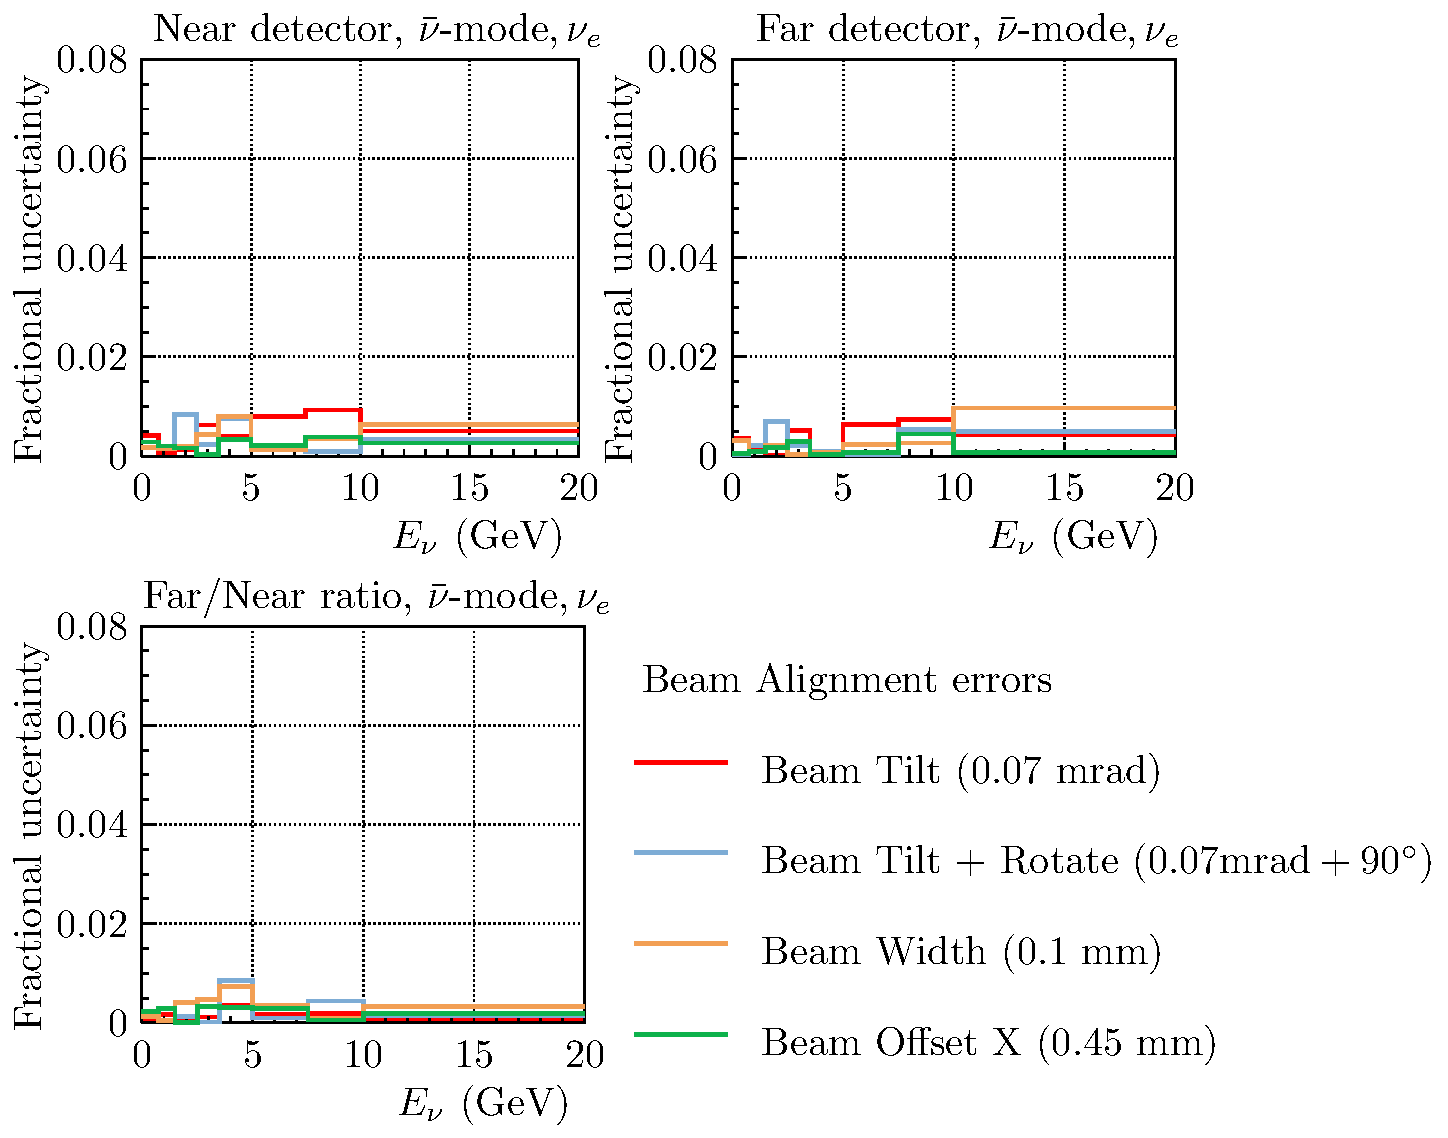
\includegraphics[width=0.65\textwidth]{plots/fracerrs/nubarmode_nue_BeamAlignment}
  \caption{The fractional uncertainty due to systematic variations in alignment of the proton beam onto the target, the predicted uncertainty on the near prediction, far prediction, and the near/far ratio is shown for electron neutrinos in a antineutrino-mode beam.}
  \label{fig:beamalign_nubar_nue}
\end{figure}

\begin{figure}
  \centering
  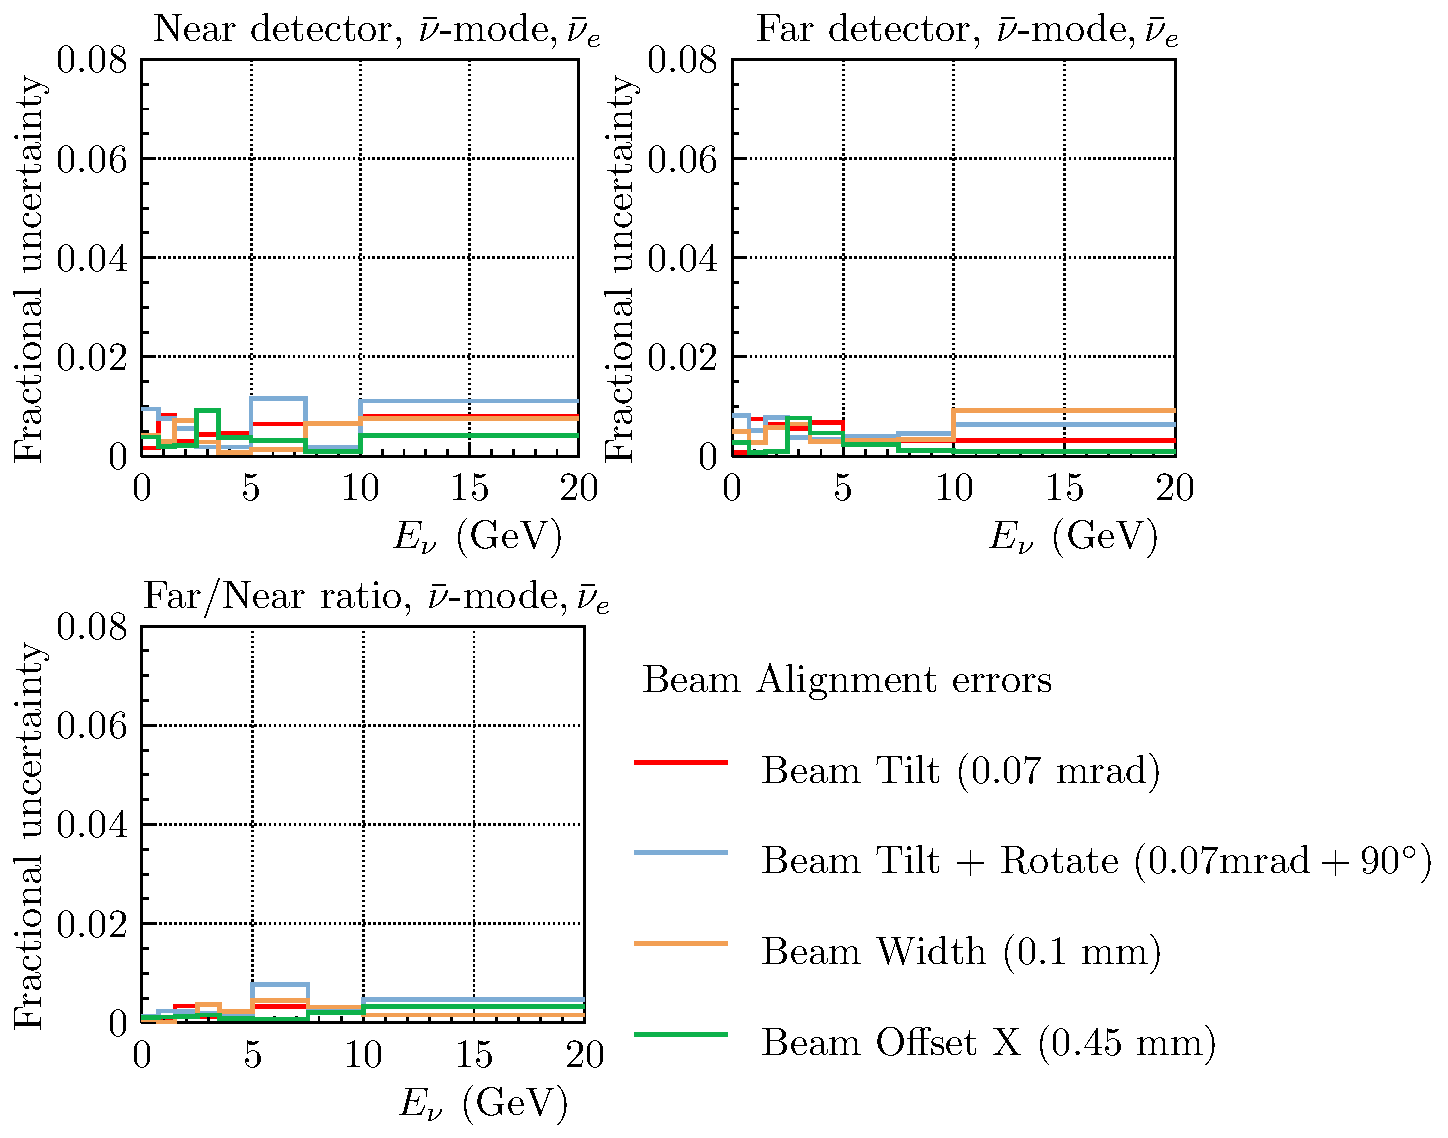
\includegraphics[width=0.65\textwidth]{plots/fracerrs/nubarmode_nuebar_BeamAlignment}
  \caption{The fractional uncertainty due to systematic variations in alignment of the proton beam onto the target, the predicted uncertainty on the near prediction, far prediction, and the near/far ratio is shown for electron antineutrinos in a antineutrino-mode beam.}
  \label{fig:beamalign_nubar_nuebar}
\end{figure}

\subsection{Grouped}

\begin{figure}
  \centering
  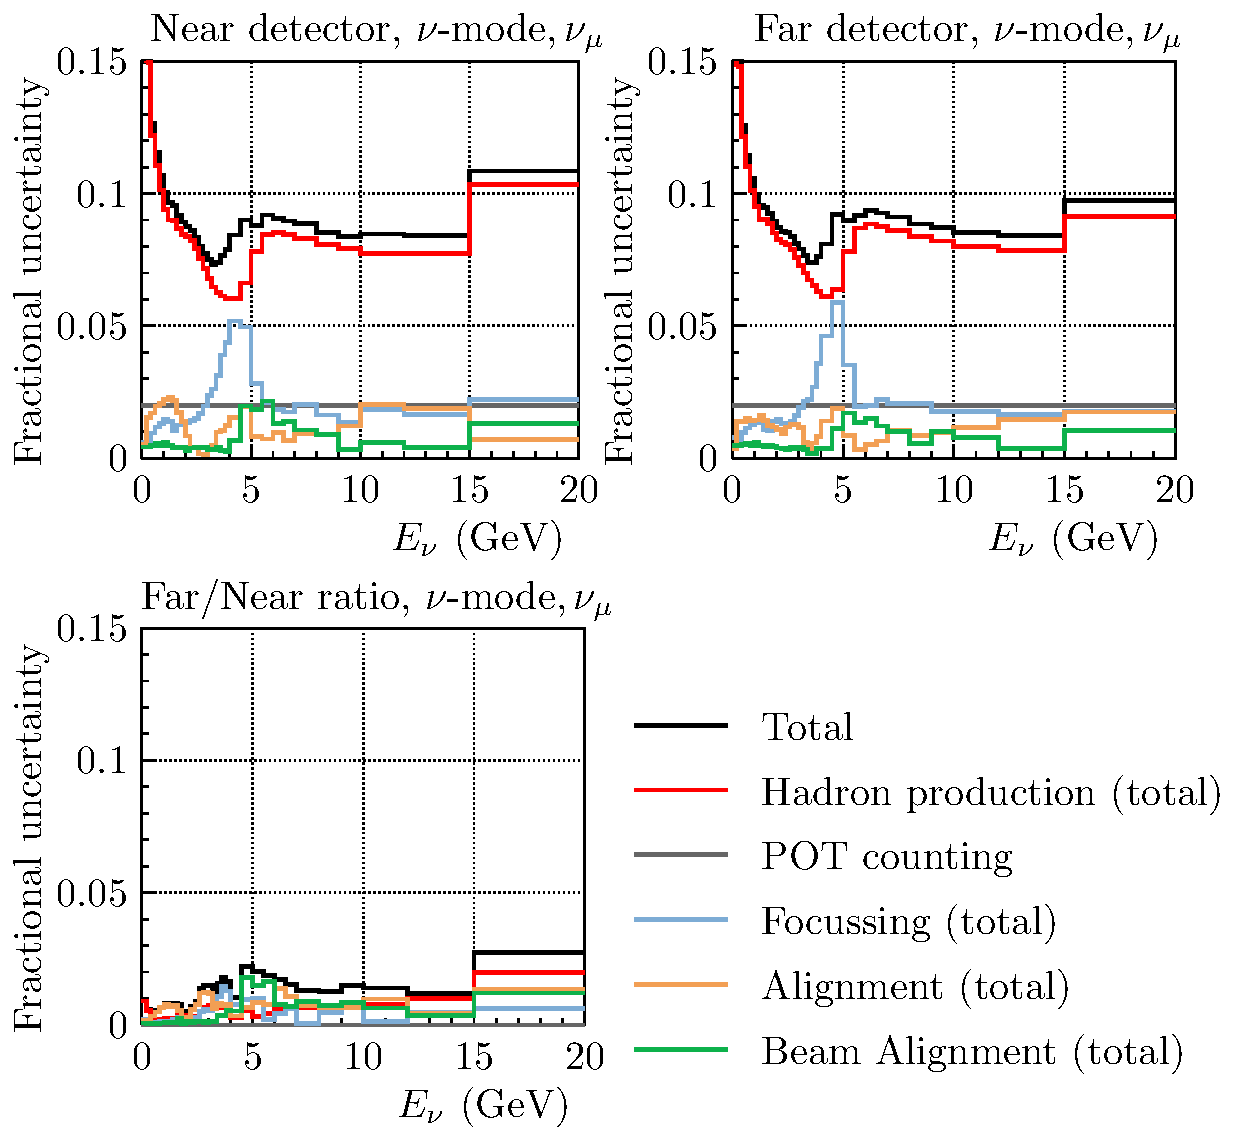
\includegraphics[width=0.65\textwidth]{plots/fracerrs/numode_numu_ErrType}
  \caption{The fractional uncertainty due to groups of systematic variations in the neutrino beam simulation, the predicted uncertainty on the near prediction, far prediction, and the near/far ratio is shown for muon neutrinos in a neutrino-mode beam. }
  \label{fig:grp_nu_numu}
\end{figure}

\begin{figure}
  \centering
  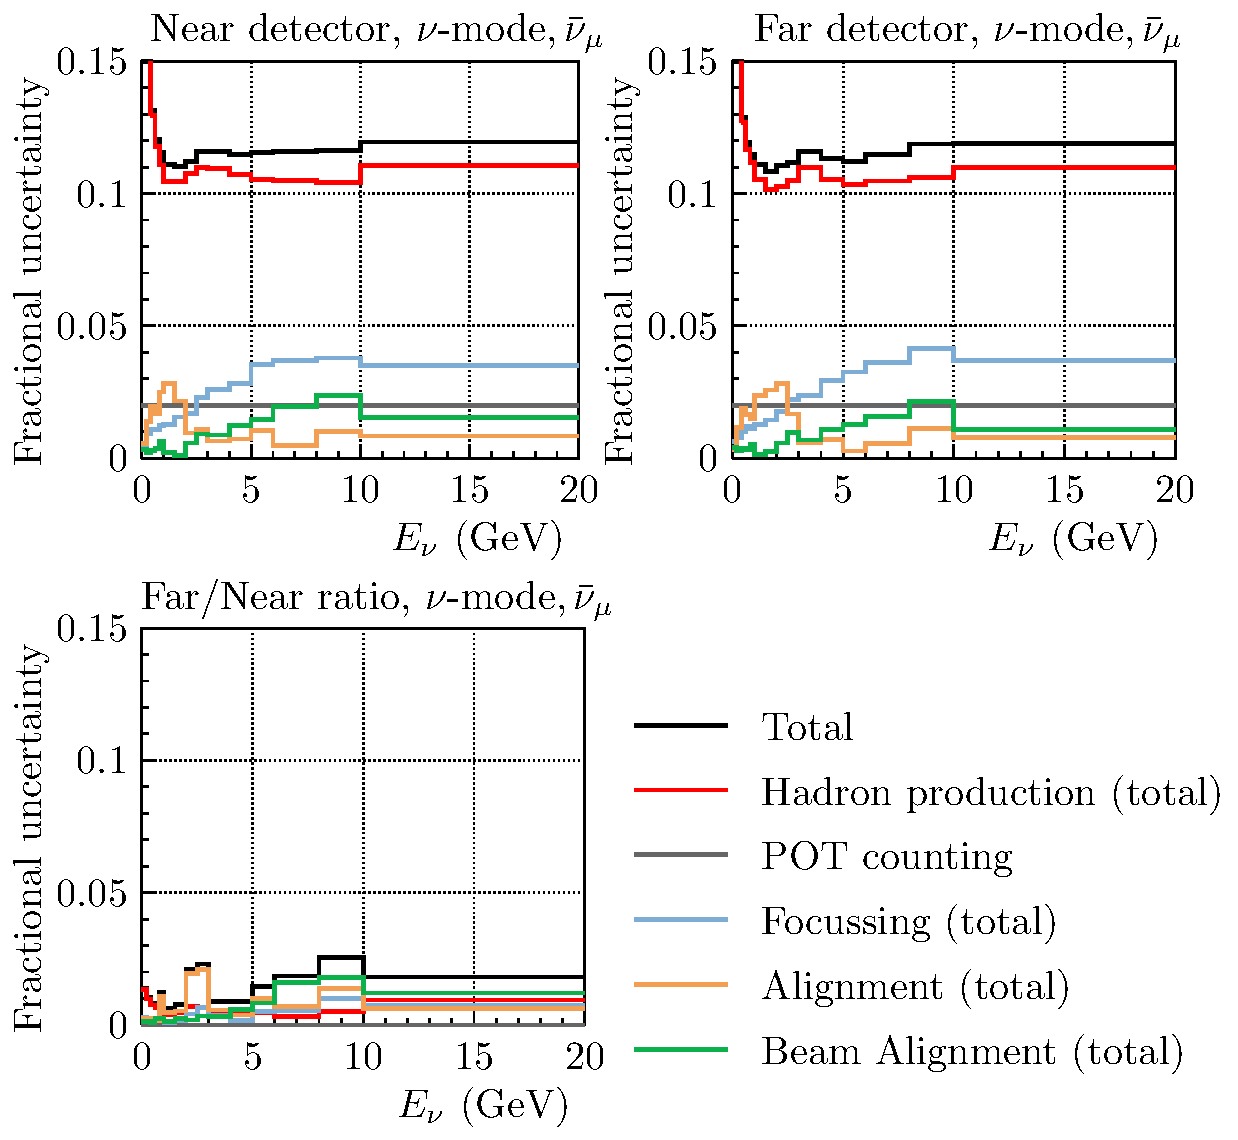
\includegraphics[width=0.65\textwidth]{plots/fracerrs/numode_numubar_ErrType}
  \caption{The fractional uncertainty due to groups of systematic variations in the neutrino beam simulation, the predicted uncertainty on the near prediction, far prediction, and the near/far ratio is shown for muon antineutrinos in a neutrino-mode beam.}
  \label{fig:grp_nu_numubar}
\end{figure}

\begin{figure}
  \centering
  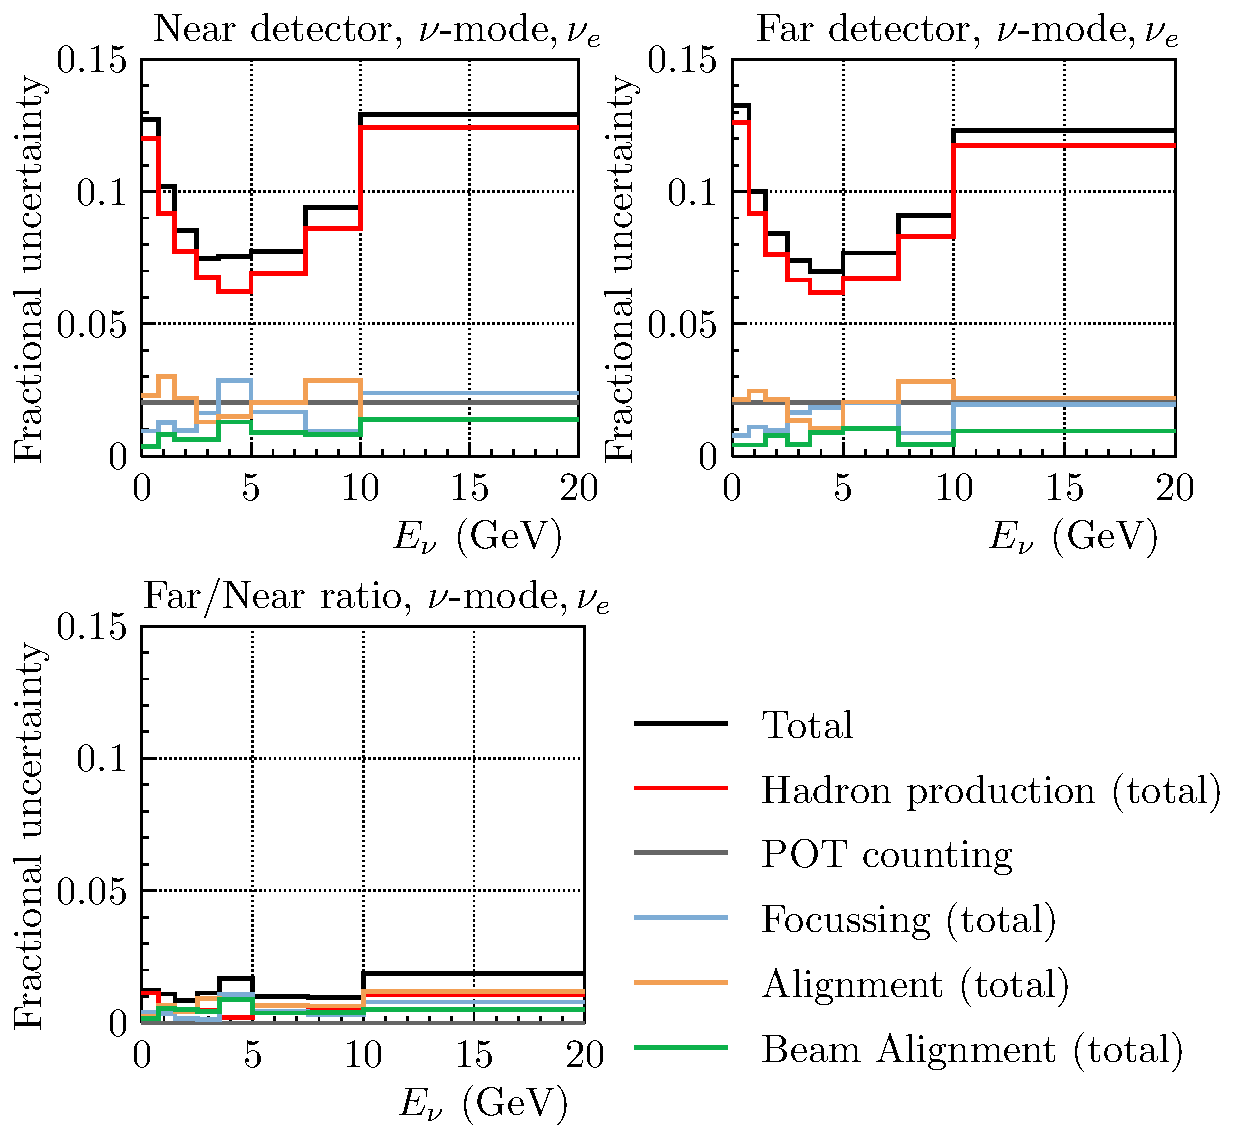
\includegraphics[width=0.65\textwidth]{plots/fracerrs/numode_nue_ErrType}
  \caption{The fractional uncertainty due to groups of systematic variations in the neutrino beam simulation, the predicted uncertainty on the near prediction, far prediction, and the near/far ratio is shown for electron neutrinos in a neutrino-mode beam.}
  \label{fig:grp_nu_nue}
\end{figure}

\begin{figure}
  \centering
  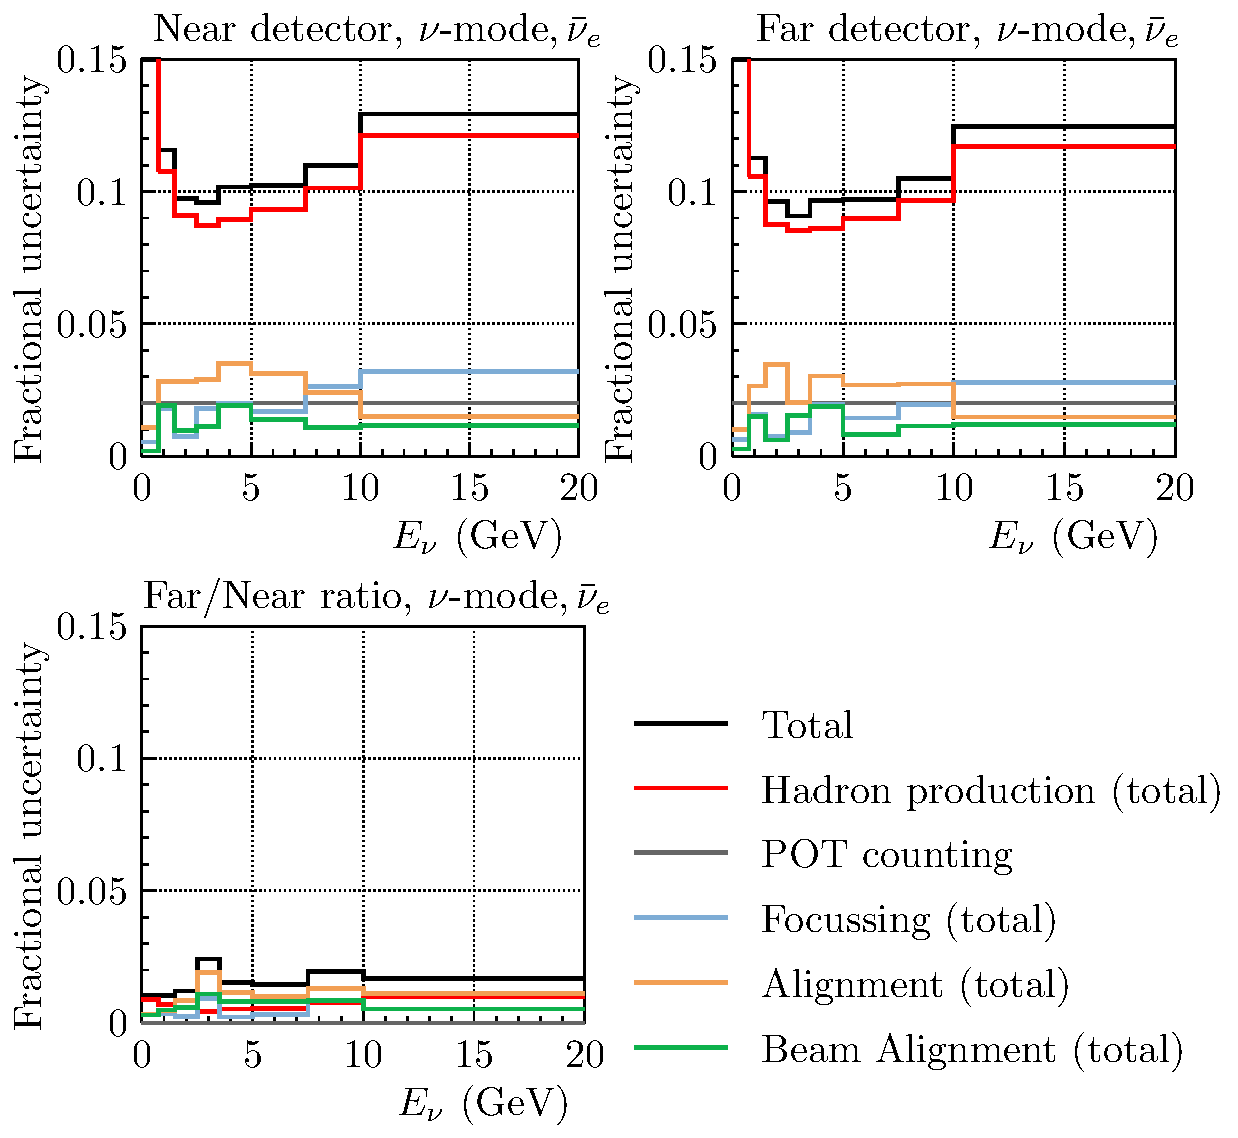
\includegraphics[width=0.65\textwidth]{plots/fracerrs/numode_nuebar_ErrType}
  \caption{The fractional uncertainty due to groups of systematic variations in the neutrino beam simulation, the predicted uncertainty on the near prediction, far prediction, and the near/far ratio is shown for electron antineutrinos in a neutrino-mode beam.}
  \label{fig:grp_nu_nuebar}
\end{figure}

\begin{figure}
  \centering
  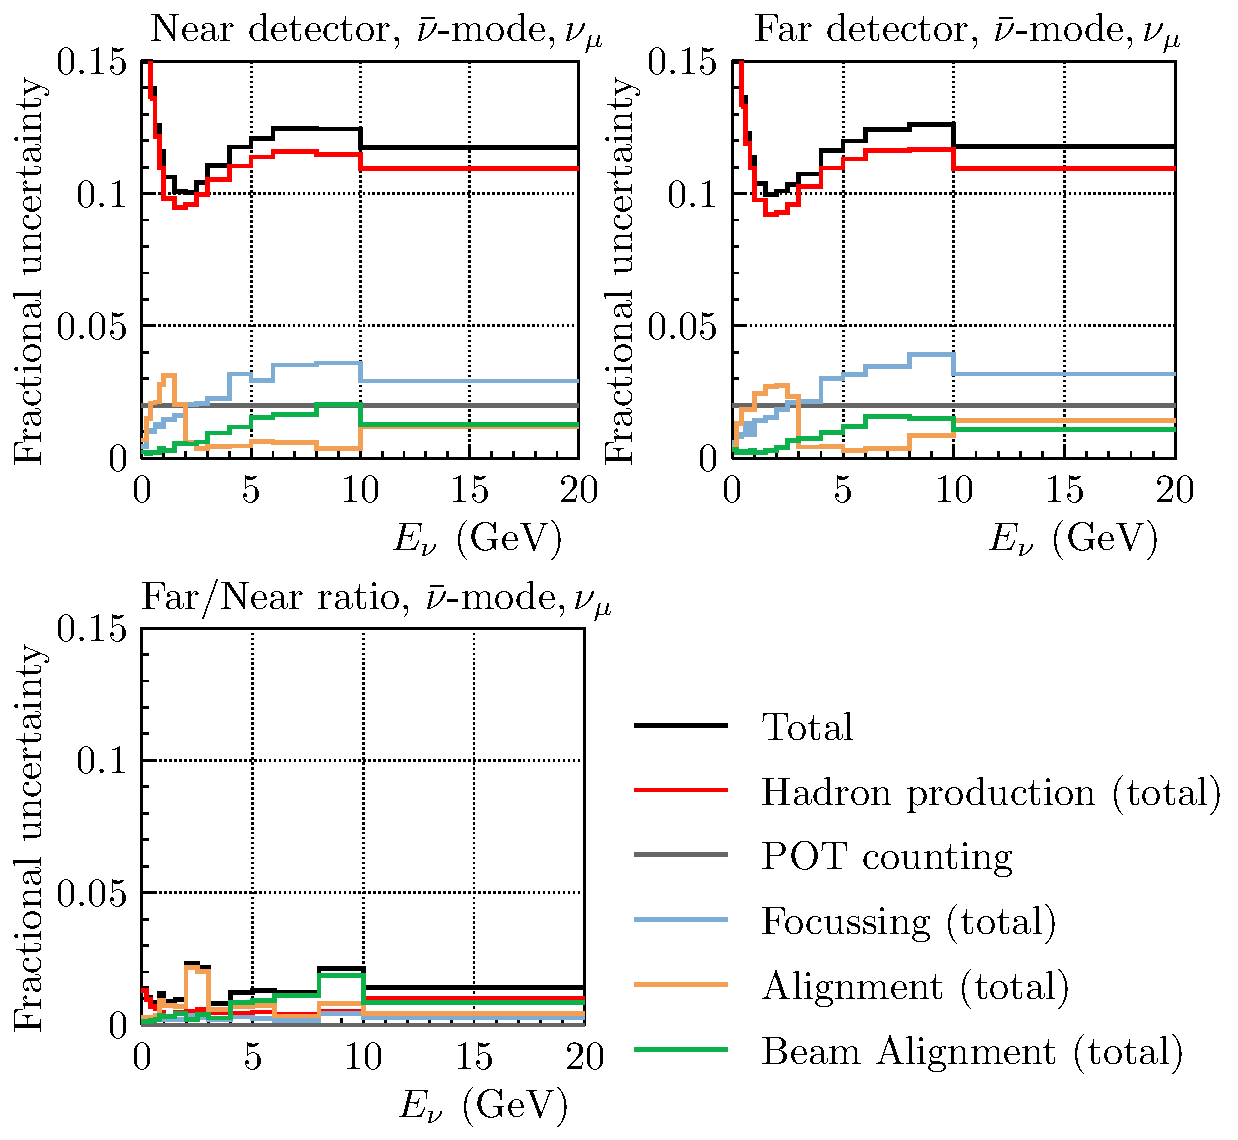
\includegraphics[width=0.65\textwidth]{plots/fracerrs/nubarmode_numu_ErrType}
  \caption{The fractional uncertainty due to groups of systematic variations in the neutrino beam simulation, the predicted uncertainty on the near prediction, far prediction, and the near/far ratio is shown for muon neutrinos in a antineutrino-mode beam.}
  \label{fig:grp_nubar_numu}
\end{figure}

\begin{figure}
  \centering
  \includegraphics[width=0.65\textwidth]{plots/fracerrs/nubarmode_numubar_ErrType}
  \caption{The fractional uncertainty due to groups of systematic variations in the neutrino beam simulation, the predicted uncertainty on the near prediction, far prediction, and the near/far ratio is shown for muon antineutrinos in a antineutrino-mode beam.}
  \label{fig:grp_nubar_numubar}
\end{figure}

\begin{figure}
  \centering
  \includegraphics[width=0.65\textwidth]{plots/fracerrs/nubarmode_nue_ErrType}
  \caption{The fractional uncertainty due to groups of systematic variations in the neutrino beam simulation, the predicted uncertainty on the near prediction, far prediction, and the near/far ratio is shown for electron neutrinos in a antineutrino-mode beam.}
  \label{fig:grp_nubar_nue}
\end{figure}

\begin{figure}
  \centering
  \includegraphics[width=0.65\textwidth]{plots/fracerrs/nubarmode_nuebar_ErrType}
  \caption{The fractional uncertainty due to groups of systematic variations in the neutrino beam simulation, the predicted uncertainty on the near prediction, far prediction, and the near/far ratio is shown for electron antineutrinos in a antineutrino-mode beam.}
  \label{fig:grp_nubar_nuebar}
\end{figure}

\subsection{Grouped off axis}

\begin{figure}
  \centering
  \includegraphics[width=\textwidth]{plots/fracerrs/numode_numu_ErrType_OffAxis}
  \caption{The fractional uncertainty due to groups of systematic variations in the neutrino beam simulation, the predicted uncertainty on the near prediction at 6 on and off axis positions is compared }
  \label{fig:grp_nu_numu_offaxis}
\end{figure}

\begin{figure}
  \centering
  \includegraphics[width=\textwidth]{plots/fracerrs/numode_numubar_ErrType_OffAxis}
  \caption{The fractional uncertainty due to groups of systematic variations in the neutrino beam simulation, the predicted uncertainty on the near prediction at 6 on and off axis positions is compared.}
  \label{fig:grp_nu_numubar_offaxis}
\end{figure}

\begin{figure}
  \centering
  \includegraphics[width=\textwidth]{plots/fracerrs/numode_nue_ErrType_OffAxis}
  \caption{The fractional uncertainty due to groups of systematic variations in the neutrino beam simulation, the predicted uncertainty on the near prediction at 6 on and off axis positions is compared.}
  \label{fig:grp_nu_nue_offaxis}
\end{figure}

\begin{figure}
  \centering
  \includegraphics[width=\textwidth]{plots/fracerrs/numode_nuebar_ErrType_OffAxis}
  \caption{The fractional uncertainty due to groups of systematic variations in the neutrino beam simulation, the predicted uncertainty on the near prediction at 6 on and off axis positions is compared.}
  \label{fig:grp_nu_nuebar_offaxis}
\end{figure}

\begin{figure}
  \centering
  \includegraphics[width=\textwidth]{plots/fracerrs/nubarmode_numu_ErrType_OffAxis}
  \caption{The fractional uncertainty due to groups of systematic variations in the neutrino beam simulation, the predicted uncertainty on the near prediction at 6 on and off axis positions is compared.}
  \label{fig:grp_nubar_numu_offaxis}
\end{figure}

\begin{figure}
  \centering
  \includegraphics[width=\textwidth]{plots/fracerrs/nubarmode_numubar_ErrType_OffAxis}
  \caption{The fractional uncertainty due to groups of systematic variations in the neutrino beam simulation, the predicted uncertainty on the near prediction at 6 on and off axis positions is compared.}
  \label{fig:grp_nubar_numubar_offaxis}
\end{figure}

\begin{figure}
  \centering
  \includegraphics[width=\textwidth]{plots/fracerrs/nubarmode_nue_ErrType_OffAxis}
  \caption{The fractional uncertainty due to groups of systematic variations in the neutrino beam simulation, the predicted uncertainty on the near prediction at 6 on and off axis positions is compared.}
  \label{fig:grp_nubar_nue_offaxis}
\end{figure}

\begin{figure}
  \centering
  \includegraphics[width=\textwidth]{plots/fracerrs/nubarmode_nuebar_ErrType_OffAxis}
  \caption{The fractional uncertainty due to groups of systematic variations in the neutrino beam simulation, the predicted uncertainty on the near prediction at 6 on and off axis positions is compared.}
  \label{fig:grp_nubar_nuebar_offaxis}
\end{figure}

\section{Terms}

\begin{itemize}
\item $\nu$-mode, positive horn current, and mostly matter beam are used interchangeably, with the first being the preferred form.
\item $\bar{\nu}$-mode, negative horn current, mostly anti-matter beam are used interchangeably, with the first being the preferred form.
\end{itemize}


\end{document}
